\chapter{TCK Acceptance Tests}

\section{OptionalMatch}

\subsection{Satisfies the open world assumption, relationships between same nodes}

\begin{lstlisting}
MATCH (p:Player)-[:PLAYS_FOR]->(team:Team)
OPTIONAL MATCH (p)-[s:SUPPORTS]->(team)
RETURN count(*) AS matches, s IS NULL AS optMatch
\end{lstlisting}

Cannot visualize
\subsection{Satisfies the open world assumption, single relationship}

\begin{lstlisting}
MATCH (p:Player)-[:PLAYS_FOR]->(team:Team)
OPTIONAL MATCH (p)-[s:SUPPORTS]->(team)
RETURN count(*) AS matches, s IS NULL AS optMatch
\end{lstlisting}

Cannot visualize
\subsection{Satisfies the open world assumption, relationships between different nodes}

\begin{lstlisting}
MATCH (p:Player)-[:PLAYS_FOR]->(team:Team)
OPTIONAL MATCH (p)-[s:SUPPORTS]->(team)
RETURN count(*) AS matches, s IS NULL AS optMatch
\end{lstlisting}

Cannot visualize
\section{MatchAcceptance2}

\subsection{Do not return non-existent nodes}

\begin{lstlisting}
MATCH (n)
RETURN n
\end{lstlisting}

\begin{tikzpicture}
\linespread{1.25}
\Tree
[. {$\projection{\var{n}}$ \\ \footnotesize $\color{gray} \langle \var{n} \rangle$}
	[. {$\getvertices{n}{}$ \\ \footnotesize $\color{gray} \langle \var{n} \rangle$}
	]
]
;
\end{tikzpicture}
\subsection{Do not return non-existent relationships}

\begin{lstlisting}
MATCH ()-[r]->()
RETURN r
\end{lstlisting}

\begin{tikzpicture}
\linespread{1.25}
\Tree
[. {$\projection{\var{r}}$ \\ \footnotesize $\color{gray} \langle \var{r} \rangle$}
	[. {$\expandout{r}{}{\_e1}{\_e2}{}$ \\ \footnotesize $\color{gray} \langle \var{\_e1, r, \_e2} \rangle$}
		[. {$\getvertices{\_e1}{}$ \\ \footnotesize $\color{gray} \langle \var{\_e1} \rangle$}
		]
	]
]
;
\end{tikzpicture}
\subsection{Do not fail when evaluating predicates with illegal operations if the AND'ed predicate evaluates to false}

\begin{lstlisting}
MATCH (:Root {name: 'x'})-->(i:TextNode)
WHERE i.id > 'te'
RETURN i
\end{lstlisting}

Cannot visualize
\subsection{Do not fail when evaluating predicates with illegal operations if the OR'd predicate evaluates to true}

\begin{lstlisting}
MATCH (:Root {name: 'x'})-->(i)
WHERE exists(i.id) OR i.id > 'te'
RETURN i
\end{lstlisting}

Cannot visualize
\subsection{Aggregation with named paths}

\begin{lstlisting}
MATCH p = ()-[*]->()
WITH count(*) AS count, p AS p
WITH nodes(p) AS nodes
RETURN *
\end{lstlisting}

Cannot visualize
\subsection{Zero-length variable length pattern in the middle of the pattern}

\begin{lstlisting}
MATCH (a {name: 'A'})-[:CONTAINS*0..1]->(b)-[:FRIEND*0..1]->(c)
RETURN a, b, c
\end{lstlisting}

Cannot visualize
\subsection{Simple variable length pattern}

\begin{lstlisting}
MATCH (a {name: 'A'})-[*]->(x)
RETURN x
\end{lstlisting}

Cannot visualize
\subsection{Variable length relationship without lower bound}

\begin{lstlisting}
MATCH p = ({name: 'A'})-[:KNOWS*..2]->()
RETURN p
\end{lstlisting}

Cannot visualize
\subsection{Variable length relationship without bounds}

\begin{lstlisting}
MATCH p = ({name: 'A'})-[:KNOWS*..]->()
RETURN p
\end{lstlisting}

Cannot visualize
\subsection{Returning bound nodes that are not part of the pattern}

\begin{lstlisting}
MATCH (a {name: 'A'}), (c {name: 'C'})
MATCH (a)-->(b)
RETURN a, b, c
\end{lstlisting}

Cannot visualize
\subsection{Two bound nodes pointing to the same node}

\begin{lstlisting}
MATCH (a {name: 'A'}), (b {name: 'B'})
MATCH (a)-->(x)<-->(b)
RETURN x
\end{lstlisting}

Cannot visualize
\subsection{Three bound nodes pointing to the same node}

\begin{lstlisting}
MATCH (a {name: 'A'}), (b {name: 'B'}), (c {name: 'C'})
MATCH (a)-->(x), (b)-->(x), (c)-->(x)
RETURN x
\end{lstlisting}

Cannot visualize
\subsection{Three bound nodes pointing to the same node with extra connections}

\begin{lstlisting}
MATCH (a {name: 'a'}), (b {name: 'b'}), (c {name: 'c'})
MATCH (a)-->(x), (b)-->(x), (c)-->(x)
RETURN x
\end{lstlisting}

Cannot visualize
\subsection{MATCH with OPTIONAL MATCH in longer pattern}

\begin{lstlisting}
MATCH (a {name: 'A'})
OPTIONAL MATCH (a)-[:KNOWS]->()-[:KNOWS]->(foo)
RETURN foo
\end{lstlisting}

Cannot visualize
\subsection{Optionally matching named paths}

\begin{lstlisting}
MATCH (a {name: 'A'}), (x)
WHERE x.name IN ['B', 'C']
OPTIONAL MATCH p = (a)-->(x)
RETURN x, p
\end{lstlisting}

Cannot visualize
\subsection{Optionally matching named paths with single and variable length patterns}

\begin{lstlisting}
MATCH (a {name: 'A'})
OPTIONAL MATCH p = (a)-->(b)-[*]->(c)
RETURN p
\end{lstlisting}

Cannot visualize
\subsection{Optionally matching named paths with variable length patterns}

\begin{lstlisting}
MATCH (a {name: 'A'}), (x)
WHERE x.name IN ['B', 'C']
OPTIONAL MATCH p = (a)-[r*]->(x)
RETURN r, x, p
\end{lstlisting}

Cannot visualize
\subsection{Matching variable length patterns from a bound node}

\begin{lstlisting}
MATCH (a:A)
MATCH (a)-[r*2]->()
RETURN r
\end{lstlisting}

Cannot visualize
\subsection{Excluding connected nodes}

\begin{lstlisting}
MATCH (a:A), (other:B)
OPTIONAL MATCH (a)-[r]->(other)
WITH other WHERE r IS NULL
RETURN other
\end{lstlisting}

Cannot visualize
\subsection{Do not fail when predicates on optionally matched and missed nodes are invalid}

\begin{lstlisting}
MATCH (n)-->(x0)
OPTIONAL MATCH (x0)-->(x1)
WHERE x1.foo = 'bar'
RETURN x0.name
\end{lstlisting}

\begin{tikzpicture}
\linespread{1.25}
\Tree
[. {$\projection{\var{x0}}$ \\ \footnotesize $\color{gray} \langle \var{x0} \rangle$}
	[. {$\join \{\var{x0}\}$ \\ \footnotesize $\color{gray} \langle \var{n, \_e1, x0, \_e2, x1} \rangle$}
		[. {$\expandout{\_e1}{}{n}{x0}{}$ \\ \footnotesize $\color{gray} \langle \var{n, \_e1, x0} \rangle$}
			[. {$\getvertices{n}{}$ \\ \footnotesize $\color{gray} \langle \var{n} \rangle$}
			]
		]
		[. {$\selection{\mathtt{x1.foo~=~'bar'}}$ \\ \footnotesize $\color{gray} \langle \var{x0, \_e2, x1} \rangle$}
			[. {$\expandout{\_e2}{}{x0}{x1}{}$ \\ \footnotesize $\color{gray} \langle \var{x0, \_e2, x1} \rangle$}
				[. {$\getvertices{x0}{}$ \\ \footnotesize $\color{gray} \langle \var{x0} \rangle$}
				]
			]
		]
	]
]
;
\end{tikzpicture}
\subsection{MATCH and OPTIONAL MATCH on same pattern}

\begin{lstlisting}
MATCH (a)-->(b)
WHERE b:B
OPTIONAL MATCH (a)-->(c)
WHERE c:C
RETURN a.name
\end{lstlisting}

\begin{tikzpicture}
\linespread{1.25}
\Tree
[. {$\projection{\var{a}}$ \\ \footnotesize $\color{gray} \langle \var{a} \rangle$}
	[. {$\join \{\var{a}\}$ \\ \footnotesize $\color{gray} \langle \var{a, \_e1, b, \_e2, c} \rangle$}
		[. {$\selection{\mathtt{b:B}}$ \\ \footnotesize $\color{gray} \langle \var{a, \_e1, b} \rangle$}
			[. {$\expandout{\_e1}{}{a}{b}{}$ \\ \footnotesize $\color{gray} \langle \var{a, \_e1, b} \rangle$}
				[. {$\getvertices{a}{}$ \\ \footnotesize $\color{gray} \langle \var{a} \rangle$}
				]
			]
		]
		[. {$\selection{\mathtt{c:C}}$ \\ \footnotesize $\color{gray} \langle \var{a, \_e2, c} \rangle$}
			[. {$\expandout{\_e2}{}{a}{c}{}$ \\ \footnotesize $\color{gray} \langle \var{a, \_e2, c} \rangle$}
				[. {$\getvertices{a}{}$ \\ \footnotesize $\color{gray} \langle \var{a} \rangle$}
				]
			]
		]
	]
]
;
\end{tikzpicture}
\subsection{Matching using an undirected pattern}

\begin{lstlisting}
MATCH (a)-[:ADMIN]-(b)
WHERE a:A
RETURN a.id, b.id
\end{lstlisting}

\begin{tikzpicture}
\linespread{1.25}
\Tree
[. {$\projection{\var{a},~\var{b}}$ \\ \footnotesize $\color{gray} \langle \var{a, b} \rangle$}
	[. {$\selection{\mathtt{a:A}}$ \\ \footnotesize $\color{gray} \langle \var{a, \_e1, b} \rangle$}
		[. {$\expandboth{\_e1}{ADMIN}{a}{b}{}$ \\ \footnotesize $\color{gray} \langle \var{a, \_e1, b} \rangle$}
			[. {$\getvertices{a}{}$ \\ \footnotesize $\color{gray} \langle \var{a} \rangle$}
			]
		]
	]
]
;
\end{tikzpicture}
\subsection{Matching all nodes}

\begin{lstlisting}
MATCH (n)
RETURN n
\end{lstlisting}

\begin{tikzpicture}
\linespread{1.25}
\Tree
[. {$\projection{\var{n}}$ \\ \footnotesize $\color{gray} \langle \var{n} \rangle$}
	[. {$\getvertices{n}{}$ \\ \footnotesize $\color{gray} \langle \var{n} \rangle$}
	]
]
;
\end{tikzpicture}
\subsection{Comparing nodes for equality}

\begin{lstlisting}
MATCH (a), (b)
WHERE a <> b
RETURN a, b
\end{lstlisting}

\begin{tikzpicture}
\linespread{1.25}
\Tree
[. {$\projection{\var{a},~\var{b}}$ \\ \footnotesize $\color{gray} \langle \var{a, b} \rangle$}
	[. {$\selection{\mathtt{a~<>~b}}$ \\ \footnotesize $\color{gray} \langle \var{a, b} \rangle$}
		[. {$\join \{\}$ \\ \footnotesize $\color{gray} \langle \var{a, b} \rangle$}
			[. {$\getvertices{a}{}$ \\ \footnotesize $\color{gray} \langle \var{a} \rangle$}
			]
			[. {$\getvertices{b}{}$ \\ \footnotesize $\color{gray} \langle \var{b} \rangle$}
			]
		]
	]
]
;
\end{tikzpicture}
\subsection{Matching using self-referencing pattern returns no result}

\begin{lstlisting}
MATCH (a)-->(b), (b)-->(b)
RETURN b
\end{lstlisting}

\begin{tikzpicture}
\linespread{1.25}
\Tree
[. {$\projection{\var{b}}$ \\ \footnotesize $\color{gray} \langle \var{b} \rangle$}
	[. {$\join \{\var{b}\}$ \\ \footnotesize $\color{gray} \langle \var{a, \_e1, b, \_e2} \rangle$}
		[. {$\expandout{\_e1}{}{a}{b}{}$ \\ \footnotesize $\color{gray} \langle \var{a, \_e1, b} \rangle$}
			[. {$\getvertices{a}{}$ \\ \footnotesize $\color{gray} \langle \var{a} \rangle$}
			]
		]
		[. {$\expandout{\_e2}{}{b}{b}{}$ \\ \footnotesize $\color{gray} \langle \var{b, \_e2} \rangle$}
			[. {$\getvertices{b}{}$ \\ \footnotesize $\color{gray} \langle \var{b} \rangle$}
			]
		]
	]
]
;
\end{tikzpicture}
\subsection{Variable length relationship in OPTIONAL MATCH}

\begin{lstlisting}
MATCH (a:A), (b:B)
OPTIONAL MATCH (a)-[r*]-(b)
WHERE r IS NULL
  AND a <> b
RETURN b
\end{lstlisting}

Cannot visualize
\subsection{Matching using relationship predicate with multiples of the same type}

\begin{lstlisting}
MATCH (a)-[:T|:T]->(b)
RETURN b
\end{lstlisting}

\begin{tikzpicture}
\linespread{1.25}
\Tree
[. {$\projection{\var{b}}$ \\ \footnotesize $\color{gray} \langle \var{b} \rangle$}
	[. {$\expandout{\_e1}{T}{a}{b}{}$ \\ \footnotesize $\color{gray} \langle \var{a, \_e1, b} \rangle$}
		[. {$\getvertices{a}{}$ \\ \footnotesize $\color{gray} \langle \var{a} \rangle$}
		]
	]
]
;
\end{tikzpicture}
\subsection{ORDER BY with LIMIT}

\begin{lstlisting}
MATCH (a:A)-->(n)-->(m)
RETURN n.x, count(*)
  ORDER BY n.x
  LIMIT 1000
\end{lstlisting}

Cannot visualize
\subsection{Simple node property predicate}

\begin{lstlisting}
MATCH (n)
WHERE n.foo = 'bar'
RETURN n
\end{lstlisting}

\begin{tikzpicture}
\linespread{1.25}
\Tree
[. {$\projection{\var{n}}$ \\ \footnotesize $\color{gray} \langle \var{n} \rangle$}
	[. {$\selection{\mathtt{n.foo~=~'bar'}}$ \\ \footnotesize $\color{gray} \langle \var{n} \rangle$}
		[. {$\getvertices{n}{}$ \\ \footnotesize $\color{gray} \langle \var{n} \rangle$}
		]
	]
]
;
\end{tikzpicture}
\subsection{Handling direction of named paths}

\begin{lstlisting}
MATCH p = (b)<--(a)
RETURN p
\end{lstlisting}

Cannot visualize
\subsection{Simple OPTIONAL MATCH on empty graph}

\begin{lstlisting}
OPTIONAL MATCH (n)
RETURN n
\end{lstlisting}

\begin{tikzpicture}
\linespread{1.25}
\Tree
[. {$\projection{\var{n}}$ \\ \footnotesize $\color{gray} \langle \var{n} \rangle$}
	[. {$\getvertices{n}{}$ \\ \footnotesize $\color{gray} \langle \var{n} \rangle$}
	]
]
;
\end{tikzpicture}
\subsection{OPTIONAL MATCH with previously bound nodes}

\begin{lstlisting}
MATCH (n)
OPTIONAL MATCH (n)-[:NOT_EXIST]->(x)
RETURN n, x
\end{lstlisting}

\begin{tikzpicture}
\linespread{1.25}
\Tree
[. {$\projection{\var{n},~\var{x}}$ \\ \footnotesize $\color{gray} \langle \var{n, x} \rangle$}
	[. {$\join \{\var{n}\}$ \\ \footnotesize $\color{gray} \langle \var{n, \_e1, x} \rangle$}
		[. {$\getvertices{n}{}$ \\ \footnotesize $\color{gray} \langle \var{n} \rangle$}
		]
		[. {$\expandout{\_e1}{NOT\_EXIST}{n}{x}{}$ \\ \footnotesize $\color{gray} \langle \var{n, \_e1, x} \rangle$}
			[. {$\getvertices{n}{}$ \\ \footnotesize $\color{gray} \langle \var{n} \rangle$}
			]
		]
	]
]
;
\end{tikzpicture}
\subsection{`collect()` filtering nulls}

\begin{lstlisting}
MATCH (n)
OPTIONAL MATCH (n)-[:NOT_EXIST]->(x)
RETURN n, collect(x)
\end{lstlisting}

Cannot visualize
\subsection{Multiple anonymous nodes in a pattern}

\begin{lstlisting}
MATCH (a)<--()<--(b)-->()-->(c)
WHERE a:A
RETURN c
\end{lstlisting}

\begin{tikzpicture}
\linespread{1.25}
\Tree
[. {$\projection{\var{c}}$ \\ \footnotesize $\color{gray} \langle \var{c} \rangle$}
	[. {$\selection{\mathtt{a:A}}$ \\ \footnotesize $\color{gray} \langle \var{a, \_e1, \_e1, \_e2, b, \_e3, \_e2, \_e4, c} \rangle$}
		[. {$\expandout{\_e4}{}{\_e2}{c}{}$ \\ \footnotesize $\color{gray} \langle \var{a, \_e1, \_e1, \_e2, b, \_e3, \_e2, \_e4, c} \rangle$}
			[. {$\expandout{\_e3}{}{b}{\_e2}{}$ \\ \footnotesize $\color{gray} \langle \var{a, \_e1, \_e1, \_e2, b, \_e3, \_e2} \rangle$}
				[. {$\expandin{\_e2}{}{\_e1}{b}{}$ \\ \footnotesize $\color{gray} \langle \var{a, \_e1, \_e1, \_e2, b} \rangle$}
					[. {$\expandin{\_e1}{}{a}{\_e1}{}$ \\ \footnotesize $\color{gray} \langle \var{a, \_e1, \_e1} \rangle$}
						[. {$\getvertices{a}{}$ \\ \footnotesize $\color{gray} \langle \var{a} \rangle$}
						]
					]
				]
			]
		]
	]
]
;
\end{tikzpicture}
\subsection{Matching a relationship pattern using a label predicate}

\begin{lstlisting}
MATCH (a)-->(b:Foo)
RETURN b
\end{lstlisting}

\begin{tikzpicture}
\linespread{1.25}
\Tree
[. {$\projection{\var{b}}$ \\ \footnotesize $\color{gray} \langle \var{b} \rangle$}
	[. {$\expandout{\_e1}{}{a}{b}{Foo}$ \\ \footnotesize $\color{gray} \langle \var{a, \_e1, b} \rangle$}
		[. {$\getvertices{a}{}$ \\ \footnotesize $\color{gray} \langle \var{a} \rangle$}
		]
	]
]
;
\end{tikzpicture}
\subsection{Matching a relationship pattern using a label predicate on both sides}

\begin{lstlisting}
MATCH (:A)-[r]->(:B)
RETURN r
\end{lstlisting}

\begin{tikzpicture}
\linespread{1.25}
\Tree
[. {$\projection{\var{r}}$ \\ \footnotesize $\color{gray} \langle \var{r} \rangle$}
	[. {$\expandout{r}{}{\_e1}{\_e2}{B}$ \\ \footnotesize $\color{gray} \langle \var{\_e1, r, \_e2} \rangle$}
		[. {$\getvertices{\_e1}{A}$ \\ \footnotesize $\color{gray} \langle \var{\_e1} \rangle$}
		]
	]
]
;
\end{tikzpicture}
\subsection{Matching nodes using multiple labels}

\begin{lstlisting}
MATCH (a:A:B:C)
RETURN a
\end{lstlisting}

\begin{tikzpicture}
\linespread{1.25}
\Tree
[. {$\projection{\var{a}}$ \\ \footnotesize $\color{gray} \langle \var{a} \rangle$}
	[. {$\getvertices{a}{A}$ \\ \footnotesize $\color{gray} \langle \var{a} \rangle$}
	]
]
;
\end{tikzpicture}
\subsection{Returning label predicate expression}

\begin{lstlisting}
MATCH (n)
RETURN (n:Foo)
\end{lstlisting}

Cannot visualize
\subsection{Matching with many predicates and larger pattern}

\begin{lstlisting}
MATCH (advertiser)-[:ADV_HAS_PRODUCT]->(out)-[:AP_HAS_VALUE]->(red)<-[:AA_HAS_VALUE]-(a)
WHERE advertiser.id = $1
  AND a.id = $2
  AND red.name = 'red'
  AND out.name = 'product1'
RETURN out.name
\end{lstlisting}

Cannot visualize
\subsection{Returning label predicate expression}

\begin{lstlisting}
MATCH (n)
RETURN (n:Foo)
\end{lstlisting}

Cannot visualize
\subsection{Matching using a simple pattern with label predicate}

\begin{lstlisting}
MATCH (n:Person)-->()
WHERE n.name = 'Bob'
RETURN n
\end{lstlisting}

\begin{tikzpicture}
\linespread{1.25}
\Tree
[. {$\projection{\var{n}}$ \\ \footnotesize $\color{gray} \langle \var{n} \rangle$}
	[. {$\selection{\mathtt{n.name~=~'Bob'}}$ \\ \footnotesize $\color{gray} \langle \var{n, \_e1, \_e1} \rangle$}
		[. {$\expandout{\_e1}{}{n}{\_e1}{}$ \\ \footnotesize $\color{gray} \langle \var{n, \_e1, \_e1} \rangle$}
			[. {$\getvertices{n}{Person}$ \\ \footnotesize $\color{gray} \langle \var{n} \rangle$}
			]
		]
	]
]
;
\end{tikzpicture}
\subsection{Matching disconnected patterns}

\begin{lstlisting}
MATCH (a)-->(b)
MATCH (c)-->(d)
RETURN a, b, c, d
\end{lstlisting}

\begin{tikzpicture}
\linespread{1.25}
\Tree
[. {$\projection{\var{a},~\var{b},~\var{c},~\var{d}}$ \\ \footnotesize $\color{gray} \langle \var{a, b, c, d} \rangle$}
	[. {$\join \{\}$ \\ \footnotesize $\color{gray} \langle \var{a, \_e1, b, c, \_e2, d} \rangle$}
		[. {$\expandout{\_e1}{}{a}{b}{}$ \\ \footnotesize $\color{gray} \langle \var{a, \_e1, b} \rangle$}
			[. {$\getvertices{a}{}$ \\ \footnotesize $\color{gray} \langle \var{a} \rangle$}
			]
		]
		[. {$\expandout{\_e2}{}{c}{d}{}$ \\ \footnotesize $\color{gray} \langle \var{c, \_e2, d} \rangle$}
			[. {$\getvertices{c}{}$ \\ \footnotesize $\color{gray} \langle \var{c} \rangle$}
			]
		]
	]
]
;
\end{tikzpicture}
\subsection{Non-optional matches should not return nulls}

\begin{lstlisting}
MATCH (a)--(b)--(c)--(d)--(a), (b)--(d)
WHERE a.id = 1
  AND c.id = 2
RETURN d
\end{lstlisting}

\begin{tikzpicture}
\linespread{1.25}
\Tree
[. {$\projection{\var{d}}$ \\ \footnotesize $\color{gray} \langle \var{d} \rangle$}
	[. {$\selection{\mathtt{a.id~=~1
	~~\land~c.id~=~2}}$ \\ \footnotesize $\color{gray} \langle \var{a, \_e1, b, \_e2, c, \_e3, d, \_e4, \_e5} \rangle$}
		[. {$\join \{\var{b}, \var{d}\}$ \\ \footnotesize $\color{gray} \langle \var{a, \_e1, b, \_e2, c, \_e3, d, \_e4, \_e5} \rangle$}
			[. {$\expandboth{\_e4}{}{d}{a}{}$ \\ \footnotesize $\color{gray} \langle \var{a, \_e1, b, \_e2, c, \_e3, d, \_e4} \rangle$}
				[. {$\expandboth{\_e3}{}{c}{d}{}$ \\ \footnotesize $\color{gray} \langle \var{a, \_e1, b, \_e2, c, \_e3, d} \rangle$}
					[. {$\expandboth{\_e2}{}{b}{c}{}$ \\ \footnotesize $\color{gray} \langle \var{a, \_e1, b, \_e2, c} \rangle$}
						[. {$\expandboth{\_e1}{}{a}{b}{}$ \\ \footnotesize $\color{gray} \langle \var{a, \_e1, b} \rangle$}
							[. {$\getvertices{a}{}$ \\ \footnotesize $\color{gray} \langle \var{a} \rangle$}
							]
						]
					]
				]
			]
			[. {$\expandboth{\_e5}{}{b}{d}{}$ \\ \footnotesize $\color{gray} \langle \var{b, \_e5, d} \rangle$}
				[. {$\getvertices{b}{}$ \\ \footnotesize $\color{gray} \langle \var{b} \rangle$}
				]
			]
		]
	]
]
;
\end{tikzpicture}
\subsection{Handling cyclic patterns}

\begin{lstlisting}
MATCH (a)-[:A]->()-[:B]->(a)
RETURN a.name
\end{lstlisting}

\begin{tikzpicture}
\linespread{1.25}
\Tree
[. {$\projection{\var{a}}$ \\ \footnotesize $\color{gray} \langle \var{a} \rangle$}
	[. {$\expandout{\_e2}{B}{\_e1}{a}{}$ \\ \footnotesize $\color{gray} \langle \var{a, \_e1, \_e1, \_e2} \rangle$}
		[. {$\expandout{\_e1}{A}{a}{\_e1}{}$ \\ \footnotesize $\color{gray} \langle \var{a, \_e1, \_e1} \rangle$}
			[. {$\getvertices{a}{}$ \\ \footnotesize $\color{gray} \langle \var{a} \rangle$}
			]
		]
	]
]
;
\end{tikzpicture}
\subsection{Handling cyclic patterns when separated into two parts}

\begin{lstlisting}
MATCH (a)-[:A]->(b), (b)-[:B]->(a)
RETURN a.name
\end{lstlisting}

\begin{tikzpicture}
\linespread{1.25}
\Tree
[. {$\projection{\var{a}}$ \\ \footnotesize $\color{gray} \langle \var{a} \rangle$}
	[. {$\join \{\var{a}, \var{b}\}$ \\ \footnotesize $\color{gray} \langle \var{a, \_e1, b, \_e2} \rangle$}
		[. {$\expandout{\_e1}{A}{a}{b}{}$ \\ \footnotesize $\color{gray} \langle \var{a, \_e1, b} \rangle$}
			[. {$\getvertices{a}{}$ \\ \footnotesize $\color{gray} \langle \var{a} \rangle$}
			]
		]
		[. {$\expandout{\_e2}{B}{b}{a}{}$ \\ \footnotesize $\color{gray} \langle \var{b, \_e2, a} \rangle$}
			[. {$\getvertices{b}{}$ \\ \footnotesize $\color{gray} \langle \var{b} \rangle$}
			]
		]
	]
]
;
\end{tikzpicture}
\subsection{Handling fixed-length variable length pattern}

\begin{lstlisting}
MATCH (a)-[r*1..1]->(b)
RETURN r
\end{lstlisting}

Cannot visualize
\subsection{Matching from null nodes should return no results owing to finding no matches}

\begin{lstlisting}
OPTIONAL MATCH (a)
WITH a
MATCH (a)-->(b)
RETURN b
\end{lstlisting}

Cannot visualize
\subsection{Matching from null nodes should return no results owing to matches being filtered out}

\begin{lstlisting}
OPTIONAL MATCH (a:Label)
WITH a
MATCH (a)-->(b)
RETURN b
\end{lstlisting}

Cannot visualize
\subsection{Optionally matching from null nodes should return null}

\begin{lstlisting}
OPTIONAL MATCH (a)
WITH a
OPTIONAL MATCH (a)-->(b)
RETURN b
\end{lstlisting}

Cannot visualize
\subsection{OPTIONAL MATCH returns null}

\begin{lstlisting}
OPTIONAL MATCH (a)
RETURN a
\end{lstlisting}

\begin{tikzpicture}
\linespread{1.25}
\Tree
[. {$\projection{\var{a}}$ \\ \footnotesize $\color{gray} \langle \var{a} \rangle$}
	[. {$\getvertices{a}{}$ \\ \footnotesize $\color{gray} \langle \var{a} \rangle$}
	]
]
;
\end{tikzpicture}
\subsection{Zero-length named path}

\begin{lstlisting}
MATCH p = (a)
RETURN p
\end{lstlisting}

Cannot visualize
\subsection{Variable-length named path}

\begin{lstlisting}
MATCH p = ()-[*0..]->()
RETURN p
\end{lstlisting}

Cannot visualize
\subsection{Matching with aggregation}

\begin{lstlisting}
MATCH (n)
RETURN n.prop AS n, count(n) AS count
\end{lstlisting}

Cannot visualize
\subsection{Matching using a relationship that is already bound}

\begin{lstlisting}
MATCH ()-[r1]->()
WITH r1 AS r2
MATCH ()-[r2]->()
RETURN r2 AS rel
\end{lstlisting}

Cannot visualize
\subsection{Matching using a relationship that is already bound, in conjunction with aggregation}

\begin{lstlisting}
MATCH ()-[r1]->()
WITH r1 AS r2, count(*) AS c
  ORDER BY c
MATCH ()-[r2]->()
RETURN r2 AS rel
\end{lstlisting}

Cannot visualize
\subsection{Matching using a relationship that is already bound, in conjunction with aggregation and ORDER BY}

\begin{lstlisting}
MATCH (a)-[r]->(b)
WITH a, r, b, count(*) AS c
  ORDER BY c
MATCH (a)-[r]->(b)
RETURN r AS rel
  ORDER BY rel.id
\end{lstlisting}

Cannot visualize
\subsection{Matching with LIMIT and optionally matching using a relationship that is already bound}

\begin{lstlisting}
MATCH ()-[r]->()
WITH r
  LIMIT 1
OPTIONAL MATCH (a2)-[r]->(b2)
RETURN a2, r, b2
\end{lstlisting}

Cannot visualize
\subsection{Matching with LIMIT and optionally matching using a relationship and node that are both already bound}

\begin{lstlisting}
MATCH (a1)-[r]->()
WITH r, a1
  LIMIT 1
OPTIONAL MATCH (a1)-[r]->(b2)
RETURN a1, r, b2
\end{lstlisting}

Cannot visualize
\subsection{Matching with LIMIT, then matching again using a relationship and node that are both already bound along with an additional predicate}

\begin{lstlisting}
MATCH (a1)-[r]->()
WITH r, a1
  LIMIT 1
MATCH (a1:X)-[r]->(b2)
RETURN a1, r, b2
\end{lstlisting}

Cannot visualize
\subsection{Matching with LIMIT and predicates, then matching again using a relationship and node that are both already bound along with a duplicate predicate}

\begin{lstlisting}
MATCH (a1:X:Y)-[r]->()
WITH r, a1
  LIMIT 1
MATCH (a1:Y)-[r]->(b2)
RETURN a1, r, b2
\end{lstlisting}

Cannot visualize
\subsection{Matching twice with conflicting relationship types on same relationship}

\begin{lstlisting}
MATCH (a1)-[r:T]->()
WITH r, a1
  LIMIT 1
MATCH (a1)-[r:Y]->(b2)
RETURN a1, r, b2
\end{lstlisting}

Cannot visualize
\subsection{Matching twice with duplicate relationship types on same relationship}

\begin{lstlisting}
MATCH (a1)-[r:T]->() WITH r, a1
LIMIT 1
MATCH (a1)-[r:T]->(b2)
RETURN a1, r, b2
\end{lstlisting}

Cannot visualize
\subsection{Matching relationships into a list and matching variable length using the list}

\begin{lstlisting}
MATCH ()-[r1]->()-[r2]->()
WITH [r1, r2] AS rs
  LIMIT 1
MATCH (first)-[rs*]->(second)
RETURN first, second
\end{lstlisting}

Cannot visualize
\subsection{Matching relationships into a list and matching variable length using the list, with bound nodes}

\begin{lstlisting}
MATCH (a)-[r1]->()-[r2]->(b)
WITH [r1, r2] AS rs, a AS first, b AS second
  LIMIT 1
MATCH (first)-[rs*]->(second)
RETURN first, second
\end{lstlisting}

Cannot visualize
\subsection{Matching relationships into a list and matching variable length using the list, with bound nodes, wrong direction}

\begin{lstlisting}
MATCH (a)-[r1]->()-[r2]->(b)
WITH [r1, r2] AS rs, a AS second, b AS first
  LIMIT 1
MATCH (first)-[rs*]->(second)
RETURN first, second
\end{lstlisting}

Cannot visualize
\subsection{Matching and optionally matching with bound nodes in reverse direction}

\begin{lstlisting}
MATCH (a1)-[r]->()
WITH r, a1
  LIMIT 1
OPTIONAL MATCH (a1)<-[r]-(b2)
RETURN a1, r, b2
\end{lstlisting}

Cannot visualize
\subsection{Matching and optionally matching with unbound nodes and equality predicate in reverse direction}

\begin{lstlisting}
MATCH (a1)-[r]->()
WITH r, a1
  LIMIT 1
OPTIONAL MATCH (a2)<-[r]-(b2)
WHERE a1 = a2
RETURN a1, r, b2, a2
\end{lstlisting}

Cannot visualize
\subsection{Matching and returning ordered results, with LIMIT}

\begin{lstlisting}
MATCH (foo)
RETURN foo.bar AS x
  ORDER BY x DESC
  LIMIT 4
\end{lstlisting}

Cannot visualize
\subsection{Counting an empty graph}

\begin{lstlisting}
MATCH (a)
RETURN count(a) > 0
\end{lstlisting}

Cannot visualize
\subsection{Matching variable length pattern with property predicate}

\begin{lstlisting}
MATCH (a:Artist)-[:WORKED_WITH* {year: 1988}]->(b:Artist)
RETURN *
\end{lstlisting}

Cannot visualize
\subsection{Variable length pattern checking labels on endnodes}

\begin{lstlisting}
MATCH (a), (b)
WHERE a.id = 0
  AND (a)-[:T]->(b:Label)
  OR (a)-[:T*]->(b:MissingLabel)
RETURN DISTINCT b
\end{lstlisting}

Cannot visualize
\subsection{Variable length pattern with label predicate on both sides}

\begin{lstlisting}
MATCH (a:Blue)-[r*]->(b:Green)
RETURN count(r)
\end{lstlisting}

Cannot visualize
\subsection{Undirected named path}

\begin{lstlisting}
MATCH p = (n:Movie)--(m)
RETURN p
  LIMIT 1
\end{lstlisting}

Cannot visualize
\subsection{Named path with WITH}

\begin{lstlisting}
MATCH p = (a)
WITH p
RETURN p
\end{lstlisting}

Cannot visualize
\subsection{Named path with alternating directed/undirected relationships}

\begin{lstlisting}
MATCH p = (n)-->(m)--(o)
RETURN p
\end{lstlisting}

Cannot visualize
\subsection{Named path with multiple alternating directed/undirected relationships}

\begin{lstlisting}
MATCH path = (n)-->(m)--(o)--(p)
RETURN path
\end{lstlisting}

Cannot visualize
\subsection{Named path with undirected fixed variable length pattern}

\begin{lstlisting}
MATCH topRoute = (:Start)<-[:CONNECTED_TO]-()-[:CONNECTED_TO*3..3]-(:End)
RETURN topRoute
\end{lstlisting}

Cannot visualize
\subsection{Returning a node property value}

\begin{lstlisting}
MATCH (a)
RETURN a.prop
\end{lstlisting}

\begin{tikzpicture}
\linespread{1.25}
\Tree
[. {$\projection{\var{a}}$ \\ \footnotesize $\color{gray} \langle \var{a} \rangle$}
	[. {$\getvertices{a}{}$ \\ \footnotesize $\color{gray} \langle \var{a} \rangle$}
	]
]
;
\end{tikzpicture}
\subsection{Returning a relationship property value}

\begin{lstlisting}
MATCH ()-[r]->()
RETURN r.prop
\end{lstlisting}

\begin{tikzpicture}
\linespread{1.25}
\Tree
[. {$\projection{\var{r}}$ \\ \footnotesize $\color{gray} \langle \var{r} \rangle$}
	[. {$\expandout{r}{}{\_e1}{\_e2}{}$ \\ \footnotesize $\color{gray} \langle \var{\_e1, r, \_e2} \rangle$}
		[. {$\getvertices{\_e1}{}$ \\ \footnotesize $\color{gray} \langle \var{\_e1} \rangle$}
		]
	]
]
;
\end{tikzpicture}
\subsection{Projecting nodes and relationships}

\begin{lstlisting}
MATCH (a)-[r]->()
RETURN a AS foo, r AS bar
\end{lstlisting}

\begin{tikzpicture}
\linespread{1.25}
\Tree
[. {$\projection{\var{a},~\var{r}}$ \\ \footnotesize $\color{gray} \langle \var{a, r} \rangle$}
	[. {$\expandout{r}{}{a}{\_e1}{}$ \\ \footnotesize $\color{gray} \langle \var{a, r, \_e1} \rangle$}
		[. {$\getvertices{a}{}$ \\ \footnotesize $\color{gray} \langle \var{a} \rangle$}
		]
	]
]
;
\end{tikzpicture}
\subsection{Missing node property should become null}

\begin{lstlisting}
MATCH (a)
RETURN a.bar
\end{lstlisting}

\begin{tikzpicture}
\linespread{1.25}
\Tree
[. {$\projection{\var{a}}$ \\ \footnotesize $\color{gray} \langle \var{a} \rangle$}
	[. {$\getvertices{a}{}$ \\ \footnotesize $\color{gray} \langle \var{a} \rangle$}
	]
]
;
\end{tikzpicture}
\subsection{Missing relationship property should become null}

\begin{lstlisting}
MATCH ()-[r]->()
RETURN r.bar
\end{lstlisting}

\begin{tikzpicture}
\linespread{1.25}
\Tree
[. {$\projection{\var{r}}$ \\ \footnotesize $\color{gray} \langle \var{r} \rangle$}
	[. {$\expandout{r}{}{\_e1}{\_e2}{}$ \\ \footnotesize $\color{gray} \langle \var{\_e1, r, \_e2} \rangle$}
		[. {$\getvertices{\_e1}{}$ \\ \footnotesize $\color{gray} \langle \var{\_e1} \rangle$}
		]
	]
]
;
\end{tikzpicture}
\subsection{Returning multiple node property values}

\begin{lstlisting}
MATCH (a)
RETURN a.name, a.age, a.seasons
\end{lstlisting}

\begin{tikzpicture}
\linespread{1.25}
\Tree
[. {$\projection{\var{a}}$ \\ \footnotesize $\color{gray} \langle \var{a} \rangle$}
	[. {$\getvertices{a}{}$ \\ \footnotesize $\color{gray} \langle \var{a} \rangle$}
	]
]
;
\end{tikzpicture}
\subsection{Adding a property and a literal in projection}

\begin{lstlisting}
MATCH (a)
RETURN a.prop + 1 AS foo
\end{lstlisting}

\begin{tikzpicture}
\linespread{1.25}
\Tree
[. {$\projection{\var{a}}$ \\ \footnotesize $\color{gray} \langle \var{a} \rangle$}
	[. {$\getvertices{a}{}$ \\ \footnotesize $\color{gray} \langle \var{a} \rangle$}
	]
]
;
\end{tikzpicture}
\subsection{Adding list properties in projection}

\begin{lstlisting}
MATCH (a)
RETURN a.prop2 + a.prop1 AS foo
\end{lstlisting}

\begin{tikzpicture}
\linespread{1.25}
\Tree
[. {$\projection{\var{a}}$ \\ \footnotesize $\color{gray} \langle \var{a} \rangle$}
	[. {$\getvertices{a}{}$ \\ \footnotesize $\color{gray} \langle \var{a} \rangle$}
	]
]
;
\end{tikzpicture}
\subsection{Variable length relationship variables are lists of relationships}

\begin{lstlisting}
MATCH ()-[r*0..1]-()
RETURN last(r) AS l
\end{lstlisting}

Cannot visualize
\subsection{Variable length patterns and nulls}

\begin{lstlisting}
MATCH (a:A)
OPTIONAL MATCH (a)-[:FOO]->(b:B)
OPTIONAL MATCH (b)<-[:BAR*]-(c:B)
RETURN a, b, c
\end{lstlisting}

Cannot visualize
\subsection{Projecting a list of nodes and relationships}

\begin{lstlisting}
MATCH (n)-[r]->(m)
RETURN [n, r, m] AS r
\end{lstlisting}

Cannot visualize
\subsection{Projecting a map of nodes and relationships}

\begin{lstlisting}
MATCH (n)-[r]->(m)
RETURN {node1: n, rel: r, node2: m} AS m
\end{lstlisting}

Cannot visualize
\subsection{Respecting direction when matching existing path}

\begin{lstlisting}
MATCH p = ({prop: 'a'})-->({prop: 'b'})
RETURN p
\end{lstlisting}

Cannot visualize
\subsection{Respecting direction when matching non-existent path}

\begin{lstlisting}
MATCH p = ({prop: 'a'})<--({prop: 'b'})
RETURN p
\end{lstlisting}

Cannot visualize
\subsection{Respecting direction when matching non-existent path with multiple directions}

\begin{lstlisting}
MATCH p = (n)-->(k)<--(n)
RETURN p
\end{lstlisting}

Cannot visualize
\subsection{Matching path with both directions should respect other directions}

\begin{lstlisting}
MATCH p = (n)<-->(k)<--(n)
RETURN p
\end{lstlisting}

Cannot visualize
\subsection{Matching path with multiple bidirectional relationships}

\begin{lstlisting}
MATCH p=(n)<-->(k)<-->(n)
RETURN p
\end{lstlisting}

Cannot visualize
\subsection{Matching nodes with many labels}

\begin{lstlisting}
MATCH (n:A:B:C:D:E:F:G:H:I:J:K:L:M)-[:T]->(m:Z:Y:X:W:V:U)
RETURN n, m
\end{lstlisting}

\begin{tikzpicture}
\linespread{1.25}
\Tree
[. {$\projection{\var{n},~\var{m}}$ \\ \footnotesize $\color{gray} \langle \var{n, m} \rangle$}
	[. {$\expandout{\_e1}{T}{n}{m}{Z}$ \\ \footnotesize $\color{gray} \langle \var{n, \_e1, m} \rangle$}
		[. {$\getvertices{n}{A}$ \\ \footnotesize $\color{gray} \langle \var{n} \rangle$}
		]
	]
]
;
\end{tikzpicture}
\subsection{Matching longer variable length paths}

\begin{lstlisting}
MATCH (n {prop: 'start'})-[:T*]->(m {prop: 'end'})
RETURN m
\end{lstlisting}

Cannot visualize
\subsection{Counting rows after MATCH, MERGE, OPTIONAL MATCH}

\begin{lstlisting}
MATCH (a)
MERGE (b)
WITH *
OPTIONAL MATCH (a)--(b)
RETURN count(*)
\end{lstlisting}

Cannot visualize
\subsection{Matching a self-loop}

\begin{lstlisting}
MATCH ()-[r]-()
RETURN type(r) AS r
\end{lstlisting}

Cannot visualize
\section{DeleteAcceptance}

\subsection{Delete nodes}

\begin{lstlisting}
MATCH (n)
DELETE n
\end{lstlisting}

Cannot visualize
\subsection{Detach delete node}

\begin{lstlisting}
MATCH (n)
DETACH DELETE n
\end{lstlisting}

Cannot visualize
\subsection{Delete relationships}

\begin{lstlisting}
MATCH ()-[r]-()
DELETE r
\end{lstlisting}

Cannot visualize
\subsection{Deleting connected nodes}

\begin{lstlisting}
MATCH (n:X)
DELETE n
\end{lstlisting}

Cannot visualize
\subsection{Detach deleting connected nodes and relationships}

\begin{lstlisting}
MATCH (n:X)
DETACH DELETE n
\end{lstlisting}

Cannot visualize
\subsection{Detach deleting paths}

\begin{lstlisting}
MATCH p = (:X)-->()-->()-->()
DETACH DELETE p
\end{lstlisting}

Cannot visualize
\subsection{Undirected expand followed by delete and count}

\begin{lstlisting}
MATCH (a)-[r]-(b)
DELETE r, a, b
RETURN count(*) AS c
\end{lstlisting}

Cannot visualize
\subsection{Undirected variable length expand followed by delete and count}

\begin{lstlisting}
MATCH (a)-[*]-(b)
DETACH DELETE a, b
RETURN count(*) AS c
\end{lstlisting}

Cannot visualize
\subsection{Create and delete in same query}

\begin{lstlisting}
MATCH ()
CREATE (n)
DELETE n
\end{lstlisting}

Cannot visualize
\subsection{Delete optionally matched relationship}

\begin{lstlisting}
MATCH (n)
OPTIONAL MATCH (n)-[r]-()
DELETE n, r
\end{lstlisting}

Cannot visualize
\subsection{Delete on null node}

\begin{lstlisting}
OPTIONAL MATCH (n)
DELETE n
\end{lstlisting}

Cannot visualize
\subsection{Detach delete on null node}

\begin{lstlisting}
OPTIONAL MATCH (n)
DETACH DELETE n
\end{lstlisting}

Cannot visualize
\subsection{Delete on null path}

\begin{lstlisting}
OPTIONAL MATCH p = ()-->()
DETACH DELETE p
\end{lstlisting}

Cannot visualize
\subsection{Delete node from a list}

\begin{lstlisting}
MATCH (:User)-[:FRIEND]->(n)
WITH collect(n) AS friends
DETACH DELETE friends[$friendIndex]
\end{lstlisting}

Cannot visualize
\subsection{Delete node from a list}

\begin{lstlisting}
MATCH (:User)-[:FRIEND]->(n)
WITH collect(n) AS friends
DETACH DELETE friends[$friendIndex]
\end{lstlisting}

Cannot visualize
\subsection{Delete relationship from a list}

\begin{lstlisting}
MATCH (:User)-[r:FRIEND]->()
WITH collect(r) AS friendships
DETACH DELETE friendships[$friendIndex]
\end{lstlisting}

Cannot visualize
\subsection{Delete nodes from a map}

\begin{lstlisting}
MATCH (u:User)
WITH {key: u} AS nodes
DELETE nodes.key
\end{lstlisting}

Cannot visualize
\subsection{Delete relationships from a map}

\begin{lstlisting}
MATCH (:User)-[r]->(:User)
WITH {key: r} AS rels
DELETE rels.key
\end{lstlisting}

Cannot visualize
\subsection{Detach delete nodes from nested map/list}

\begin{lstlisting}
MATCH (u:User)
WITH {key: collect(u)} AS nodeMap
DETACH DELETE nodeMap.key[0]
\end{lstlisting}

Cannot visualize
\subsection{Delete relationships from nested map/list}

\begin{lstlisting}
MATCH (:User)-[r]->(:User)
WITH {key: {key: collect(r)}} AS rels
DELETE rels.key.key[0]
\end{lstlisting}

Cannot visualize
\subsection{Delete paths from nested map/list}

\begin{lstlisting}
MATCH p = (:User)-[r]->(:User)
WITH {key: collect(p)} AS pathColls
DELETE pathColls.key[0], pathColls.key[1]
\end{lstlisting}

Cannot visualize
\section{ValueHashJoinAcceptance}

\subsection{Find friends of others}

\begin{lstlisting}
MATCH (a:A), (b:B)
WHERE a.id = b.id
RETURN a, b
\end{lstlisting}

\begin{tikzpicture}
\linespread{1.25}
\Tree
[. {$\projection{\var{a},~\var{b}}$ \\ \footnotesize $\color{gray} \langle \var{a, b} \rangle$}
	[. {$\selection{\mathtt{a.id~=~b.id}}$ \\ \footnotesize $\color{gray} \langle \var{a, b} \rangle$}
		[. {$\join \{\}$ \\ \footnotesize $\color{gray} \langle \var{a, b} \rangle$}
			[. {$\getvertices{a}{A}$ \\ \footnotesize $\color{gray} \langle \var{a} \rangle$}
			]
			[. {$\getvertices{b}{B}$ \\ \footnotesize $\color{gray} \langle \var{b} \rangle$}
			]
		]
	]
]
;
\end{tikzpicture}
\subsection{Should only join when matching}

\begin{lstlisting}
MATCH (a:A), (b:B)
WHERE a.id = b.id
RETURN a, b
\end{lstlisting}

\begin{tikzpicture}
\linespread{1.25}
\Tree
[. {$\projection{\var{a},~\var{b}}$ \\ \footnotesize $\color{gray} \langle \var{a, b} \rangle$}
	[. {$\selection{\mathtt{a.id~=~b.id}}$ \\ \footnotesize $\color{gray} \langle \var{a, b} \rangle$}
		[. {$\join \{\}$ \\ \footnotesize $\color{gray} \langle \var{a, b} \rangle$}
			[. {$\getvertices{a}{A}$ \\ \footnotesize $\color{gray} \langle \var{a} \rangle$}
			]
			[. {$\getvertices{b}{B}$ \\ \footnotesize $\color{gray} \langle \var{b} \rangle$}
			]
		]
	]
]
;
\end{tikzpicture}
\section{ComparisonOperatorAcceptance}

\subsection{Handling numerical ranges 1}

\begin{lstlisting}
MATCH (n)
WHERE 1 < n.value < 3
RETURN n.value
\end{lstlisting}

\begin{tikzpicture}
\linespread{1.25}
\Tree
[. {$\projection{\var{n}}$ \\ \footnotesize $\color{gray} \langle \var{n} \rangle$}
	[. {$\selection{\mathtt{1~<~n.value~<~3}}$ \\ \footnotesize $\color{gray} \langle \var{n} \rangle$}
		[. {$\getvertices{n}{}$ \\ \footnotesize $\color{gray} \langle \var{n} \rangle$}
		]
	]
]
;
\end{tikzpicture}
\subsection{Handling numerical ranges 2}

\begin{lstlisting}
MATCH (n)
WHERE 1 < n.value <= 3
RETURN n.value
\end{lstlisting}

\begin{tikzpicture}
\linespread{1.25}
\Tree
[. {$\projection{\var{n}}$ \\ \footnotesize $\color{gray} \langle \var{n} \rangle$}
	[. {$\selection{\mathtt{1~<~n.value~<=~3}}$ \\ \footnotesize $\color{gray} \langle \var{n} \rangle$}
		[. {$\getvertices{n}{}$ \\ \footnotesize $\color{gray} \langle \var{n} \rangle$}
		]
	]
]
;
\end{tikzpicture}
\subsection{Handling numerical ranges 3}

\begin{lstlisting}
MATCH (n)
WHERE 1 <= n.value < 3
RETURN n.value
\end{lstlisting}

\begin{tikzpicture}
\linespread{1.25}
\Tree
[. {$\projection{\var{n}}$ \\ \footnotesize $\color{gray} \langle \var{n} \rangle$}
	[. {$\selection{\mathtt{1~<=~n.value~<~3}}$ \\ \footnotesize $\color{gray} \langle \var{n} \rangle$}
		[. {$\getvertices{n}{}$ \\ \footnotesize $\color{gray} \langle \var{n} \rangle$}
		]
	]
]
;
\end{tikzpicture}
\subsection{Handling numerical ranges 4}

\begin{lstlisting}
MATCH (n)
WHERE 1 <= n.value <= 3
RETURN n.value
\end{lstlisting}

\begin{tikzpicture}
\linespread{1.25}
\Tree
[. {$\projection{\var{n}}$ \\ \footnotesize $\color{gray} \langle \var{n} \rangle$}
	[. {$\selection{\mathtt{1~<=~n.value~<=~3}}$ \\ \footnotesize $\color{gray} \langle \var{n} \rangle$}
		[. {$\getvertices{n}{}$ \\ \footnotesize $\color{gray} \langle \var{n} \rangle$}
		]
	]
]
;
\end{tikzpicture}
\subsection{Handling string ranges 1}

\begin{lstlisting}
MATCH (n)
WHERE 'a' < n.value < 'c'
RETURN n.value
\end{lstlisting}

\begin{tikzpicture}
\linespread{1.25}
\Tree
[. {$\projection{\var{n}}$ \\ \footnotesize $\color{gray} \langle \var{n} \rangle$}
	[. {$\selection{\mathtt{'a'~<~n.value~<~'c'}}$ \\ \footnotesize $\color{gray} \langle \var{n} \rangle$}
		[. {$\getvertices{n}{}$ \\ \footnotesize $\color{gray} \langle \var{n} \rangle$}
		]
	]
]
;
\end{tikzpicture}
\subsection{Handling string ranges 2}

\begin{lstlisting}
MATCH (n)
WHERE 'a' < n.value <= 'c'
RETURN n.value
\end{lstlisting}

\begin{tikzpicture}
\linespread{1.25}
\Tree
[. {$\projection{\var{n}}$ \\ \footnotesize $\color{gray} \langle \var{n} \rangle$}
	[. {$\selection{\mathtt{'a'~<~n.value~<=~'c'}}$ \\ \footnotesize $\color{gray} \langle \var{n} \rangle$}
		[. {$\getvertices{n}{}$ \\ \footnotesize $\color{gray} \langle \var{n} \rangle$}
		]
	]
]
;
\end{tikzpicture}
\subsection{Handling string ranges 3}

\begin{lstlisting}
MATCH (n)
WHERE 'a' <= n.value < 'c'
RETURN n.value
\end{lstlisting}

\begin{tikzpicture}
\linespread{1.25}
\Tree
[. {$\projection{\var{n}}$ \\ \footnotesize $\color{gray} \langle \var{n} \rangle$}
	[. {$\selection{\mathtt{'a'~<=~n.value~<~'c'}}$ \\ \footnotesize $\color{gray} \langle \var{n} \rangle$}
		[. {$\getvertices{n}{}$ \\ \footnotesize $\color{gray} \langle \var{n} \rangle$}
		]
	]
]
;
\end{tikzpicture}
\subsection{Handling string ranges 4}

\begin{lstlisting}
MATCH (n)
WHERE 'a' <= n.value <= 'c'
RETURN n.value
\end{lstlisting}

\begin{tikzpicture}
\linespread{1.25}
\Tree
[. {$\projection{\var{n}}$ \\ \footnotesize $\color{gray} \langle \var{n} \rangle$}
	[. {$\selection{\mathtt{'a'~<=~n.value~<=~'c'}}$ \\ \footnotesize $\color{gray} \langle \var{n} \rangle$}
		[. {$\getvertices{n}{}$ \\ \footnotesize $\color{gray} \langle \var{n} \rangle$}
		]
	]
]
;
\end{tikzpicture}
\subsection{Handling empty range}

\begin{lstlisting}
MATCH (n)
WHERE 10 < n.value <= 3
RETURN n.value
\end{lstlisting}

\begin{tikzpicture}
\linespread{1.25}
\Tree
[. {$\projection{\var{n}}$ \\ \footnotesize $\color{gray} \langle \var{n} \rangle$}
	[. {$\selection{\mathtt{10~<~n.value~<=~3}}$ \\ \footnotesize $\color{gray} \langle \var{n} \rangle$}
		[. {$\getvertices{n}{}$ \\ \footnotesize $\color{gray} \langle \var{n} \rangle$}
		]
	]
]
;
\end{tikzpicture}
\subsection{Handling long chains of operators}

\begin{lstlisting}
MATCH (n)-->(m)
WHERE n.prop1 < m.prop1 = n.prop2 <> m.prop2
RETURN labels(m)
\end{lstlisting}

Cannot visualize
\section{MergeNodeAcceptance}

\subsection{Merge node when no nodes exist}

\begin{lstlisting}
MERGE (a)
RETURN count(*) AS n
\end{lstlisting}

Cannot visualize
\subsection{Merge node with label}

\begin{lstlisting}
MERGE (a:Label)
RETURN labels(a)
\end{lstlisting}

Cannot visualize
\subsection{Merge node with label add label on create}

\begin{lstlisting}
MERGE (a:Label)
  ON CREATE SET a:Foo
RETURN labels(a)
\end{lstlisting}

Cannot visualize
\subsection{Merge node with label add property on create}

\begin{lstlisting}
MERGE (a:Label)
  ON CREATE SET a.prop = 42
RETURN a.prop
\end{lstlisting}

Cannot visualize
\subsection{Merge node with label when it exists}

\begin{lstlisting}
MERGE (a:Label)
RETURN a.id
\end{lstlisting}

Cannot visualize
\subsection{Merge node should create when it doesn't match, properties}

\begin{lstlisting}
MERGE (a {prop: 43})
RETURN a.prop
\end{lstlisting}

Cannot visualize
\subsection{Merge node should create when it doesn't match, properties and label}

\begin{lstlisting}
MERGE (a:Label {prop: 43})
RETURN a.prop
\end{lstlisting}

Cannot visualize
\subsection{Merge node with prop and label}

\begin{lstlisting}
MERGE (a:Label {prop: 42})
RETURN a.prop
\end{lstlisting}

Cannot visualize
\subsection{Merge node with label add label on match when it exists}

\begin{lstlisting}
MERGE (a:Label)
  ON MATCH SET a:Foo
RETURN labels(a)
\end{lstlisting}

Cannot visualize
\subsection{Merge node with label add property on update when it exists}

\begin{lstlisting}
MERGE (a:Label)
  ON CREATE SET a.prop = 42
RETURN a.prop
\end{lstlisting}

Cannot visualize
\subsection{Merge node and set property on match}

\begin{lstlisting}
MERGE (a:Label)
  ON MATCH SET a.prop = 42
RETURN a.prop
\end{lstlisting}

Cannot visualize
\subsection{Should work when finding multiple elements}

\begin{lstlisting}
CREATE (:X)
CREATE (:X)
MERGE (:X)
\end{lstlisting}

Cannot visualize
\subsection{Should handle argument properly}

\begin{lstlisting}
WITH 42 AS x
MERGE (c:N {x: x})
\end{lstlisting}

Cannot visualize
\subsection{Should handle arguments properly with only write clauses}

\begin{lstlisting}
CREATE (a {p: 1})
MERGE ({v: a.p})
\end{lstlisting}

Cannot visualize
\subsection{Should be able to merge using property from match}

\begin{lstlisting}
MATCH (person:Person)
MERGE (city:City {name: person.bornIn})
\end{lstlisting}

Cannot visualize
\subsection{Should be able to use properties from match in ON CREATE}

\begin{lstlisting}
MATCH (person:Person)
MERGE (city:City)
  ON CREATE SET city.name = person.bornIn
RETURN person.bornIn
\end{lstlisting}

Cannot visualize
\subsection{Should be able to use properties from match in ON MATCH}

\begin{lstlisting}
MATCH (person:Person)
MERGE (city:City)
  ON MATCH SET city.name = person.bornIn
RETURN person.bornIn
\end{lstlisting}

Cannot visualize
\subsection{Should be able to use properties from match in ON MATCH and ON CREATE}

\begin{lstlisting}
  MATCH (person:Person)
  MERGE (city:City)
    ON MATCH SET city.name = person.bornIn
    ON CREATE SET city.name = person.bornIn
  RETURN person.bornIn
\end{lstlisting}

Cannot visualize
\subsection{Should be able to set labels on match}

\begin{lstlisting}
MERGE (a)
  ON MATCH SET a:L
\end{lstlisting}

Cannot visualize
\subsection{Should be able to set labels on match and on create}

\begin{lstlisting}
MATCH ()
MERGE (a:L)
  ON MATCH SET a:M1
  ON CREATE SET a:M2
\end{lstlisting}

Cannot visualize
\subsection{Should support updates while merging}

\begin{lstlisting}
MATCH (foo)
WITH foo.x AS x, foo.y AS y
MERGE (:N {x: x, y: y + 1})
MERGE (:N {x: x, y: y})
MERGE (:N {x: x + 1, y: y})
RETURN x, y
\end{lstlisting}

Cannot visualize
\subsection{Merge must properly handle multiple labels}

\begin{lstlisting}
MERGE (test:L:B {prop: 42})
RETURN labels(test) AS labels
\end{lstlisting}

Cannot visualize
\subsection{Merge followed by multiple creates}

\begin{lstlisting}
MERGE (t:T {id: 42})
CREATE (f:R)
CREATE (t)-[:REL]->(f)
\end{lstlisting}

Cannot visualize
\subsection{Unwind combined with merge}

\begin{lstlisting}
UNWIND [1, 2, 3, 4] AS int
MERGE (n {id: int})
RETURN count(*)
\end{lstlisting}

Cannot visualize
\subsection{Merges should not be able to match on deleted nodes}

\begin{lstlisting}
MATCH (a:A)
DELETE a
MERGE (a2:A)
RETURN a2.value
\end{lstlisting}

Cannot visualize
\subsection{ON CREATE on created nodes}

\begin{lstlisting}
MERGE (b)
  ON CREATE SET b.created = 1
\end{lstlisting}

Cannot visualize
\section{CreateAcceptance}

\subsection{Create a single node}

\begin{lstlisting}
CREATE ()
\end{lstlisting}

Cannot visualize
\subsection{Create a single node with a single label}

\begin{lstlisting}
CREATE (:A)
\end{lstlisting}

Cannot visualize
\subsection{Create a single node with multiple labels}

\begin{lstlisting}
CREATE (:A:B:C:D)
\end{lstlisting}

Cannot visualize
\subsection{Combine MATCH and CREATE}

\begin{lstlisting}
MATCH ()
CREATE ()
\end{lstlisting}

\begin{tikzpicture}
\linespread{1.25}
\Tree
[. {$\getvertices{\_e1}{}$ \\ \footnotesize $\color{gray} \langle \var{\_e1} \rangle$}
]
;
\end{tikzpicture}
\subsection{Combine MATCH, WITH and CREATE}

\begin{lstlisting}
MATCH ()
CREATE ()
WITH *
MATCH ()
CREATE ()
\end{lstlisting}

Cannot visualize
\subsection{Newly-created nodes not visible to preceding MATCH}

\begin{lstlisting}
MATCH ()
CREATE ()
\end{lstlisting}

\begin{tikzpicture}
\linespread{1.25}
\Tree
[. {$\getvertices{\_e1}{}$ \\ \footnotesize $\color{gray} \langle \var{\_e1} \rangle$}
]
;
\end{tikzpicture}
\subsection{Create a single node with properties}

\begin{lstlisting}
CREATE (n {prop: 'foo'})
RETURN n.prop AS p
\end{lstlisting}

Cannot visualize
\subsection{Creating a node with null properties should not return those properties}

\begin{lstlisting}
CREATE (n {id: 12, property: null})
RETURN n.id AS id
\end{lstlisting}

Cannot visualize
\subsection{Creating a relationship with null properties should not return those properties}

\begin{lstlisting}
CREATE ()-[r:X {id: 12, property: null}]->()
RETURN r.id
\end{lstlisting}

Cannot visualize
\subsection{Create a simple pattern}

\begin{lstlisting}
CREATE ()-[:R]->()
\end{lstlisting}

Cannot visualize
\subsection{Create a self loop}

\begin{lstlisting}
CREATE (root:R)-[:LINK]->(root)
\end{lstlisting}

Cannot visualize
\subsection{Create a self loop using MATCH}

\begin{lstlisting}
MATCH (root:R)
CREATE (root)-[:LINK]->(root)
\end{lstlisting}

\begin{tikzpicture}
\linespread{1.25}
\Tree
[. {$\getvertices{root}{R}$ \\ \footnotesize $\color{gray} \langle \var{root} \rangle$}
]
;
\end{tikzpicture}
\subsection{Create nodes and relationships}

\begin{lstlisting}
CREATE (a), (b),
       (a)-[:R]->(b)
\end{lstlisting}

Cannot visualize
\subsection{Create a relationship with a property}

\begin{lstlisting}
CREATE ()-[:R {prop: 42}]->()
\end{lstlisting}

Cannot visualize
\subsection{Create a relationship with the correct direction}

\begin{lstlisting}
MATCH (x:X), (y:Y)
CREATE (x)<-[:TYPE]-(y)MATCH (x:X)<-[:TYPE]-(y:Y)
RETURN x, y
\end{lstlisting}

\begin{tikzpicture}
\linespread{1.25}
\Tree
[. {$\projection{\var{x},~\var{y}}$ \\ \footnotesize $\color{gray} \langle \var{x, y} \rangle$}
	[. {$\join \{\var{x}, \var{y}\}$ \\ \footnotesize $\color{gray} \langle \var{x, y, \_e2} \rangle$}
		[. {$\join \{\}$ \\ \footnotesize $\color{gray} \langle \var{x, y} \rangle$}
			[. {$\getvertices{x}{X}$ \\ \footnotesize $\color{gray} \langle \var{x} \rangle$}
			]
			[. {$\getvertices{y}{Y}$ \\ \footnotesize $\color{gray} \langle \var{y} \rangle$}
			]
		]
		[. {$\expandin{\_e2}{TYPE}{x}{y}{Y}$ \\ \footnotesize $\color{gray} \langle \var{x, \_e2, y} \rangle$}
			[. {$\getvertices{x}{X}$ \\ \footnotesize $\color{gray} \langle \var{x} \rangle$}
			]
		]
	]
]
;
\end{tikzpicture}
\subsection{Create a relationship and an end node from a matched starting node}

\begin{lstlisting}
MATCH (x:Begin)
CREATE (x)-[:TYPE]->(:End)MATCH (x:Begin)-[:TYPE]->()
RETURN x
\end{lstlisting}

\begin{tikzpicture}
\linespread{1.25}
\Tree
[. {$\projection{\var{x}}$ \\ \footnotesize $\color{gray} \langle \var{x} \rangle$}
	[. {$\join \{\var{x}\}$ \\ \footnotesize $\color{gray} \langle \var{x, \_e2, \_e2} \rangle$}
		[. {$\getvertices{x}{Begin}$ \\ \footnotesize $\color{gray} \langle \var{x} \rangle$}
		]
		[. {$\expandout{\_e2}{TYPE}{x}{\_e2}{}$ \\ \footnotesize $\color{gray} \langle \var{x, \_e2, \_e2} \rangle$}
			[. {$\getvertices{x}{Begin}$ \\ \footnotesize $\color{gray} \langle \var{x} \rangle$}
			]
		]
	]
]
;
\end{tikzpicture}
\subsection{Create a single node after a WITH}

\begin{lstlisting}
MATCH ()
CREATE ()
WITH *
CREATE ()
\end{lstlisting}

Cannot visualize
\subsection{Create a relationship with a reversed direction}

\begin{lstlisting}
CREATE (:A)<-[:R]-(:B)MATCH (a:A)<-[:R]-(b:B)
RETURN a, b
\end{lstlisting}

\begin{tikzpicture}
\linespread{1.25}
\Tree
[. {$\projection{\var{a},~\var{b}}$ \\ \footnotesize $\color{gray} \langle \var{a, b} \rangle$}
	[. {$\expandin{\_e2}{R}{a}{b}{B}$ \\ \footnotesize $\color{gray} \langle \var{a, \_e2, b} \rangle$}
		[. {$\getvertices{a}{A}$ \\ \footnotesize $\color{gray} \langle \var{a} \rangle$}
		]
	]
]
;
\end{tikzpicture}
\subsection{Create a pattern with multiple hops}

\begin{lstlisting}
CREATE (:A)-[:R]->(:B)-[:R]->(:C)MATCH (a:A)-[:R]->(b:B)-[:R]->(c:C)
RETURN a, b, c
\end{lstlisting}

\begin{tikzpicture}
\linespread{1.25}
\Tree
[. {$\projection{\var{a},~\var{b},~\var{c}}$ \\ \footnotesize $\color{gray} \langle \var{a, b, c} \rangle$}
	[. {$\expandout{\_e4}{R}{b}{c}{C}$ \\ \footnotesize $\color{gray} \langle \var{a, \_e3, b, \_e4, c} \rangle$}
		[. {$\expandout{\_e3}{R}{a}{b}{B}$ \\ \footnotesize $\color{gray} \langle \var{a, \_e3, b} \rangle$}
			[. {$\getvertices{a}{A}$ \\ \footnotesize $\color{gray} \langle \var{a} \rangle$}
			]
		]
	]
]
;
\end{tikzpicture}
\subsection{Create a pattern with multiple hops in the reverse direction}

\begin{lstlisting}
CREATE (:A)<-[:R]-(:B)<-[:R]-(:C)MATCH (a)<-[:R]-(b)<-[:R]-(c)
RETURN a, b, c
\end{lstlisting}

\begin{tikzpicture}
\linespread{1.25}
\Tree
[. {$\projection{\var{a},~\var{b},~\var{c}}$ \\ \footnotesize $\color{gray} \langle \var{a, b, c} \rangle$}
	[. {$\expandin{\_e4}{R}{b}{c}{}$ \\ \footnotesize $\color{gray} \langle \var{a, \_e3, b, \_e4, c} \rangle$}
		[. {$\expandin{\_e3}{R}{a}{b}{}$ \\ \footnotesize $\color{gray} \langle \var{a, \_e3, b} \rangle$}
			[. {$\getvertices{a}{}$ \\ \footnotesize $\color{gray} \langle \var{a} \rangle$}
			]
		]
	]
]
;
\end{tikzpicture}
\subsection{Create a pattern with multiple hops in varying directions}

\begin{lstlisting}
CREATE (:A)-[:R]->(:B)<-[:R]-(:C)MATCH (a:A)-[r1:R]->(b:B)<-[r2:R]-(c:C)
RETURN a, b, c
\end{lstlisting}

\begin{tikzpicture}
\linespread{1.25}
\Tree
[. {$\projection{\var{a},~\var{b},~\var{c}}$ \\ \footnotesize $\color{gray} \langle \var{a, b, c} \rangle$}
	[. {$\expandin{r2}{R}{b}{c}{C}$ \\ \footnotesize $\color{gray} \langle \var{a, r1, b, r2, c} \rangle$}
		[. {$\expandout{r1}{R}{a}{b}{B}$ \\ \footnotesize $\color{gray} \langle \var{a, r1, b} \rangle$}
			[. {$\getvertices{a}{A}$ \\ \footnotesize $\color{gray} \langle \var{a} \rangle$}
			]
		]
	]
]
;
\end{tikzpicture}
\subsection{Create a pattern with multiple hops with multiple types and varying directions}

\begin{lstlisting}
CREATE ()-[:R1]->()<-[:R2]-()-[:R3]->()MATCH ()-[r1:R1]->()<-[r2:R2]-()-[r3:R3]->()
RETURN r1, r2, r3
\end{lstlisting}

\begin{tikzpicture}
\linespread{1.25}
\Tree
[. {$\projection{\var{r1},~\var{r2},~\var{r3}}$ \\ \footnotesize $\color{gray} \langle \var{r1, r2, r3} \rangle$}
	[. {$\expandout{r3}{R3}{\_e7}{\_e8}{}$ \\ \footnotesize $\color{gray} \langle \var{\_e5, r1, \_e6, r2, \_e7, r3, \_e8} \rangle$}
		[. {$\expandin{r2}{R2}{\_e6}{\_e7}{}$ \\ \footnotesize $\color{gray} \langle \var{\_e5, r1, \_e6, r2, \_e7} \rangle$}
			[. {$\expandout{r1}{R1}{\_e5}{\_e6}{}$ \\ \footnotesize $\color{gray} \langle \var{\_e5, r1, \_e6} \rangle$}
				[. {$\getvertices{\_e5}{}$ \\ \footnotesize $\color{gray} \langle \var{\_e5} \rangle$}
				]
			]
		]
	]
]
;
\end{tikzpicture}
\subsection{Nodes are not created when aliases are applied to variable names}

\begin{lstlisting}
MATCH (n)
MATCH (m)
WITH n AS a, m AS b
CREATE (a)-[:T]->(b)
RETURN a, b
\end{lstlisting}

Cannot visualize
\subsection{Only a single node is created when an alias is applied to a variable name}

\begin{lstlisting}
MATCH (n)
WITH n AS a
CREATE (a)-[:T]->()
RETURN a
\end{lstlisting}

Cannot visualize
\subsection{Nodes are not created when aliases are applied to variable names multiple times}

\begin{lstlisting}
MATCH (n)
MATCH (m)
WITH n AS a, m AS b
CREATE (a)-[:T]->(b)
WITH a AS x, b AS y
CREATE (x)-[:T]->(y)
RETURN x, y
\end{lstlisting}

Cannot visualize
\subsection{Only a single node is created when an alias is applied to a variable name multiple times}

\begin{lstlisting}
MATCH (n)
WITH n AS a
CREATE (a)-[:T]->()
WITH a AS x
CREATE (x)-[:T]->()
RETURN x
\end{lstlisting}

Cannot visualize
\subsection{A bound node should be recognized after projection with WITH + WITH}

\begin{lstlisting}
CREATE (a)
WITH a
WITH *
CREATE (b)
CREATE (a)<-[:T]-(b)
\end{lstlisting}

Cannot visualize
\subsection{A bound node should be recognized after projection with WITH + UNWIND}

\begin{lstlisting}
CREATE (a)
WITH a
UNWIND [0] AS i
CREATE (b)
CREATE (a)<-[:T]-(b)
\end{lstlisting}

Cannot visualize
\subsection{A bound node should be recognized after projection with WITH + MERGE node}

\begin{lstlisting}
CREATE (a)
WITH a
MERGE ()
CREATE (b)
CREATE (a)<-[:T]-(b)
\end{lstlisting}

Cannot visualize
\subsection{A bound node should be recognized after projection with WITH + MERGE pattern}

\begin{lstlisting}
CREATE (a)
WITH a
MERGE (x)
MERGE (y)
MERGE (x)-[:T]->(y)
CREATE (b)
CREATE (a)<-[:T]-(b)
\end{lstlisting}

Cannot visualize
\subsection{Creating a pattern with multiple hops and changing directions}

\begin{lstlisting}
CREATE (:A)<-[:R1]-(:B)-[:R2]->(:C)MATCH (a:A)<-[r1:R1]-(b:B)-[r2:R2]->(c:C) RETURN *
\end{lstlisting}

Cannot visualize
\section{UnionAcceptance}

\subsection{Should be able to create text output from union queries}

\begin{lstlisting}
MATCH (a:A)
RETURN a AS a
UNION
MATCH (b:B)
RETURN b AS a
\end{lstlisting}

\begin{tikzpicture}
\linespread{1.25}
\Tree
[. {$\union$ \\ \footnotesize $\color{gray} \langle \var{a} \rangle$}
	[. {$\projection{\var{a}}$ \\ \footnotesize $\color{gray} \langle \var{a} \rangle$}
		[. {$\getvertices{a}{A}$ \\ \footnotesize $\color{gray} \langle \var{a} \rangle$}
		]
	]
	[. {$\projection{\var{b}}$ \\ \footnotesize $\color{gray} \langle \var{b} \rangle$}
		[. {$\getvertices{b}{B}$ \\ \footnotesize $\color{gray} \langle \var{b} \rangle$}
		]
	]
]
;
\end{tikzpicture}
\subsection{Two elements, both unique, not distinct}

\begin{lstlisting}
RETURN 1 AS x
UNION ALL
RETURN 2 AS x
\end{lstlisting}

Cannot visualize
\subsection{Two elements, both unique, distinct}

\begin{lstlisting}
RETURN 1 AS x
UNION
RETURN 2 AS x
\end{lstlisting}

Cannot visualize
\subsection{Three elements, two unique, distinct}

\begin{lstlisting}
RETURN 2 AS x
UNION
RETURN 1 AS x
UNION
RETURN 2 AS x
\end{lstlisting}

Cannot visualize
\subsection{Three elements, two unique, not distinct}

\begin{lstlisting}
RETURN 2 AS x
UNION ALL
RETURN 1 AS x
UNION ALL
RETURN 2 AS x
\end{lstlisting}

Cannot visualize
\section{MergeIntoAcceptance}

\subsection{Updating one property with ON CREATE}

\begin{lstlisting}
MATCH (a {name: 'A'}), (b {name: 'B'})
MERGE (a)-[r:TYPE]->(b)
  ON CREATE SET r.name = 'foo'MATCH ()-[r:TYPE]->()
RETURN [key IN keys(r) | key + '->' + r[key]] AS keyValue
\end{lstlisting}

Cannot visualize
\subsection{Null-setting one property with ON CREATE}

\begin{lstlisting}
MATCH (a {name: 'A'}), (b {name: 'B'})
MERGE (a)-[r:TYPE]->(b)
  ON CREATE SET r.name = nullMATCH ()-[r:TYPE]->()
RETURN [key IN keys(r) | key + '->' + r[key]] AS keyValue
\end{lstlisting}

Cannot visualize
\subsection{Copying properties from node with ON CREATE}

\begin{lstlisting}
MATCH (a {name: 'A'}), (b {name: 'B'})
MERGE (a)-[r:TYPE]->(b)
  ON CREATE SET r = aMATCH ()-[r:TYPE]->()
RETURN [key IN keys(r) | key + '->' + r[key]] AS keyValue
\end{lstlisting}

Cannot visualize
\subsection{Copying properties from node with ON MATCH}

\begin{lstlisting}
MATCH (a {name: 'A'}), (b {name: 'B'})
MERGE (a)-[r:TYPE]->(b)
  ON MATCH SET r = aMATCH ()-[r:TYPE]->()
RETURN [key IN keys(r) | key + '->' + r[key]] AS keyValue
\end{lstlisting}

Cannot visualize
\subsection{Copying properties from literal map with ON CREATE}

\begin{lstlisting}
MATCH (a {name: 'A'}), (b {name: 'B'})
MERGE (a)-[r:TYPE]->(b)
  ON CREATE SET r += {foo: 'bar', bar: 'baz'}MATCH ()-[r:TYPE]->()
RETURN [key IN keys(r) | key + '->' + r[key]] AS keyValue
\end{lstlisting}

Cannot visualize
\subsection{Copying properties from literal map with ON MATCH}

\begin{lstlisting}
MATCH (a {name: 'A'}), (b {name: 'B'})
MERGE (a)-[r:TYPE]->(b)
  ON MATCH SET r += {foo: 'baz', bar: 'baz'}MATCH ()-[r:TYPE]->()
RETURN [key IN keys(r) | key + '->' + r[key]] AS keyValue
\end{lstlisting}

Cannot visualize
\section{KeysAcceptance}

\subsection{Using `keys()` on a single node, non-empty result}

\begin{lstlisting}
MATCH (n)
UNWIND keys(n) AS x
RETURN DISTINCT x AS theProps
\end{lstlisting}

Cannot visualize
\subsection{Using `keys()` on multiple nodes, non-empty result}

\begin{lstlisting}
MATCH (n)
UNWIND keys(n) AS x
RETURN DISTINCT x AS theProps
\end{lstlisting}

Cannot visualize
\subsection{Using `keys()` on a single node, empty result}

\begin{lstlisting}
MATCH (n)
UNWIND keys(n) AS x
RETURN DISTINCT x AS theProps
\end{lstlisting}

Cannot visualize
\subsection{Using `keys()` on an optionally matched node}

\begin{lstlisting}
OPTIONAL MATCH (n)
UNWIND keys(n) AS x
RETURN DISTINCT x AS theProps
\end{lstlisting}

Cannot visualize
\subsection{Using `keys()` on a relationship, non-empty result}

\begin{lstlisting}
MATCH ()-[r:KNOWS]-()
UNWIND keys(r) AS x
RETURN DISTINCT x AS theProps
\end{lstlisting}

Cannot visualize
\subsection{Using `keys()` on a relationship, empty result}

\begin{lstlisting}
MATCH ()-[r:KNOWS]-()
UNWIND keys(r) AS x
RETURN DISTINCT x AS theProps
\end{lstlisting}

Cannot visualize
\subsection{Using `keys()` on an optionally matched relationship}

\begin{lstlisting}
OPTIONAL MATCH ()-[r:KNOWS]-()
UNWIND keys(r) AS x
RETURN DISTINCT x AS theProps
\end{lstlisting}

Cannot visualize
\subsection{Using `keys()` on a literal map}

\begin{lstlisting}
RETURN keys({name: 'Alice', age: 38, address: {city: 'London', residential: true}}) AS k
\end{lstlisting}

Cannot visualize
\subsection{Using `keys()` on a parameter map}

\begin{lstlisting}
RETURN keys($param) AS k
\end{lstlisting}

Cannot visualize
\section{NullAcceptance}

\subsection{Ignore null when setting property}

\begin{lstlisting}
OPTIONAL MATCH (a:DoesNotExist)
SET a.prop = 42
RETURN a
\end{lstlisting}

Cannot visualize
\subsection{Ignore null when removing property}

\begin{lstlisting}
OPTIONAL MATCH (a:DoesNotExist)
REMOVE a.prop
RETURN a
\end{lstlisting}

Cannot visualize
\subsection{Ignore null when setting properties using an appending map}

\begin{lstlisting}
OPTIONAL MATCH (a:DoesNotExist)
SET a += {prop: 42}
RETURN a
\end{lstlisting}

Cannot visualize
\subsection{Ignore null when setting properties using an overriding map}

\begin{lstlisting}
OPTIONAL MATCH (a:DoesNotExist)
SET a = {prop: 42}
RETURN a
\end{lstlisting}

Cannot visualize
\subsection{Ignore null when setting label}

\begin{lstlisting}
OPTIONAL MATCH (a:DoesNotExist)
SET a:L
RETURN a
\end{lstlisting}

Cannot visualize
\subsection{Ignore null when removing label}

\begin{lstlisting}
OPTIONAL MATCH (a:DoesNotExist)
REMOVE a:L
RETURN a
\end{lstlisting}

Cannot visualize
\subsection{Ignore null when deleting node}

\begin{lstlisting}
OPTIONAL MATCH (a:DoesNotExist)
DELETE a
RETURN a
\end{lstlisting}

Cannot visualize
\subsection{Ignore null when deleting relationship}

\begin{lstlisting}
OPTIONAL MATCH ()-[r:DoesNotExist]-()
DELETE r
RETURN r
\end{lstlisting}

Cannot visualize
\section{RemoveAcceptance}

\subsection{Should ignore nulls}

\begin{lstlisting}
MATCH (n)
OPTIONAL MATCH (n)-[r]->()
REMOVE r.prop
RETURN n
\end{lstlisting}

Cannot visualize
\subsection{Remove a single label}

\begin{lstlisting}
MATCH (n)
REMOVE n:L
RETURN n.prop
\end{lstlisting}

Cannot visualize
\subsection{Remove multiple labels}

\begin{lstlisting}
MATCH (n)
REMOVE n:L1:L3
RETURN labels(n)
\end{lstlisting}

Cannot visualize
\subsection{Remove a single node property}

\begin{lstlisting}
MATCH (n)
REMOVE n.prop
RETURN exists(n.prop) AS still_there
\end{lstlisting}

Cannot visualize
\subsection{Remove multiple node properties}

\begin{lstlisting}
MATCH (n)
REMOVE n.prop, n.a
RETURN size(keys(n)) AS props
\end{lstlisting}

Cannot visualize
\subsection{Remove a single relationship property}

\begin{lstlisting}
MATCH ()-[r]->()
REMOVE r.prop
RETURN exists(r.prop) AS still_there
\end{lstlisting}

Cannot visualize
\subsection{Remove a single relationship property}

\begin{lstlisting}
MATCH ()-[r]->()
REMOVE r.prop
RETURN exists(r.prop) AS still_there
\end{lstlisting}

Cannot visualize
\subsection{Remove multiple relationship properties}

\begin{lstlisting}
MATCH ()-[r]->()
REMOVE r.prop, r.a
RETURN size(keys(r)) AS props
\end{lstlisting}

Cannot visualize
\subsection{Remove a missing property should be a valid operation}

\begin{lstlisting}
MATCH (n)
REMOVE n.prop
RETURN sum(size(keys(n))) AS totalNumberOfProps
\end{lstlisting}

Cannot visualize
\section{PatternComprehension}

\subsection{Pattern comprehension and ORDER BY}

\begin{lstlisting}
MATCH (liker)
RETURN [p = (liker)--() | p] AS isNew
  ORDER BY liker.time
\end{lstlisting}

Cannot visualize
\subsection{Returning a pattern comprehension}

\begin{lstlisting}
MATCH (n)
RETURN [p = (n)-->() | p] AS ps
\end{lstlisting}

Cannot visualize
\subsection{Returning a pattern comprehension with label predicate}

\begin{lstlisting}
MATCH (n:A)
RETURN [p = (n)-->(:B) | p]
\end{lstlisting}

Cannot visualize
\subsection{Returning a pattern comprehension with bound nodes}

\begin{lstlisting}
MATCH (a:A), (b:B)
RETURN [p = (a)-[*]->(b) | p] AS paths
\end{lstlisting}

Cannot visualize
\subsection{Using a pattern comprehension in a WITH}

\begin{lstlisting}
MATCH (n)-->(b)
WITH [p = (n)-->() | p] AS ps, count(b) AS c
RETURN ps, c
\end{lstlisting}

Cannot visualize
\subsection{Using a variable-length pattern comprehension in a WITH}

\begin{lstlisting}
MATCH (a:A), (b:B)
WITH [p = (a)-[*]->(b) | p] AS paths, count(a) AS c
RETURN paths, c
\end{lstlisting}

Cannot visualize
\subsection{Using pattern comprehension in RETURN}

\begin{lstlisting}
MATCH (n:A)
RETURN [p = (n)-[:HAS]->() | p] AS ps
\end{lstlisting}

Cannot visualize
\subsection{Aggregating on pattern comprehension}

\begin{lstlisting}
MATCH (n:A)
RETURN count([p = (n)-[:HAS]->() | p]) AS c
\end{lstlisting}

Cannot visualize
\subsection{Using pattern comprehension to test existence}

\begin{lstlisting}
MATCH (n:X)
RETURN n, size([(n)--() | 1]) > 0 AS b
\end{lstlisting}

Cannot visualize
\subsection{Pattern comprehension inside list comprehension}

\begin{lstlisting}
MATCH p = (n:X)-->(b)
RETURN n, [x IN nodes(p) | size([(x)-->(:Y) | 1])] AS list
\end{lstlisting}

Cannot visualize
\subsection{Get node degree via size of pattern comprehension}

\begin{lstlisting}
MATCH (a:X)
RETURN size([(a)-->() | 1]) AS length
\end{lstlisting}

Cannot visualize
\subsection{Get node degree via size of pattern comprehension that specifies a relationship type}

\begin{lstlisting}
MATCH (a:X)
RETURN size([(a)-[:T]->() | 1]) AS length
\end{lstlisting}

Cannot visualize
\subsection{Get node degree via size of pattern comprehension that specifies multiple relationship types}

\begin{lstlisting}
MATCH (a:X)
RETURN size([(a)-[:T|OTHER]->() | 1]) AS length
\end{lstlisting}

Cannot visualize
\subsection{Introducing new node variable in pattern comprehension}

\begin{lstlisting}
MATCH (n)
RETURN [(n)-[:T]->(b) | b.prop] AS list
\end{lstlisting}

Cannot visualize
\subsection{Introducing new relationship variable in pattern comprehension}

\begin{lstlisting}
MATCH (n)
RETURN [(n)-[r:T]->() | r.prop] AS list
\end{lstlisting}

Cannot visualize
\section{SetAcceptance}

\subsection{Setting a node property to null removes the existing property}

\begin{lstlisting}
MATCH (n:A)
SET n.property1 = null
RETURN n
\end{lstlisting}

Cannot visualize
\subsection{Setting a relationship property to null removes the existing property}

\begin{lstlisting}
MATCH ()-[r]->()
SET r.property1 = null
RETURN r
\end{lstlisting}

Cannot visualize
\subsection{Set a property}

\begin{lstlisting}
MATCH (n:A)
WHERE n.name = 'Andres'
SET n.name = 'Michael'
RETURN n
\end{lstlisting}

Cannot visualize
\subsection{Set a property to an expression}

\begin{lstlisting}
MATCH (n:A)
WHERE n.name = 'Andres'
SET n.name = n.name + ' was here'
RETURN n
\end{lstlisting}

Cannot visualize
\subsection{Set a property by selecting the node using a simple expression}

\begin{lstlisting}
MATCH (n:A)
SET (n).name = 'neo4j'
RETURN n
\end{lstlisting}

Cannot visualize
\subsection{Set a property by selecting the relationship using a simple expression}

\begin{lstlisting}
MATCH ()-[r:REL]->()
SET (r).name = 'neo4j'
RETURN r
\end{lstlisting}

Cannot visualize
\subsection{Setting a property to null removes the property}

\begin{lstlisting}
MATCH (n)
WHERE n.name = 'Michael'
SET n.name = null
RETURN n
\end{lstlisting}

Cannot visualize
\subsection{Add a label to a node}

\begin{lstlisting}
MATCH (n:A)
SET n:Foo
RETURN n
\end{lstlisting}

Cannot visualize
\subsection{Adding a list property}

\begin{lstlisting}
MATCH (n:A)
SET n.x = [1, 2, 3]
RETURN [i IN n.x | i / 2.0] AS x
\end{lstlisting}

Cannot visualize
\subsection{Concatenate elements onto a list property}

\begin{lstlisting}
CREATE (a {foo: [1, 2, 3]})
SET a.foo = a.foo + [4, 5]
RETURN a.foo
\end{lstlisting}

Cannot visualize
\subsection{Concatenate elements in reverse onto a list property}

\begin{lstlisting}
CREATE (a {foo: [3, 4, 5]})
SET a.foo = [1, 2] + a.foo
RETURN a.foo
\end{lstlisting}

Cannot visualize
\subsection{Overwrite values when using +=}

\begin{lstlisting}
MATCH (n:X {foo: 'A'})
SET n += {bar: 'C'}
RETURN n
\end{lstlisting}

Cannot visualize
\subsection{Retain old values when using +=}

\begin{lstlisting}
MATCH (n:X {foo: 'A'})
SET n += {bar: 'B'}
RETURN n
\end{lstlisting}

Cannot visualize
\subsection{Explicit null values in a map remove old values}

\begin{lstlisting}
MATCH (n:X {foo: 'A'})
SET n += {foo: null}
RETURN n
\end{lstlisting}

Cannot visualize
\subsection{Non-existent values in a property map are removed with SET =}

\begin{lstlisting}
MATCH (n:X {foo: 'A'})
SET n = {foo: 'B', baz: 'C'}
RETURN n
\end{lstlisting}

Cannot visualize
\section{EqualsAcceptance}

\subsection{Number-typed integer comparison}

\begin{lstlisting}
WITH collect([0, 0.0]) AS numbers
UNWIND numbers AS arr
WITH arr[0] AS expected
MATCH (n) WHERE toInteger(n.id) = expected
RETURN n
\end{lstlisting}

Cannot visualize
\subsection{Number-typed float comparison}

\begin{lstlisting}
WITH collect([0.5, 0]) AS numbers
UNWIND numbers AS arr
WITH arr[0] AS expected
MATCH (n) WHERE toInteger(n.id) = expected
RETURN n
\end{lstlisting}

Cannot visualize
\subsection{Any-typed string comparison}

\begin{lstlisting}
WITH collect(['0', 0]) AS things
UNWIND things AS arr
WITH arr[0] AS expected
MATCH (n) WHERE toInteger(n.id) = expected
RETURN n
\end{lstlisting}

Cannot visualize
\subsection{Comparing nodes to nodes}

\begin{lstlisting}
MATCH (a)
WITH a
MATCH (b)
WHERE a = b
RETURN count(b)
\end{lstlisting}

Cannot visualize
\subsection{Comparing relationships to relationships}

\begin{lstlisting}
MATCH ()-[a]->()
WITH a
MATCH ()-[b]->()
WHERE a = b
RETURN count(b)
\end{lstlisting}

Cannot visualize
\section{MatchAcceptance}

\subsection{Path query should return results in written order}

\begin{lstlisting}
MATCH p = (a:Label1)<--(:Label2)
RETURN p
\end{lstlisting}

Cannot visualize
\subsection{Longer path query should return results in written order}

\begin{lstlisting}
MATCH p = (a:Label1)<--(:Label2)--()
RETURN p
\end{lstlisting}

Cannot visualize
\subsection{Use multiple MATCH clauses to do a Cartesian product}

\begin{lstlisting}
MATCH (n), (m)
RETURN n.value AS n, m.value AS m
\end{lstlisting}

\begin{tikzpicture}
\linespread{1.25}
\Tree
[. {$\projection{\var{n},~\var{m}}$ \\ \footnotesize $\color{gray} \langle \var{n, m} \rangle$}
	[. {$\join \{\}$ \\ \footnotesize $\color{gray} \langle \var{n, m} \rangle$}
		[. {$\getvertices{n}{}$ \\ \footnotesize $\color{gray} \langle \var{n} \rangle$}
		]
		[. {$\getvertices{m}{}$ \\ \footnotesize $\color{gray} \langle \var{m} \rangle$}
		]
	]
]
;
\end{tikzpicture}
\subsection{Use params in pattern matching predicates}

\begin{lstlisting}
MATCH (a)-[r]->(b)
WHERE r.foo = $param
RETURN b
\end{lstlisting}

Cannot visualize
\subsection{Filter out based on node prop name}

\begin{lstlisting}
MATCH ()-[rel:X]-(a)
WHERE a.name = 'Andres'
RETURN a
\end{lstlisting}

\begin{tikzpicture}
\linespread{1.25}
\Tree
[. {$\projection{\var{a}}$ \\ \footnotesize $\color{gray} \langle \var{a} \rangle$}
	[. {$\selection{\mathtt{a.name~=~'Andres'}}$ \\ \footnotesize $\color{gray} \langle \var{\_e1, rel, a} \rangle$}
		[. {$\expandboth{rel}{X}{\_e1}{a}{}$ \\ \footnotesize $\color{gray} \langle \var{\_e1, rel, a} \rangle$}
			[. {$\getvertices{\_e1}{}$ \\ \footnotesize $\color{gray} \langle \var{\_e1} \rangle$}
			]
		]
	]
]
;
\end{tikzpicture}
\subsection{Honour the column name for RETURN items}

\begin{lstlisting}
MATCH (a)
WITH a.name AS a
RETURN a
\end{lstlisting}

Cannot visualize
\subsection{Filter based on rel prop name}

\begin{lstlisting}
MATCH (node)-[r:KNOWS]->(a)
WHERE r.name = 'monkey'
RETURN a
\end{lstlisting}

\begin{tikzpicture}
\linespread{1.25}
\Tree
[. {$\projection{\var{a}}$ \\ \footnotesize $\color{gray} \langle \var{a} \rangle$}
	[. {$\selection{\mathtt{r.name~=~'monkey'}}$ \\ \footnotesize $\color{gray} \langle \var{node, r, a} \rangle$}
		[. {$\expandout{r}{KNOWS}{node}{a}{}$ \\ \footnotesize $\color{gray} \langle \var{node, r, a} \rangle$}
			[. {$\getvertices{node}{}$ \\ \footnotesize $\color{gray} \langle \var{node} \rangle$}
			]
		]
	]
]
;
\end{tikzpicture}
\subsection{Cope with shadowed variables}

\begin{lstlisting}
MATCH (n)
WITH n.name AS n
RETURN n
\end{lstlisting}

Cannot visualize
\subsection{Get neighbours}

\begin{lstlisting}
MATCH (n1)-[rel:KNOWS]->(n2)
RETURN n1, n2
\end{lstlisting}

\begin{tikzpicture}
\linespread{1.25}
\Tree
[. {$\projection{\var{n1},~\var{n2}}$ \\ \footnotesize $\color{gray} \langle \var{n1, n2} \rangle$}
	[. {$\expandout{rel}{KNOWS}{n1}{n2}{}$ \\ \footnotesize $\color{gray} \langle \var{n1, rel, n2} \rangle$}
		[. {$\getvertices{n1}{}$ \\ \footnotesize $\color{gray} \langle \var{n1} \rangle$}
		]
	]
]
;
\end{tikzpicture}
\subsection{Get two related nodes}

\begin{lstlisting}
MATCH ()-[rel:KNOWS]->(x)
RETURN x
\end{lstlisting}

\begin{tikzpicture}
\linespread{1.25}
\Tree
[. {$\projection{\var{x}}$ \\ \footnotesize $\color{gray} \langle \var{x} \rangle$}
	[. {$\expandout{rel}{KNOWS}{\_e1}{x}{}$ \\ \footnotesize $\color{gray} \langle \var{\_e1, rel, x} \rangle$}
		[. {$\getvertices{\_e1}{}$ \\ \footnotesize $\color{gray} \langle \var{\_e1} \rangle$}
		]
	]
]
;
\end{tikzpicture}
\subsection{Get related to related to}

\begin{lstlisting}
MATCH (n)-->(a)-->(b)
RETURN b
\end{lstlisting}

\begin{tikzpicture}
\linespread{1.25}
\Tree
[. {$\projection{\var{b}}$ \\ \footnotesize $\color{gray} \langle \var{b} \rangle$}
	[. {$\expandout{\_e2}{}{a}{b}{}$ \\ \footnotesize $\color{gray} \langle \var{n, \_e1, a, \_e2, b} \rangle$}
		[. {$\expandout{\_e1}{}{n}{a}{}$ \\ \footnotesize $\color{gray} \langle \var{n, \_e1, a} \rangle$}
			[. {$\getvertices{n}{}$ \\ \footnotesize $\color{gray} \langle \var{n} \rangle$}
			]
		]
	]
]
;
\end{tikzpicture}
\subsection{Handle comparison between node properties}

\begin{lstlisting}
MATCH (n)-[rel]->(x)
WHERE n.animal = x.animal
RETURN n, x
\end{lstlisting}

\begin{tikzpicture}
\linespread{1.25}
\Tree
[. {$\projection{\var{n},~\var{x}}$ \\ \footnotesize $\color{gray} \langle \var{n, x} \rangle$}
	[. {$\selection{\mathtt{n.animal~=~x.animal}}$ \\ \footnotesize $\color{gray} \langle \var{n, rel, x} \rangle$}
		[. {$\expandout{rel}{}{n}{x}{}$ \\ \footnotesize $\color{gray} \langle \var{n, rel, x} \rangle$}
			[. {$\getvertices{n}{}$ \\ \footnotesize $\color{gray} \langle \var{n} \rangle$}
			]
		]
	]
]
;
\end{tikzpicture}
\subsection{Return two subgraphs with bound undirected relationship}

\begin{lstlisting}
MATCH (a)-[r {name: 'r'}]-(b)
RETURN a, b
\end{lstlisting}

\begin{tikzpicture}
\linespread{1.25}
\Tree
[. {$\projection{\var{a},~\var{b}}$ \\ \footnotesize $\color{gray} \langle \var{a, b} \rangle$}
	[. {$\expandboth{\_e2}{}{\_e1}{b}{}$ \\ \footnotesize $\color{gray} \langle \var{a, \_e1, \_e1, \_e2, b} \rangle$}
		[. {$\expandboth{\_e1}{}{a}{\_e1}{}$ \\ \footnotesize $\color{gray} \langle \var{a, \_e1, \_e1} \rangle$}
			[. {$\getvertices{a}{}$ \\ \footnotesize $\color{gray} \langle \var{a} \rangle$}
			]
		]
	]
]
;
\end{tikzpicture}
\subsection{Return two subgraphs with bound undirected relationship and optional relationship}

\begin{lstlisting}
MATCH (a)-[r {name: 'r1'}]-(b)
OPTIONAL MATCH (b)-[r2]-(c)
WHERE r <> r2
RETURN a, b, c
\end{lstlisting}

\begin{tikzpicture}
\linespread{1.25}
\Tree
[. {$\projection{\var{a},~\var{b},~\var{c}}$ \\ \footnotesize $\color{gray} \langle \var{a, b, c} \rangle$}
	[. {$\join \{\var{b}\}$ \\ \footnotesize $\color{gray} \langle \var{a, \_e1, \_e1, \_e2, b, r2, c} \rangle$}
		[. {$\expandboth{\_e2}{}{\_e1}{b}{}$ \\ \footnotesize $\color{gray} \langle \var{a, \_e1, \_e1, \_e2, b} \rangle$}
			[. {$\expandboth{\_e1}{}{a}{\_e1}{}$ \\ \footnotesize $\color{gray} \langle \var{a, \_e1, \_e1} \rangle$}
				[. {$\getvertices{a}{}$ \\ \footnotesize $\color{gray} \langle \var{a} \rangle$}
				]
			]
		]
		[. {$\selection{\mathtt{r~<>~r2}}$ \\ \footnotesize $\color{gray} \langle \var{b, r2, c} \rangle$}
			[. {$\expandboth{r2}{}{b}{c}{}$ \\ \footnotesize $\color{gray} \langle \var{b, r2, c} \rangle$}
				[. {$\getvertices{b}{}$ \\ \footnotesize $\color{gray} \langle \var{b} \rangle$}
				]
			]
		]
	]
]
;
\end{tikzpicture}
\subsection{Rel type function works as expected}

\begin{lstlisting}
MATCH (n {name: 'A'})-[r]->(x)
WHERE type(r) = 'KNOWS'
RETURN x
\end{lstlisting}

Cannot visualize
\subsection{Walk alternative relationships}

\begin{lstlisting}
MATCH (n)-[r]->(x)
WHERE type(r) = 'KNOWS' OR type(r) = 'HATES'
RETURN r
\end{lstlisting}

\begin{tikzpicture}
\linespread{1.25}
\Tree
[. {$\projection{\var{r}}$ \\ \footnotesize $\color{gray} \langle \var{r} \rangle$}
	[. {$\selection{\mathtt{type(r)~=~'KNOWS'~\lor~type(r)~=~'HATES'}}$ \\ \footnotesize $\color{gray} \langle \var{n, r, x} \rangle$}
		[. {$\expandout{r}{}{n}{x}{}$ \\ \footnotesize $\color{gray} \langle \var{n, r, x} \rangle$}
			[. {$\getvertices{n}{}$ \\ \footnotesize $\color{gray} \langle \var{n} \rangle$}
			]
		]
	]
]
;
\end{tikzpicture}
\subsection{Handle OR in the WHERE clause}

\begin{lstlisting}
MATCH (n)
WHERE n.p1 = 12 OR n.p2 = 13
RETURN n
\end{lstlisting}

\begin{tikzpicture}
\linespread{1.25}
\Tree
[. {$\projection{\var{n}}$ \\ \footnotesize $\color{gray} \langle \var{n} \rangle$}
	[. {$\selection{\mathtt{n.p1~=~12~\lor~n.p2~=~13}}$ \\ \footnotesize $\color{gray} \langle \var{n} \rangle$}
		[. {$\getvertices{n}{}$ \\ \footnotesize $\color{gray} \langle \var{n} \rangle$}
		]
	]
]
;
\end{tikzpicture}
\subsection{Return a simple path}

\begin{lstlisting}
MATCH p = (a {name: 'A'})-->(b)
RETURN p
\end{lstlisting}

Cannot visualize
\subsection{Return a three node path}

\begin{lstlisting}
MATCH p = (a {name: 'A'})-[rel1]->(b)-[rel2]->(c)
RETURN p
\end{lstlisting}

Cannot visualize
\subsection{Do not return anything because path length does not match}

\begin{lstlisting}
MATCH p = (n)-->(x)
WHERE length(p) = 10
RETURN x
\end{lstlisting}

\begin{tikzpicture}
\linespread{1.25}
\Tree
[. {$\projection{\var{x}}$ \\ \footnotesize $\color{gray} \langle \var{x} \rangle$}
	[. {$\selection{\mathtt{length(p)~=~10}}$ \\ \footnotesize $\color{gray} \langle \var{n, \_e1, x} \rangle$}
		[. {$\expandout{\_e1}{}{n}{x}{}$ \\ \footnotesize $\color{gray} \langle \var{n, \_e1, x} \rangle$}
			[. {$\getvertices{n}{}$ \\ \footnotesize $\color{gray} \langle \var{n} \rangle$}
			]
		]
	]
]
;
\end{tikzpicture}
\subsection{Pass the path length test}

\begin{lstlisting}
MATCH p = (n)-->(x)
WHERE length(p) = 1
RETURN x
\end{lstlisting}

\begin{tikzpicture}
\linespread{1.25}
\Tree
[. {$\projection{\var{x}}$ \\ \footnotesize $\color{gray} \langle \var{x} \rangle$}
	[. {$\selection{\mathtt{length(p)~=~1}}$ \\ \footnotesize $\color{gray} \langle \var{n, \_e1, x} \rangle$}
		[. {$\expandout{\_e1}{}{n}{x}{}$ \\ \footnotesize $\color{gray} \langle \var{n, \_e1, x} \rangle$}
			[. {$\getvertices{n}{}$ \\ \footnotesize $\color{gray} \langle \var{n} \rangle$}
			]
		]
	]
]
;
\end{tikzpicture}
\subsection{Return relationships by fetching them from the path - starting from the end}

\begin{lstlisting}
MATCH p = (a)-[:REL*2..2]->(b:End)
RETURN relationships(p)
\end{lstlisting}

Cannot visualize
\subsection{Return relationships by fetching them from the path}

\begin{lstlisting}
MATCH p = (a:Start)-[:REL*2..2]->(b)
RETURN relationships(p)
\end{lstlisting}

Cannot visualize
\subsection{Return relationships by collecting them as a list - wrong way}

\begin{lstlisting}
MATCH (a)-[r:REL*2..2]->(b:End)
RETURN r
\end{lstlisting}

Cannot visualize
\subsection{Return relationships by collecting them as a list - undirected}

\begin{lstlisting}
MATCH (a)-[r:REL*2..2]-(b:End)
RETURN r
\end{lstlisting}

Cannot visualize
\subsection{Return relationships by collecting them as a list}

\begin{lstlisting}
MATCH (a:Start)-[r:REL*2..2]-(b)
RETURN r
\end{lstlisting}

Cannot visualize
\subsection{Return a var length path}

\begin{lstlisting}
MATCH p = (n {name: 'A'})-[:KNOWS*1..2]->(x)
RETURN p
\end{lstlisting}

Cannot visualize
\subsection{Return a var length path of length zero}

\begin{lstlisting}
MATCH p = (a)-[*0..1]->(b)
RETURN a, b, length(p) AS l
\end{lstlisting}

Cannot visualize
\subsection{Return a named var length path of length zero}

\begin{lstlisting}
MATCH p = (a {name: 'A'})-[:KNOWS*0..1]->(b)-[:FRIEND*0..1]->(c)
RETURN p
\end{lstlisting}

Cannot visualize
\subsection{Accept skip zero}

\begin{lstlisting}
MATCH (n)
WHERE 1 = 0
RETURN n SKIP 0
\end{lstlisting}

Cannot visualize
\section{ReturnAcceptance2}

\subsection{Accept valid Unicode literal}

\begin{lstlisting}
RETURN '\u01FF' AS a
\end{lstlisting}

Cannot visualize
\subsection{LIMIT 0 should return an empty result}

\begin{lstlisting}
MATCH (n)
RETURN n
  LIMIT 0
\end{lstlisting}

Cannot visualize
\subsection{Ordering with aggregation}

\begin{lstlisting}
MATCH (n)
RETURN n.name, count(*) AS foo
  ORDER BY n.name
\end{lstlisting}

Cannot visualize
\subsection{DISTINCT on nullable values}

\begin{lstlisting}
MATCH (n)
RETURN DISTINCT n.name
\end{lstlisting}

\begin{tikzpicture}
\linespread{1.25}
\Tree
[. {$\duplicateelimination$ \\ \footnotesize $\color{gray} \langle \var{n} \rangle$}
	[. {$\projection{\var{n}}$ \\ \footnotesize $\color{gray} \langle \var{n} \rangle$}
		[. {$\getvertices{n}{}$ \\ \footnotesize $\color{gray} \langle \var{n} \rangle$}
		]
	]
]
;
\end{tikzpicture}
\subsection{Return all variables}

\begin{lstlisting}
MATCH p = (a:Start)-->(b)
RETURN *
\end{lstlisting}

Cannot visualize
\subsection{Setting and returning the size of a list property}

\begin{lstlisting}
MATCH (n)
SET n.x = [1, 2, 3]
RETURN size(n.x)
\end{lstlisting}

Cannot visualize
\subsection{Setting and returning the size of a list property}

\begin{lstlisting}
MATCH (n)
SET n.x = [1, 2, 3]
RETURN size(n.x)
\end{lstlisting}

Cannot visualize
\subsection{`sqrt()` returning float values}

\begin{lstlisting}
RETURN sqrt(12.96)
\end{lstlisting}

Cannot visualize
\subsection{Arithmetic expressions inside aggregation}

\begin{lstlisting}
MATCH (me)-[r1:ATE]->()<-[r2:ATE]-(you)
WHERE me.name = 'Michael'
WITH me, count(DISTINCT r1) AS H1, count(DISTINCT r2) AS H2, you
MATCH (me)-[r1:ATE]->()<-[r2:ATE]-(you)
RETURN me, you, sum((1 - abs(r1.times / H1 - r2.times / H2)) * (r1.times + r2.times) / (H1 + H2)) AS sum
\end{lstlisting}

Cannot visualize
\subsection{Matching and disregarding output, then matching again}

\begin{lstlisting}
MATCH ()-->()
WITH 1 AS x
MATCH ()-[r1]->()<--()
RETURN sum(r1.times)
\end{lstlisting}

Cannot visualize
\subsection{Returning a list property}

\begin{lstlisting}
MATCH (n)
RETURN n
\end{lstlisting}

\begin{tikzpicture}
\linespread{1.25}
\Tree
[. {$\projection{\var{n}}$ \\ \footnotesize $\color{gray} \langle \var{n} \rangle$}
	[. {$\getvertices{n}{}$ \\ \footnotesize $\color{gray} \langle \var{n} \rangle$}
	]
]
;
\end{tikzpicture}
\subsection{Returning a projected map}

\begin{lstlisting}
RETURN {a: 1, b: 'foo'}
\end{lstlisting}

Cannot visualize
\subsection{Returning an expression}

\begin{lstlisting}
MATCH (a)
RETURN exists(a.id), a IS NOT NULL
\end{lstlisting}

Cannot visualize
\subsection{Concatenating and returning the size of literal lists}

\begin{lstlisting}
RETURN size([[], []] + [[]]) AS l
\end{lstlisting}

Cannot visualize
\subsection{Concatenating and returning the size of literal lists}

\begin{lstlisting}
MATCH (n)
SET n.array = [1, 2, 3, 4, 5]
RETURN tail(tail(n.array))
\end{lstlisting}

Cannot visualize
\subsection{Limiting amount of rows when there are fewer left than the LIMIT argument}

\begin{lstlisting}
MATCH (a)
RETURN a.count
  ORDER BY a.count
  SKIP 10
  LIMIT 10
\end{lstlisting}

Cannot visualize
\subsection{`substring()` with default second argument}

\begin{lstlisting}
RETURN substring('0123456789', 1) AS s
\end{lstlisting}

Cannot visualize
\subsection{Returning all variables with ordering}

\begin{lstlisting}
MATCH (n)
RETURN *
  ORDER BY n.id
\end{lstlisting}

Cannot visualize
\subsection{Using aliased DISTINCT expression in ORDER BY}

\begin{lstlisting}
MATCH (n)
RETURN DISTINCT n.id AS id
  ORDER BY id DESC
\end{lstlisting}

Cannot visualize
\subsection{Returned columns do not change from using ORDER BY}

\begin{lstlisting}
MATCH (n)
RETURN DISTINCT n
  ORDER BY n.id
\end{lstlisting}

Cannot visualize
\subsection{Arithmetic expressions should propagate null values}

\begin{lstlisting}
RETURN 1 + (2 - (3 * (4 / (5 ^ (6 % null))))) AS a
\end{lstlisting}

Cannot visualize
\subsection{Indexing into nested literal lists}

\begin{lstlisting}
RETURN [[1]][0][0]
\end{lstlisting}

Cannot visualize
\subsection{Aliasing expressions}

\begin{lstlisting}
MATCH (a)
RETURN a.id AS a, a.id
\end{lstlisting}

\begin{tikzpicture}
\linespread{1.25}
\Tree
[. {$\projection{\var{a}}$ \\ \footnotesize $\color{gray} \langle \var{a} \rangle$}
	[. {$\getvertices{a}{}$ \\ \footnotesize $\color{gray} \langle \var{a} \rangle$}
	]
]
;
\end{tikzpicture}
\subsection{Projecting an arithmetic expression with aggregation}

\begin{lstlisting}
MATCH (a)
RETURN a, count(a) + 3
\end{lstlisting}

Cannot visualize
\subsection{Multiple aliasing and backreferencing}

\begin{lstlisting}
CREATE (m {id: 0})
WITH {first: m.id} AS m
WITH {second: m.first} AS m
RETURN m.second
\end{lstlisting}

Cannot visualize
\subsection{Aggregating by a list property has a correct definition of equality}

\begin{lstlisting}
MATCH (a)
WITH a.a AS a, count(*) AS count
RETURN count
\end{lstlisting}

Cannot visualize
\subsection{Reusing variable names}

\begin{lstlisting}
MATCH (person:Person)<--(message)<-[like]-(:Person)
WITH like.creationDate AS likeTime, person AS person
  ORDER BY likeTime, message.id
WITH head(collect({likeTime: likeTime})) AS latestLike, person AS person
RETURN latestLike.likeTime AS likeTime
  ORDER BY likeTime
\end{lstlisting}

Cannot visualize
\subsection{Concatenating lists of same type}

\begin{lstlisting}
RETURN [1, 10, 100] + [4, 5] AS foo
\end{lstlisting}

Cannot visualize
\subsection{Appending lists of same type}

\begin{lstlisting}
RETURN [false, true] + false AS foo
\end{lstlisting}

Cannot visualize
\subsection{DISTINCT inside aggregation should work with lists in maps}

\begin{lstlisting}
MATCH (n)
RETURN count(DISTINCT {foo: n.list}) AS count
\end{lstlisting}

Cannot visualize
\subsection{Handling DISTINCT with lists in maps}

\begin{lstlisting}
MATCH (n)
WITH DISTINCT {foo: n.list} AS map
RETURN count(*)
\end{lstlisting}

Cannot visualize
\subsection{DISTINCT inside aggregation should work with nested lists in maps}

\begin{lstlisting}
MATCH (n)
RETURN count(DISTINCT {foo: [[n.list, n.list], [n.list, n.list]]}) AS count
\end{lstlisting}

Cannot visualize
\subsection{DISTINCT inside aggregation should work with nested lists of maps in maps}

\begin{lstlisting}
MATCH (n)
RETURN count(DISTINCT {foo: [{bar: n.list}, {baz: {apa: n.list}}]}) AS count
\end{lstlisting}

Cannot visualize
\section{MergeRelationshipAcceptance}

\subsection{Creating a relationship}

\begin{lstlisting}
MATCH (a:A), (b:B)
MERGE (a)-[r:TYPE]->(b)
RETURN count(*)
\end{lstlisting}

Cannot visualize
\subsection{Matching a relationship}

\begin{lstlisting}
MATCH (a:A), (b:B)
MERGE (a)-[r:TYPE]->(b)
RETURN count(r)
\end{lstlisting}

Cannot visualize
\subsection{Matching two relationships}

\begin{lstlisting}
MATCH (a:A), (b:B)
MERGE (a)-[r:TYPE]->(b)
RETURN count(r)
\end{lstlisting}

Cannot visualize
\subsection{Filtering relationships}

\begin{lstlisting}
MATCH (a:A), (b:B)
MERGE (a)-[r:TYPE {name: 'r2'}]->(b)
RETURN count(r)
\end{lstlisting}

Cannot visualize
\subsection{Creating relationship when all matches filtered out}

\begin{lstlisting}
MATCH (a:A), (b:B)
MERGE (a)-[r:TYPE {name: 'r2'}]->(b)
RETURN count(r)
\end{lstlisting}

Cannot visualize
\subsection{Matching incoming relationship}

\begin{lstlisting}
MATCH (a:A), (b:B)
MERGE (a)<-[r:TYPE]-(b)
RETURN count(r)
\end{lstlisting}

Cannot visualize
\subsection{Creating relationship with property}

\begin{lstlisting}
MATCH (a:A), (b:B)
MERGE (a)-[r:TYPE {name: 'Lola'}]->(b)
RETURN count(r)
\end{lstlisting}

Cannot visualize
\subsection{Using ON CREATE on a node}

\begin{lstlisting}
MATCH (a:A), (b:B)
MERGE (a)-[:KNOWS]->(b)
  ON CREATE SET b.created = 1
\end{lstlisting}

Cannot visualize
\subsection{Using ON CREATE on a relationship}

\begin{lstlisting}
MATCH (a:A), (b:B)
MERGE (a)-[r:TYPE]->(b)
  ON CREATE SET r.name = 'Lola'
RETURN count(r)
\end{lstlisting}

Cannot visualize
\subsection{Using ON MATCH on created node}

\begin{lstlisting}
MATCH (a:A), (b:B)
MERGE (a)-[:KNOWS]->(b)
  ON MATCH SET b.created = 1
\end{lstlisting}

Cannot visualize
\subsection{Using ON MATCH on created relationship}

\begin{lstlisting}
MATCH (a:A), (b:B)
MERGE (a)-[r:KNOWS]->(b)
  ON MATCH SET r.created = 1
\end{lstlisting}

Cannot visualize
\subsection{Using ON MATCH on a relationship}

\begin{lstlisting}
MATCH (a:A), (b:B)
MERGE (a)-[r:TYPE]->(b)
  ON MATCH SET r.name = 'Lola'
RETURN count(r)
\end{lstlisting}

Cannot visualize
\subsection{Using ON CREATE and ON MATCH}

\begin{lstlisting}
MATCH (a:A), (b:B)
MERGE (a)-[r:TYPE]->(b)
  ON CREATE SET r.name = 'Lola'
  ON MATCH SET r.name = 'RUN'
RETURN count(r)
\end{lstlisting}

Cannot visualize
\subsection{Creating relationship using merged nodes}

\begin{lstlisting}
MERGE (a:A)
MERGE (b:B)
MERGE (a)-[:FOO]->(b)
\end{lstlisting}

Cannot visualize
\subsection{Mixing MERGE with CREATE}

\begin{lstlisting}
CREATE (a:A), (b:B)
MERGE (a)-[:KNOWS]->(b)
CREATE (b)-[:KNOWS]->(c:C)
RETURN count(*)
\end{lstlisting}

Cannot visualize
\subsection{Introduce named paths 1}

\begin{lstlisting}
MERGE (a {x: 1})
MERGE (b {x: 2})
MERGE p = (a)-[:R]->(b)
RETURN p
\end{lstlisting}

Cannot visualize
\subsection{Introduce named paths 2}

\begin{lstlisting}
MERGE p = (a {x: 1})
RETURN p
\end{lstlisting}

Cannot visualize
\subsection{Use outgoing direction when unspecified}

\begin{lstlisting}
CREATE (a {id: 2}), (b {id: 1})
MERGE (a)-[r:KNOWS]-(b)
RETURN startNode(r).id AS s, endNode(r).id AS e
\end{lstlisting}

Cannot visualize
\subsection{Match outgoing relationship when direction unspecified}

\begin{lstlisting}
MATCH (a {id: 2}), (b {id: 1})
MERGE (a)-[r:KNOWS]-(b)
RETURN r
\end{lstlisting}

Cannot visualize
\subsection{Match both incoming and outgoing relationships when direction unspecified}

\begin{lstlisting}
MATCH (a {id: 2})--(b {id: 1})
MERGE (a)-[r:KNOWS]-(b)
RETURN r
\end{lstlisting}

Cannot visualize
\subsection{Using list properties via variable}

\begin{lstlisting}
CREATE (a:Foo), (b:Bar)
WITH a, b
UNWIND ['a,b', 'a,b'] AS str
WITH a, b, split(str, ',') AS roles
MERGE (a)-[r:FB {foobar: roles}]->(b)
RETURN count(*)
\end{lstlisting}

Cannot visualize
\subsection{Matching using list property}

\begin{lstlisting}
MATCH (a:A), (b:B)
MERGE (a)-[r:T {prop: [42, 43]}]->(b)
RETURN count(*)
\end{lstlisting}

Cannot visualize
\subsection{Using bound variables from other updating clause}

\begin{lstlisting}
CREATE (a), (b)
MERGE (a)-[:X]->(b)
RETURN count(a)
\end{lstlisting}

Cannot visualize
\subsection{UNWIND with multiple merges}

\begin{lstlisting}
UNWIND ['Keanu Reeves', 'Hugo Weaving', 'Carrie-Anne Moss', 'Laurence Fishburne'] AS actor
MERGE (m:Movie {name: 'The Matrix'})
MERGE (p:Person {name: actor})
MERGE (p)-[:ACTED_IN]->(m)
\end{lstlisting}

Cannot visualize
\subsection{Do not match on deleted entities}

\begin{lstlisting}
MATCH (a:A)-[ab]->(b:B)-[bc]->(c:C)
DELETE ab, bc, b, c
MERGE (newB:B {value: 1})
MERGE (a)-[:REL]->(newB)
MERGE (newC:C)
MERGE (newB)-[:REL]->(newC)
\end{lstlisting}

Cannot visualize
\subsection{Do not match on deleted relationships}

\begin{lstlisting}
MATCH (a)-[t:T]->(b)
DELETE t
MERGE (a)-[t2:T {name: 'rel3'}]->(b)
RETURN t2.name
\end{lstlisting}

Cannot visualize
\subsection{Aliasing of existing nodes 1}

\begin{lstlisting}
MATCH (n)
MATCH (m)
WITH n AS a, m AS b
MERGE (a)-[r:T]->(b)
RETURN a.id AS a, b.id AS b
\end{lstlisting}

Cannot visualize
\subsection{Aliasing of existing nodes 2}

\begin{lstlisting}
MATCH (n)
WITH n AS a, n AS b
MERGE (a)-[r:T]->(b)
RETURN a.id AS a
\end{lstlisting}

Cannot visualize
\subsection{Double aliasing of existing nodes 1}

\begin{lstlisting}
MATCH (n)
MATCH (m)
WITH n AS a, m AS b
MERGE (a)-[:T]->(b)
WITH a AS x, b AS y
MERGE (a)
MERGE (b)
MERGE (a)-[:T]->(b)
RETURN x.id AS x, y.id AS y
\end{lstlisting}

Cannot visualize
\subsection{Double aliasing of existing nodes 2}

\begin{lstlisting}
MATCH (n)
WITH n AS a
MERGE (c)
MERGE (a)-[:T]->(c)
WITH a AS x
MERGE (c)
MERGE (x)-[:T]->(c)
RETURN x.id AS x
\end{lstlisting}

Cannot visualize
\section{UnwindAcceptance}

\subsection{Unwinding a list}

\begin{lstlisting}
UNWIND [1, 2, 3] AS x
RETURN x
\end{lstlisting}

Cannot visualize
\subsection{Unwinding a range}

\begin{lstlisting}
UNWIND range(1, 3) AS x
RETURN x
\end{lstlisting}

Cannot visualize
\subsection{Unwinding a concatenation of lists}

\begin{lstlisting}
WITH [1, 2, 3] AS first, [4, 5, 6] AS second
UNWIND (first + second) AS x
RETURN x
\end{lstlisting}

Cannot visualize
\subsection{Unwinding a collected unwound expression}

\begin{lstlisting}
UNWIND RANGE(1, 2) AS row
WITH collect(row) AS rows
UNWIND rows AS x
RETURN x
\end{lstlisting}

Cannot visualize
\subsection{Unwinding a collected expression}

\begin{lstlisting}
MATCH (row)
WITH collect(row) AS rows
UNWIND rows AS node
RETURN node.id
\end{lstlisting}

Cannot visualize
\subsection{Creating nodes from an unwound parameter list}

\begin{lstlisting}
UNWIND $events AS event
MATCH (y:Year {year: event.year})
MERGE (e:Event {id: event.id})
MERGE (y)<-[:IN]-(e)
RETURN e.id AS x
ORDER BY x
\end{lstlisting}

Cannot visualize
\subsection{Double unwinding a list of lists}

\begin{lstlisting}
WITH [[1, 2, 3], [4, 5, 6]] AS lol
UNWIND lol AS x
UNWIND x AS y
RETURN y
\end{lstlisting}

Cannot visualize
\subsection{Unwinding the empty list}

\begin{lstlisting}
UNWIND [] AS empty
RETURN empty
\end{lstlisting}

Cannot visualize
\subsection{Unwinding null}

\begin{lstlisting}
UNWIND null AS nil
RETURN nil
\end{lstlisting}

Cannot visualize
\subsection{Unwinding list with duplicates}

\begin{lstlisting}
UNWIND [1, 1, 2, 2, 3, 3, 4, 4, 5, 5] AS duplicate
RETURN duplicate
\end{lstlisting}

Cannot visualize
\subsection{Unwind does not prune context}

\begin{lstlisting}
WITH [1, 2, 3] AS list
UNWIND list AS x
RETURN *
\end{lstlisting}

Cannot visualize
\subsection{Unwind does not remove variables from scope}

\begin{lstlisting}
MATCH (a:S)-[:X]->(b1)
WITH a, collect(b1) AS bees
UNWIND bees AS b2
MATCH (a)-[:Y]->(b2)
RETURN a, b2
\end{lstlisting}

Cannot visualize
\subsection{Multiple unwinds after each other}

\begin{lstlisting}
WITH [1, 2] AS xs, [3, 4] AS ys, [5, 6] AS zs
UNWIND xs AS x
UNWIND ys AS y
UNWIND zs AS z
RETURN *
\end{lstlisting}

Cannot visualize
\subsection{Unwind with merge}

\begin{lstlisting}
UNWIND $props AS prop
MERGE (p:Person {login: prop.login})
SET p.name = prop.name
RETURN p.name, p.login
\end{lstlisting}

Cannot visualize
\section{VarLengthAcceptance}

\subsection{Handling unbounded variable length match}

\begin{lstlisting}
MATCH (a:A)
MATCH (a)-[:LIKES*]->(c)
RETURN c.name
\end{lstlisting}

Cannot visualize
\subsection{Handling explicitly unbounded variable length match}

\begin{lstlisting}
MATCH (a:A)
MATCH (a)-[:LIKES*..]->(c)
RETURN c.name
\end{lstlisting}

Cannot visualize
\subsection{Handling single bounded variable length match 1}

\begin{lstlisting}
MATCH (a:A)
MATCH (a)-[:LIKES*0]->(c)
RETURN c.name
\end{lstlisting}

Cannot visualize
\subsection{Handling single bounded variable length match 2}

\begin{lstlisting}
MATCH (a:A)
MATCH (a)-[:LIKES*1]->(c)
RETURN c.name
\end{lstlisting}

Cannot visualize
\subsection{Handling single bounded variable length match 3}

\begin{lstlisting}
MATCH (a:A)
MATCH (a)-[:LIKES*2]->(c)
RETURN c.name
\end{lstlisting}

Cannot visualize
\subsection{Handling upper and lower bounded variable length match 1}

\begin{lstlisting}
MATCH (a:A)
MATCH (a)-[:LIKES*0..2]->(c)
RETURN c.name
\end{lstlisting}

Cannot visualize
\subsection{Handling upper and lower bounded variable length match 2}

\begin{lstlisting}
MATCH (a:A)
MATCH (a)-[:LIKES*1..2]->(c)
RETURN c.name
\end{lstlisting}

Cannot visualize
\subsection{Handling symmetrically bounded variable length match, bounds are zero}

\begin{lstlisting}
MATCH (a:A)
MATCH (a)-[:LIKES*0..0]->(c)
RETURN c.name
\end{lstlisting}

Cannot visualize
\subsection{Handling symmetrically bounded variable length match, bounds are one}

\begin{lstlisting}
MATCH (a:A)
MATCH (a)-[:LIKES*1..1]->(c)
RETURN c.name
\end{lstlisting}

Cannot visualize
\subsection{Handling symmetrically bounded variable length match, bounds are two}

\begin{lstlisting}
MATCH (a:A)
MATCH (a)-[:LIKES*2..2]->(c)
RETURN c.name
\end{lstlisting}

Cannot visualize
\subsection{Handling upper and lower bounded variable length match, empty interval 1}

\begin{lstlisting}
MATCH (a:A)
MATCH (a)-[:LIKES*2..1]->(c)
RETURN c.name
\end{lstlisting}

Cannot visualize
\subsection{Handling upper and lower bounded variable length match, empty interval 2}

\begin{lstlisting}
MATCH (a:A)
MATCH (a)-[:LIKES*1..0]->(c)
RETURN c.name
\end{lstlisting}

Cannot visualize
\subsection{Handling upper bounded variable length match, empty interval}

\begin{lstlisting}
MATCH (a:A)
MATCH (a)-[:LIKES*..0]->(c)
RETURN c.name
\end{lstlisting}

Cannot visualize
\subsection{Handling upper bounded variable length match 1}

\begin{lstlisting}
MATCH (a:A)
MATCH (a)-[:LIKES*..1]->(c)
RETURN c.name
\end{lstlisting}

Cannot visualize
\subsection{Handling upper bounded variable length match 2}

\begin{lstlisting}
MATCH (a:A)
MATCH (a)-[:LIKES*..2]->(c)
RETURN c.name
\end{lstlisting}

Cannot visualize
\subsection{Handling lower bounded variable length match 1}

\begin{lstlisting}
MATCH (a:A)
MATCH (a)-[:LIKES*0..]->(c)
RETURN c.name
\end{lstlisting}

Cannot visualize
\subsection{Handling lower bounded variable length match 2}

\begin{lstlisting}
MATCH (a:A)
MATCH (a)-[:LIKES*1..]->(c)
RETURN c.name
\end{lstlisting}

Cannot visualize
\subsection{Handling lower bounded variable length match 3}

\begin{lstlisting}
MATCH (a:A)
MATCH (a)-[:LIKES*2..]->(c)
RETURN c.name
\end{lstlisting}

Cannot visualize
\subsection{Handling a variable length relationship and a standard relationship in chain, zero length 1}

\begin{lstlisting}
MATCH (a:A)
MATCH (a)-[:LIKES*0]->()-[:LIKES]->(c)
RETURN c.name
\end{lstlisting}

Cannot visualize
\subsection{Handling a variable length relationship and a standard relationship in chain, zero length 2}

\begin{lstlisting}
MATCH (a:A)
MATCH (a)-[:LIKES]->()-[:LIKES*0]->(c)
RETURN c.name
\end{lstlisting}

Cannot visualize
\subsection{Handling a variable length relationship and a standard relationship in chain, single length 1}

\begin{lstlisting}
MATCH (a:A)
MATCH (a)-[:LIKES*1]->()-[:LIKES]->(c)
RETURN c.name
\end{lstlisting}

Cannot visualize
\subsection{Handling a variable length relationship and a standard relationship in chain, single length 2}

\begin{lstlisting}
MATCH (a:A)
MATCH (a)-[:LIKES]->()-[:LIKES*1]->(c)
RETURN c.name
\end{lstlisting}

Cannot visualize
\subsection{Handling a variable length relationship and a standard relationship in chain, longer 1}

\begin{lstlisting}
MATCH (a:A)
MATCH (a)-[:LIKES*2]->()-[:LIKES]->(c)
RETURN c.name
\end{lstlisting}

Cannot visualize
\subsection{Handling a variable length relationship and a standard relationship in chain, longer 2}

\begin{lstlisting}
MATCH (a:A)
MATCH (a)-[:LIKES]->()-[:LIKES*2]->(c)
RETURN c.name
\end{lstlisting}

Cannot visualize
\subsection{Handling a variable length relationship and a standard relationship in chain, longer 3}

\begin{lstlisting}
MATCH (a:A)
MATCH (a)-[:LIKES]->()-[:LIKES*3]->(c)
RETURN c.name
\end{lstlisting}

Cannot visualize
\subsection{Handling mixed relationship patterns and directions 1}

\begin{lstlisting}
MATCH (a:A)
MATCH (a)<-[:LIKES]-()-[:LIKES*3]->(c)
RETURN c.name
\end{lstlisting}

Cannot visualize
\subsection{Handling mixed relationship patterns and directions 2}

\begin{lstlisting}
MATCH (a:A)
MATCH (a)-[:LIKES]->()<-[:LIKES*3]->(c)
RETURN c.name
\end{lstlisting}

Cannot visualize
\subsection{Handling mixed relationship patterns 1}

\begin{lstlisting}
MATCH (a:A)
MATCH (p)-[:LIKES*1]->()-[:LIKES]->()-[r:LIKES*2]->(c)
RETURN c.name
\end{lstlisting}

Cannot visualize
\subsection{Handling mixed relationship patterns 2}

\begin{lstlisting}
MATCH (a:A)
MATCH (p)-[:LIKES]->()-[:LIKES*2]->()-[r:LIKES]->(c)
RETURN c.name
\end{lstlisting}

Cannot visualize
\section{ReturnAcceptanceTest}

\subsection{Allow addition}

\begin{lstlisting}
MATCH (a)
WHERE a.id = 1337
RETURN a.version + 5
\end{lstlisting}

\begin{tikzpicture}
\linespread{1.25}
\Tree
[. {$\projection{\var{a}}$ \\ \footnotesize $\color{gray} \langle \var{a} \rangle$}
	[. {$\selection{\mathtt{a.id~=~1337}}$ \\ \footnotesize $\color{gray} \langle \var{a} \rangle$}
		[. {$\getvertices{a}{}$ \\ \footnotesize $\color{gray} \langle \var{a} \rangle$}
		]
	]
]
;
\end{tikzpicture}
\subsection{Limit to two hits}

\begin{lstlisting}
MATCH (n)
RETURN n
LIMIT 2
\end{lstlisting}

Cannot visualize
\subsection{Start the result from the second row}

\begin{lstlisting}
MATCH (n)
RETURN n
ORDER BY n.name ASC
SKIP 2
\end{lstlisting}

Cannot visualize
\subsection{Start the result from the second row by param}

\begin{lstlisting}
MATCH (n)
RETURN n
ORDER BY n.name ASC
SKIP $skipAmount
\end{lstlisting}

Cannot visualize
\subsection{Get rows in the middle}

\begin{lstlisting}
MATCH (n)
RETURN n
ORDER BY n.name ASC
SKIP 2
LIMIT 2
\end{lstlisting}

Cannot visualize
\subsection{Get rows in the middle by param}

\begin{lstlisting}
MATCH (n)
RETURN n
ORDER BY n.name ASC
SKIP $s
LIMIT $l
\end{lstlisting}

Cannot visualize
\subsection{Sort on aggregated function}

\begin{lstlisting}
MATCH (n)
RETURN n.division, max(n.age)
  ORDER BY max(n.age)
\end{lstlisting}

Cannot visualize
\subsection{Support sort and distinct}

\begin{lstlisting}
MATCH (a)
RETURN DISTINCT a
  ORDER BY a.name
\end{lstlisting}

Cannot visualize
\subsection{Support column renaming}

\begin{lstlisting}
MATCH (a)
RETURN a AS ColumnName
\end{lstlisting}

\begin{tikzpicture}
\linespread{1.25}
\Tree
[. {$\projection{\var{a}}$ \\ \footnotesize $\color{gray} \langle \var{a} \rangle$}
	[. {$\getvertices{a}{}$ \\ \footnotesize $\color{gray} \langle \var{a} \rangle$}
	]
]
;
\end{tikzpicture}
\subsection{Support ordering by a property after being distinct-ified}

\begin{lstlisting}
MATCH (a)-->(b)
RETURN DISTINCT b
  ORDER BY b.name
\end{lstlisting}

Cannot visualize
\subsection{Arithmetic precedence test}

\begin{lstlisting}
RETURN 12 / 4 * 3 - 2 * 4
\end{lstlisting}

Cannot visualize
\subsection{Arithmetic precedence with parenthesis test}

\begin{lstlisting}
RETURN 12 / 4 * (3 - 2 * 4)
\end{lstlisting}

Cannot visualize
\subsection{Count star should count everything in scope}

\begin{lstlisting}
MATCH (a)
RETURN a, count(*)
ORDER BY count(*)
\end{lstlisting}

Cannot visualize
\subsection{Absolute function}

\begin{lstlisting}
RETURN abs(-1)
\end{lstlisting}

Cannot visualize
\subsection{Return collection size}

\begin{lstlisting}
RETURN size([1, 2, 3]) AS n
\end{lstlisting}

Cannot visualize
\section{ExpressionAcceptance}

\subsection{Execute n[0]}

\begin{lstlisting}
RETURN [1, 2, 3][0] AS value
\end{lstlisting}

Cannot visualize
\subsection{Execute n['name'] in read queries}

\begin{lstlisting}
MATCH (n {name: 'Apa'})
RETURN n['nam' + 'e'] AS value
\end{lstlisting}

Cannot visualize
\subsection{Execute n['name'] in update queries}

\begin{lstlisting}
CREATE (n {name: 'Apa'})
RETURN n['nam' + 'e'] AS value
\end{lstlisting}

Cannot visualize
\subsection{Use dynamic property lookup based on parameters when there is no type information}

\begin{lstlisting}
WITH $expr AS expr, $idx AS idx
RETURN expr[idx] AS value
\end{lstlisting}

Cannot visualize
\subsection{Use dynamic property lookup based on parameters when there is lhs type information}

\begin{lstlisting}
CREATE (n {name: 'Apa'})
RETURN n[$idx] AS value
\end{lstlisting}

Cannot visualize
\subsection{Use dynamic property lookup based on parameters when there is rhs type information}

\begin{lstlisting}
WITH $expr AS expr, $idx AS idx
RETURN expr[toString(idx)] AS value
\end{lstlisting}

Cannot visualize
\subsection{Use collection lookup based on parameters when there is no type information}

\begin{lstlisting}
WITH $expr AS expr, $idx AS idx
RETURN expr[idx] AS value
\end{lstlisting}

Cannot visualize
\subsection{Use collection lookup based on parameters when there is lhs type information}

\begin{lstlisting}
WITH ['Apa'] AS expr
RETURN expr[$idx] AS value
\end{lstlisting}

Cannot visualize
\subsection{Use collection lookup based on parameters when there is rhs type information}

\begin{lstlisting}
WITH $expr AS expr, $idx AS idx
RETURN expr[toInteger(idx)] AS value
\end{lstlisting}

Cannot visualize
\section{TernaryLogicAcceptanceTest}

\subsection{The inverse of a null is a null}

\begin{lstlisting}
RETURN NOT null AS value
\end{lstlisting}

Cannot visualize
\subsection{A literal null IS null}

\begin{lstlisting}
RETURN null IS NULL AS value
\end{lstlisting}

Cannot visualize
\subsection{A literal null is not IS NOT null}

\begin{lstlisting}
RETURN null IS NOT NULL AS value
\end{lstlisting}

Cannot visualize
\subsection{It is unknown - i.e. null - if a null is equal to a null}

\begin{lstlisting}
RETURN null = null AS value
\end{lstlisting}

Cannot visualize
\subsection{It is unknown - i.e. null - if a null is not equal to a null}

\begin{lstlisting}
RETURN null <> null AS value
\end{lstlisting}

Cannot visualize
\section{MiscellaneousErrorAcceptance}

\section{StartingPointAcceptance}

\subsection{Find all nodes}

\begin{lstlisting}
MATCH (n)
RETURN n
\end{lstlisting}

\begin{tikzpicture}
\linespread{1.25}
\Tree
[. {$\projection{\var{n}}$ \\ \footnotesize $\color{gray} \langle \var{n} \rangle$}
	[. {$\getvertices{n}{}$ \\ \footnotesize $\color{gray} \langle \var{n} \rangle$}
	]
]
;
\end{tikzpicture}
\subsection{Find labelled nodes}

\begin{lstlisting}
MATCH (n:Animal)
RETURN n
\end{lstlisting}

\begin{tikzpicture}
\linespread{1.25}
\Tree
[. {$\projection{\var{n}}$ \\ \footnotesize $\color{gray} \langle \var{n} \rangle$}
	[. {$\getvertices{n}{Animal}$ \\ \footnotesize $\color{gray} \langle \var{n} \rangle$}
	]
]
;
\end{tikzpicture}
\subsection{Find nodes by property}

\begin{lstlisting}
MATCH (n)
WHERE n.prop = 2
RETURN n
\end{lstlisting}

\begin{tikzpicture}
\linespread{1.25}
\Tree
[. {$\projection{\var{n}}$ \\ \footnotesize $\color{gray} \langle \var{n} \rangle$}
	[. {$\selection{\mathtt{n.prop~=~2}}$ \\ \footnotesize $\color{gray} \langle \var{n} \rangle$}
		[. {$\getvertices{n}{}$ \\ \footnotesize $\color{gray} \langle \var{n} \rangle$}
		]
	]
]
;
\end{tikzpicture}
\section{SyntaxErrorAcceptance}

\subsection{Using a non-existent function}

\begin{lstlisting}
MATCH (a)
RETURN foo(a)
\end{lstlisting}

Cannot visualize
\subsection{Using `rand()` in aggregations}

\begin{lstlisting}
RETURN count(rand())
\end{lstlisting}

Cannot visualize
\subsection{Supplying invalid hexadecimal literal 1}

\begin{lstlisting}
RETURN 0x23G34
\end{lstlisting}

Cannot visualize
\subsection{Supplying invalid hexadecimal literal 2}

\begin{lstlisting}
RETURN 0x23j
\end{lstlisting}

Cannot visualize
\section{OptionalMatchAcceptance}

\subsection{Return null when no matches due to inline label predicate}

\begin{lstlisting}
MATCH (n:Single)
OPTIONAL MATCH (n)-[r]-(m:NonExistent)
RETURN r
\end{lstlisting}

\begin{tikzpicture}
\linespread{1.25}
\Tree
[. {$\projection{\var{r}}$ \\ \footnotesize $\color{gray} \langle \var{r} \rangle$}
	[. {$\join \{\var{n}\}$ \\ \footnotesize $\color{gray} \langle \var{n, r, m} \rangle$}
		[. {$\getvertices{n}{Single}$ \\ \footnotesize $\color{gray} \langle \var{n} \rangle$}
		]
		[. {$\expandboth{r}{}{n}{m}{NonExistent}$ \\ \footnotesize $\color{gray} \langle \var{n, r, m} \rangle$}
			[. {$\getvertices{n}{Single}$ \\ \footnotesize $\color{gray} \langle \var{n} \rangle$}
			]
		]
	]
]
;
\end{tikzpicture}
\subsection{Return null when no matches due to label predicate in WHERE}

\begin{lstlisting}
MATCH (n:Single)
OPTIONAL MATCH (n)-[r]-(m)
WHERE m:NonExistent
RETURN r
\end{lstlisting}

\begin{tikzpicture}
\linespread{1.25}
\Tree
[. {$\projection{\var{r}}$ \\ \footnotesize $\color{gray} \langle \var{r} \rangle$}
	[. {$\join \{\var{n}\}$ \\ \footnotesize $\color{gray} \langle \var{n, r, m} \rangle$}
		[. {$\getvertices{n}{Single}$ \\ \footnotesize $\color{gray} \langle \var{n} \rangle$}
		]
		[. {$\selection{\mathtt{m:NonExistent}}$ \\ \footnotesize $\color{gray} \langle \var{n, r, m} \rangle$}
			[. {$\expandboth{r}{}{n}{m}{}$ \\ \footnotesize $\color{gray} \langle \var{n, r, m} \rangle$}
				[. {$\getvertices{n}{Single}$ \\ \footnotesize $\color{gray} \langle \var{n} \rangle$}
				]
			]
		]
	]
]
;
\end{tikzpicture}
\subsection{Respect predicates on the OPTIONAL MATCH}

\begin{lstlisting}
MATCH (n:Single)
OPTIONAL MATCH (n)-[r]-(m)
WHERE m.prop = 42
RETURN m
\end{lstlisting}

\begin{tikzpicture}
\linespread{1.25}
\Tree
[. {$\projection{\var{m}}$ \\ \footnotesize $\color{gray} \langle \var{m} \rangle$}
	[. {$\join \{\var{n}\}$ \\ \footnotesize $\color{gray} \langle \var{n, r, m} \rangle$}
		[. {$\getvertices{n}{Single}$ \\ \footnotesize $\color{gray} \langle \var{n} \rangle$}
		]
		[. {$\selection{\mathtt{m.prop~=~42}}$ \\ \footnotesize $\color{gray} \langle \var{n, r, m} \rangle$}
			[. {$\expandboth{r}{}{n}{m}{}$ \\ \footnotesize $\color{gray} \langle \var{n, r, m} \rangle$}
				[. {$\getvertices{n}{Single}$ \\ \footnotesize $\color{gray} \langle \var{n} \rangle$}
				]
			]
		]
	]
]
;
\end{tikzpicture}
\subsection{Returning label predicate on null node}

\begin{lstlisting}
MATCH (n:Single)
OPTIONAL MATCH (n)-[r:TYPE]-(m)
RETURN m:TYPE
\end{lstlisting}

\begin{tikzpicture}
\linespread{1.25}
\Tree
[. {$\projection{\var{m}}$ \\ \footnotesize $\color{gray} \langle \var{m} \rangle$}
	[. {$\join \{\var{n}\}$ \\ \footnotesize $\color{gray} \langle \var{n, r, m} \rangle$}
		[. {$\getvertices{n}{Single}$ \\ \footnotesize $\color{gray} \langle \var{n} \rangle$}
		]
		[. {$\expandboth{r}{TYPE}{n}{m}{}$ \\ \footnotesize $\color{gray} \langle \var{n, r, m} \rangle$}
			[. {$\getvertices{n}{Single}$ \\ \footnotesize $\color{gray} \langle \var{n} \rangle$}
			]
		]
	]
]
;
\end{tikzpicture}
\subsection{MATCH after OPTIONAL MATCH}

\begin{lstlisting}
MATCH (a:Single)
OPTIONAL MATCH (a)-->(b:NonExistent)
OPTIONAL MATCH (a)-->(c:NonExistent)
WITH coalesce(b, c) AS x
MATCH (x)-->(d)
RETURN d
\end{lstlisting}

Cannot visualize
\subsection{WITH after OPTIONAL MATCH}

\begin{lstlisting}
OPTIONAL MATCH (a:A)
WITH a AS a
MATCH (b:B)
RETURN a, b
\end{lstlisting}

Cannot visualize
\subsection{Named paths in optional matches}

\begin{lstlisting}
MATCH (a:A)
OPTIONAL MATCH p = (a)-[:X]->(b)
RETURN p
\end{lstlisting}

Cannot visualize
\subsection{OPTIONAL MATCH and bound nodes}

\begin{lstlisting}
MATCH (a:A), (b:C)
OPTIONAL MATCH (x)-->(b)
RETURN x
\end{lstlisting}

\begin{tikzpicture}
\linespread{1.25}
\Tree
[. {$\projection{\var{x}}$ \\ \footnotesize $\color{gray} \langle \var{x} \rangle$}
	[. {$\join \{\var{b}\}$ \\ \footnotesize $\color{gray} \langle \var{a, b, x, \_e1} \rangle$}
		[. {$\join \{\}$ \\ \footnotesize $\color{gray} \langle \var{a, b} \rangle$}
			[. {$\getvertices{a}{A}$ \\ \footnotesize $\color{gray} \langle \var{a} \rangle$}
			]
			[. {$\getvertices{b}{C}$ \\ \footnotesize $\color{gray} \langle \var{b} \rangle$}
			]
		]
		[. {$\expandout{\_e1}{}{x}{b}{C}$ \\ \footnotesize $\color{gray} \langle \var{x, \_e1, b} \rangle$}
			[. {$\getvertices{x}{}$ \\ \footnotesize $\color{gray} \langle \var{x} \rangle$}
			]
		]
	]
]
;
\end{tikzpicture}
\subsection{OPTIONAL MATCH with labels on the optional end node}

\begin{lstlisting}
MATCH (a:X)
OPTIONAL MATCH (a)-->(b:Y)
RETURN b
\end{lstlisting}

\begin{tikzpicture}
\linespread{1.25}
\Tree
[. {$\projection{\var{b}}$ \\ \footnotesize $\color{gray} \langle \var{b} \rangle$}
	[. {$\join \{\var{a}\}$ \\ \footnotesize $\color{gray} \langle \var{a, \_e1, b} \rangle$}
		[. {$\getvertices{a}{X}$ \\ \footnotesize $\color{gray} \langle \var{a} \rangle$}
		]
		[. {$\expandout{\_e1}{}{a}{b}{Y}$ \\ \footnotesize $\color{gray} \langle \var{a, \_e1, b} \rangle$}
			[. {$\getvertices{a}{X}$ \\ \footnotesize $\color{gray} \langle \var{a} \rangle$}
			]
		]
	]
]
;
\end{tikzpicture}
\subsection{Named paths inside optional matches with node predicates}

\begin{lstlisting}
MATCH (a:A), (b:B)
OPTIONAL MATCH p = (a)-[:X]->(b)
RETURN p
\end{lstlisting}

Cannot visualize
\subsection{Variable length optional relationships}

\begin{lstlisting}
MATCH (a:Single)
OPTIONAL MATCH (a)-[*]->(b)
RETURN b
\end{lstlisting}

Cannot visualize
\subsection{Variable length optional relationships with length predicates}

\begin{lstlisting}
MATCH (a:Single)
OPTIONAL MATCH (a)-[*3..]-(b)
RETURN b
\end{lstlisting}

Cannot visualize
\subsection{Optionally matching self-loops}

\begin{lstlisting}
MATCH (a:B)
OPTIONAL MATCH (a)-[r]-(a)
RETURN r
\end{lstlisting}

\begin{tikzpicture}
\linespread{1.25}
\Tree
[. {$\projection{\var{r}}$ \\ \footnotesize $\color{gray} \langle \var{r} \rangle$}
	[. {$\join \{\var{a}\}$ \\ \footnotesize $\color{gray} \langle \var{a, r} \rangle$}
		[. {$\getvertices{a}{B}$ \\ \footnotesize $\color{gray} \langle \var{a} \rangle$}
		]
		[. {$\expandboth{r}{}{a}{a}{B}$ \\ \footnotesize $\color{gray} \langle \var{a, r} \rangle$}
			[. {$\getvertices{a}{B}$ \\ \footnotesize $\color{gray} \langle \var{a} \rangle$}
			]
		]
	]
]
;
\end{tikzpicture}
\subsection{Optionally matching self-loops without matches}

\begin{lstlisting}
MATCH (a)
WHERE NOT (a:B)
OPTIONAL MATCH (a)-[r]->(a)
RETURN r
\end{lstlisting}

\begin{tikzpicture}
\linespread{1.25}
\Tree
[. {$\projection{\var{r}}$ \\ \footnotesize $\color{gray} \langle \var{r} \rangle$}
	[. {$\join \{\var{a}\}$ \\ \footnotesize $\color{gray} \langle \var{a, r} \rangle$}
		[. {$\getvertices{a}{}$ \\ \footnotesize $\color{gray} \langle \var{a} \rangle$}
		]
		[. {$\expandout{r}{}{a}{a}{}$ \\ \footnotesize $\color{gray} \langle \var{a, r} \rangle$}
			[. {$\getvertices{a}{}$ \\ \footnotesize $\color{gray} \langle \var{a} \rangle$}
			]
		]
	]
]
;
\end{tikzpicture}
\subsection{Variable length optional relationships with bound nodes}

\begin{lstlisting}
MATCH (a:Single), (x:C)
OPTIONAL MATCH (a)-[*]->(x)
RETURN x
\end{lstlisting}

Cannot visualize
\subsection{Variable length optional relationships with bound nodes, no matches}

\begin{lstlisting}
MATCH (a:A), (b:B)
OPTIONAL MATCH p = (a)-[*]->(b)
RETURN p
\end{lstlisting}

Cannot visualize
\subsection{Longer pattern with bound nodes}

\begin{lstlisting}
MATCH (a:Single), (c:C)
OPTIONAL MATCH (a)-->(b)-->(c)
RETURN b
\end{lstlisting}

\begin{tikzpicture}
\linespread{1.25}
\Tree
[. {$\projection{\var{b}}$ \\ \footnotesize $\color{gray} \langle \var{b} \rangle$}
	[. {$\join \{\var{a}, \var{c}\}$ \\ \footnotesize $\color{gray} \langle \var{a, c, \_e1, b, \_e2} \rangle$}
		[. {$\join \{\}$ \\ \footnotesize $\color{gray} \langle \var{a, c} \rangle$}
			[. {$\getvertices{a}{Single}$ \\ \footnotesize $\color{gray} \langle \var{a} \rangle$}
			]
			[. {$\getvertices{c}{C}$ \\ \footnotesize $\color{gray} \langle \var{c} \rangle$}
			]
		]
		[. {$\expandout{\_e2}{}{b}{c}{C}$ \\ \footnotesize $\color{gray} \langle \var{a, \_e1, b, \_e2, c} \rangle$}
			[. {$\expandout{\_e1}{}{a}{b}{}$ \\ \footnotesize $\color{gray} \langle \var{a, \_e1, b} \rangle$}
				[. {$\getvertices{a}{Single}$ \\ \footnotesize $\color{gray} \langle \var{a} \rangle$}
				]
			]
		]
	]
]
;
\end{tikzpicture}
\subsection{Longer pattern with bound nodes without matches}

\begin{lstlisting}
MATCH (a:A), (c:C)
OPTIONAL MATCH (a)-->(b)-->(c)
RETURN b
\end{lstlisting}

\begin{tikzpicture}
\linespread{1.25}
\Tree
[. {$\projection{\var{b}}$ \\ \footnotesize $\color{gray} \langle \var{b} \rangle$}
	[. {$\join \{\var{a}, \var{c}\}$ \\ \footnotesize $\color{gray} \langle \var{a, c, \_e1, b, \_e2} \rangle$}
		[. {$\join \{\}$ \\ \footnotesize $\color{gray} \langle \var{a, c} \rangle$}
			[. {$\getvertices{a}{A}$ \\ \footnotesize $\color{gray} \langle \var{a} \rangle$}
			]
			[. {$\getvertices{c}{C}$ \\ \footnotesize $\color{gray} \langle \var{c} \rangle$}
			]
		]
		[. {$\expandout{\_e2}{}{b}{c}{C}$ \\ \footnotesize $\color{gray} \langle \var{a, \_e1, b, \_e2, c} \rangle$}
			[. {$\expandout{\_e1}{}{a}{b}{}$ \\ \footnotesize $\color{gray} \langle \var{a, \_e1, b} \rangle$}
				[. {$\getvertices{a}{A}$ \\ \footnotesize $\color{gray} \langle \var{a} \rangle$}
				]
			]
		]
	]
]
;
\end{tikzpicture}
\subsection{Handling correlated optional matches; first does not match implies second does not match}

\begin{lstlisting}
MATCH (a:A), (b:B)
OPTIONAL MATCH (a)-->(x)
OPTIONAL MATCH (x)-[r]->(b)
RETURN x, r
\end{lstlisting}

\begin{tikzpicture}
\linespread{1.25}
\Tree
[. {$\projection{\var{x},~\var{r}}$ \\ \footnotesize $\color{gray} \langle \var{x, r} \rangle$}
	[. {$\join \{\var{b}, \var{x}\}$ \\ \footnotesize $\color{gray} \langle \var{a, b, \_e1, x, r} \rangle$}
		[. {$\join \{\var{a}\}$ \\ \footnotesize $\color{gray} \langle \var{a, b, \_e1, x} \rangle$}
			[. {$\join \{\}$ \\ \footnotesize $\color{gray} \langle \var{a, b} \rangle$}
				[. {$\getvertices{a}{A}$ \\ \footnotesize $\color{gray} \langle \var{a} \rangle$}
				]
				[. {$\getvertices{b}{B}$ \\ \footnotesize $\color{gray} \langle \var{b} \rangle$}
				]
			]
			[. {$\expandout{\_e1}{}{a}{x}{}$ \\ \footnotesize $\color{gray} \langle \var{a, \_e1, x} \rangle$}
				[. {$\getvertices{a}{A}$ \\ \footnotesize $\color{gray} \langle \var{a} \rangle$}
				]
			]
		]
		[. {$\expandout{r}{}{x}{b}{B}$ \\ \footnotesize $\color{gray} \langle \var{x, r, b} \rangle$}
			[. {$\getvertices{x}{}$ \\ \footnotesize $\color{gray} \langle \var{x} \rangle$}
			]
		]
	]
]
;
\end{tikzpicture}
\subsection{Handling optional matches between optionally matched entities}

\begin{lstlisting}
OPTIONAL MATCH (a:NotThere)
WITH a
MATCH (b:B)
WITH a, b
OPTIONAL MATCH (b)-[r:NOR_THIS]->(a)
RETURN a, b, r
\end{lstlisting}

Cannot visualize
\subsection{Handling optional matches between nulls}

\begin{lstlisting}
OPTIONAL MATCH (a:NotThere)
OPTIONAL MATCH (b:NotThere)
WITH a, b
OPTIONAL MATCH (b)-[r:NOR_THIS]->(a)
RETURN a, b, r
\end{lstlisting}

Cannot visualize
\subsection{OPTIONAL MATCH and `collect()`}

\begin{lstlisting}
OPTIONAL MATCH (f:DoesExist)
OPTIONAL MATCH (n:DoesNotExist)
RETURN collect(DISTINCT n.property) AS a, collect(DISTINCT f.property) AS b
\end{lstlisting}

Cannot visualize
\section{LabelsAcceptance}

\subsection{Adding a single label}

\begin{lstlisting}
MATCH (n)
SET n:Foo
RETURN labels(n)
\end{lstlisting}

Cannot visualize
\subsection{Ignore space before colon}

\begin{lstlisting}
MATCH (n)
SET n :Foo
RETURN labels(n)
\end{lstlisting}

Cannot visualize
\subsection{Adding multiple labels}

\begin{lstlisting}
MATCH (n)
SET n:Foo:Bar
RETURN labels(n)
\end{lstlisting}

Cannot visualize
\subsection{Ignoring intermediate whitespace 1}

\begin{lstlisting}
MATCH (n)
SET n :Foo :Bar
RETURN labels(n)
\end{lstlisting}

Cannot visualize
\subsection{Ignoring intermediate whitespace 2}

\begin{lstlisting}
MATCH (n)
SET n :Foo:Bar
RETURN labels(n)
\end{lstlisting}

Cannot visualize
\subsection{Creating node without label}

\begin{lstlisting}
CREATE (node)
RETURN labels(node)
\end{lstlisting}

Cannot visualize
\subsection{Creating node with two labels}

\begin{lstlisting}
CREATE (node:Foo:Bar {name: 'Mattias'})
RETURN labels(node)
\end{lstlisting}

Cannot visualize
\subsection{Ignore space when creating node with labels}

\begin{lstlisting}
CREATE (node :Foo:Bar)
RETURN labels(node)
\end{lstlisting}

Cannot visualize
\subsection{Create node with label in pattern}

\begin{lstlisting}
CREATE (n:Person)-[:OWNS]->(:Dog)
RETURN labels(n)
\end{lstlisting}

Cannot visualize
\subsection{Using `labels()` in return clauses}

\begin{lstlisting}
MATCH (n)
RETURN labels(n)
\end{lstlisting}

Cannot visualize
\subsection{Removing a label}

\begin{lstlisting}
MATCH (n)
REMOVE n:Foo
RETURN labels(n)
\end{lstlisting}

Cannot visualize
\subsection{Removing a non-existent label}

\begin{lstlisting}
MATCH (n)
REMOVE n:Bar
RETURN labels(n)
\end{lstlisting}

Cannot visualize
\section{LargeIntegerEquality}

\subsection{Does not lose precision}

\begin{lstlisting}
MATCH (p:Label)
RETURN p.id
\end{lstlisting}

\begin{tikzpicture}
\linespread{1.25}
\Tree
[. {$\projection{\var{p}}$ \\ \footnotesize $\color{gray} \langle \var{p} \rangle$}
	[. {$\getvertices{p}{Label}$ \\ \footnotesize $\color{gray} \langle \var{p} \rangle$}
	]
]
;
\end{tikzpicture}
\subsection{Handling inlined equality of large integer}

\begin{lstlisting}
MATCH (p:Label {id: 4611686018427387905})
RETURN p.id
\end{lstlisting}

Cannot visualize
\subsection{Handling explicit equality of large integer}

\begin{lstlisting}
MATCH (p:Label)
WHERE p.id = 4611686018427387905
RETURN p.id
\end{lstlisting}

Cannot visualize
\subsection{Handling inlined equality of large integer, non-equal values}

\begin{lstlisting}
MATCH (p:Label {id : 4611686018427387900})
RETURN p.id
\end{lstlisting}

Cannot visualize
\subsection{Handling explicit equality of large integer, non-equal values}

\begin{lstlisting}
MATCH (p:Label)
WHERE p.id = 4611686018427387900
RETURN p.id
\end{lstlisting}

Cannot visualize
\section{StartsWithAcceptance}

\subsection{Finding exact matches}

\begin{lstlisting}
MATCH (a)
WHERE a.name STARTS WITH 'ABCDEF'
RETURN a
\end{lstlisting}

\begin{tikzpicture}
\linespread{1.25}
\Tree
[. {$\projection{\var{a}}$ \\ \footnotesize $\color{gray} \langle \var{a} \rangle$}
	[. {$\selection{\mathtt{a.name~STARTS~WITH~'ABCDEF'}}$ \\ \footnotesize $\color{gray} \langle \var{a} \rangle$}
		[. {$\getvertices{a}{}$ \\ \footnotesize $\color{gray} \langle \var{a} \rangle$}
		]
	]
]
;
\end{tikzpicture}
\subsection{Finding beginning of string}

\begin{lstlisting}
MATCH (a)
WHERE a.name STARTS WITH 'ABC'
RETURN a
\end{lstlisting}

\begin{tikzpicture}
\linespread{1.25}
\Tree
[. {$\projection{\var{a}}$ \\ \footnotesize $\color{gray} \langle \var{a} \rangle$}
	[. {$\selection{\mathtt{a.name~STARTS~WITH~'ABC'}}$ \\ \footnotesize $\color{gray} \langle \var{a} \rangle$}
		[. {$\getvertices{a}{}$ \\ \footnotesize $\color{gray} \langle \var{a} \rangle$}
		]
	]
]
;
\end{tikzpicture}
\subsection{Finding end of string 1}

\begin{lstlisting}
MATCH (a)
WHERE a.name ENDS WITH 'DEF'
RETURN a
\end{lstlisting}

\begin{tikzpicture}
\linespread{1.25}
\Tree
[. {$\projection{\var{a}}$ \\ \footnotesize $\color{gray} \langle \var{a} \rangle$}
	[. {$\selection{\mathtt{a.name~ENDS~WITH~'DEF'}}$ \\ \footnotesize $\color{gray} \langle \var{a} \rangle$}
		[. {$\getvertices{a}{}$ \\ \footnotesize $\color{gray} \langle \var{a} \rangle$}
		]
	]
]
;
\end{tikzpicture}
\subsection{Finding end of string 2}

\begin{lstlisting}
MATCH (a)
WHERE a.name ENDS WITH 'AB'
RETURN a
\end{lstlisting}

\begin{tikzpicture}
\linespread{1.25}
\Tree
[. {$\projection{\var{a}}$ \\ \footnotesize $\color{gray} \langle \var{a} \rangle$}
	[. {$\selection{\mathtt{a.name~ENDS~WITH~'AB'}}$ \\ \footnotesize $\color{gray} \langle \var{a} \rangle$}
		[. {$\getvertices{a}{}$ \\ \footnotesize $\color{gray} \langle \var{a} \rangle$}
		]
	]
]
;
\end{tikzpicture}
\subsection{Finding middle of string}

\begin{lstlisting}
MATCH (a)
WHERE a.name STARTS WITH 'a'
  AND a.name ENDS WITH 'f'
RETURN a
\end{lstlisting}

\begin{tikzpicture}
\linespread{1.25}
\Tree
[. {$\projection{\var{a}}$ \\ \footnotesize $\color{gray} \langle \var{a} \rangle$}
	[. {$\selection{\mathtt{a.name~STARTS~WITH~'a'
	~~\land~a.name~ENDS~WITH~'f'}}$ \\ \footnotesize $\color{gray} \langle \var{a} \rangle$}
		[. {$\getvertices{a}{}$ \\ \footnotesize $\color{gray} \langle \var{a} \rangle$}
		]
	]
]
;
\end{tikzpicture}
\subsection{Finding the empty string}

\begin{lstlisting}
MATCH (a)
WHERE a.name STARTS WITH ''
RETURN a
\end{lstlisting}

\begin{tikzpicture}
\linespread{1.25}
\Tree
[. {$\projection{\var{a}}$ \\ \footnotesize $\color{gray} \langle \var{a} \rangle$}
	[. {$\selection{\mathtt{a.name~STARTS~WITH~''}}$ \\ \footnotesize $\color{gray} \langle \var{a} \rangle$}
		[. {$\getvertices{a}{}$ \\ \footnotesize $\color{gray} \langle \var{a} \rangle$}
		]
	]
]
;
\end{tikzpicture}
\subsection{Finding when the middle is known}

\begin{lstlisting}
MATCH (a)
WHERE a.name CONTAINS 'CD'
RETURN a
\end{lstlisting}

\begin{tikzpicture}
\linespread{1.25}
\Tree
[. {$\projection{\var{a}}$ \\ \footnotesize $\color{gray} \langle \var{a} \rangle$}
	[. {$\selection{\mathtt{a.name~CONTAINS~'CD'}}$ \\ \footnotesize $\color{gray} \langle \var{a} \rangle$}
		[. {$\getvertices{a}{}$ \\ \footnotesize $\color{gray} \langle \var{a} \rangle$}
		]
	]
]
;
\end{tikzpicture}
\subsection{Finding strings starting with whitespace}

\begin{lstlisting}
MATCH (a)
WHERE a.name STARTS WITH ' '
RETURN a.name AS name
\end{lstlisting}

\begin{tikzpicture}
\linespread{1.25}
\Tree
[. {$\projection{\var{a}}$ \\ \footnotesize $\color{gray} \langle \var{a} \rangle$}
	[. {$\selection{\mathtt{a.name~STARTS~WITH~'~'}}$ \\ \footnotesize $\color{gray} \langle \var{a} \rangle$}
		[. {$\getvertices{a}{}$ \\ \footnotesize $\color{gray} \langle \var{a} \rangle$}
		]
	]
]
;
\end{tikzpicture}
\subsection{Finding strings starting with newline}

\begin{lstlisting}
MATCH (a)
WHERE a.name STARTS WITH '\n'
RETURN a.name AS name
\end{lstlisting}

\begin{tikzpicture}
\linespread{1.25}
\Tree
[. {$\projection{\var{a}}$ \\ \footnotesize $\color{gray} \langle \var{a} \rangle$}
	[. {$\selection{\mathtt{a.name~STARTS~WITH~'\backslash{}n'}}$ \\ \footnotesize $\color{gray} \langle \var{a} \rangle$}
		[. {$\getvertices{a}{}$ \\ \footnotesize $\color{gray} \langle \var{a} \rangle$}
		]
	]
]
;
\end{tikzpicture}
\subsection{Finding strings ending with newline}

\begin{lstlisting}
MATCH (a)
WHERE a.name ENDS WITH '\n'
RETURN a.name AS name
\end{lstlisting}

\begin{tikzpicture}
\linespread{1.25}
\Tree
[. {$\projection{\var{a}}$ \\ \footnotesize $\color{gray} \langle \var{a} \rangle$}
	[. {$\selection{\mathtt{a.name~ENDS~WITH~'\backslash{}n'}}$ \\ \footnotesize $\color{gray} \langle \var{a} \rangle$}
		[. {$\getvertices{a}{}$ \\ \footnotesize $\color{gray} \langle \var{a} \rangle$}
		]
	]
]
;
\end{tikzpicture}
\subsection{Finding strings ending with whitespace}

\begin{lstlisting}
MATCH (a)
WHERE a.name ENDS WITH ' '
RETURN a.name AS name
\end{lstlisting}

\begin{tikzpicture}
\linespread{1.25}
\Tree
[. {$\projection{\var{a}}$ \\ \footnotesize $\color{gray} \langle \var{a} \rangle$}
	[. {$\selection{\mathtt{a.name~ENDS~WITH~'~'}}$ \\ \footnotesize $\color{gray} \langle \var{a} \rangle$}
		[. {$\getvertices{a}{}$ \\ \footnotesize $\color{gray} \langle \var{a} \rangle$}
		]
	]
]
;
\end{tikzpicture}
\subsection{Finding strings containing whitespace}

\begin{lstlisting}
MATCH (a)
WHERE a.name CONTAINS ' '
RETURN a.name AS name
\end{lstlisting}

\begin{tikzpicture}
\linespread{1.25}
\Tree
[. {$\projection{\var{a}}$ \\ \footnotesize $\color{gray} \langle \var{a} \rangle$}
	[. {$\selection{\mathtt{a.name~CONTAINS~'~'}}$ \\ \footnotesize $\color{gray} \langle \var{a} \rangle$}
		[. {$\getvertices{a}{}$ \\ \footnotesize $\color{gray} \langle \var{a} \rangle$}
		]
	]
]
;
\end{tikzpicture}
\subsection{Finding strings containing newline}

\begin{lstlisting}
MATCH (a)
WHERE a.name CONTAINS '\n'
RETURN a.name AS name
\end{lstlisting}

\begin{tikzpicture}
\linespread{1.25}
\Tree
[. {$\projection{\var{a}}$ \\ \footnotesize $\color{gray} \langle \var{a} \rangle$}
	[. {$\selection{\mathtt{a.name~CONTAINS~'\backslash{}n'}}$ \\ \footnotesize $\color{gray} \langle \var{a} \rangle$}
		[. {$\getvertices{a}{}$ \\ \footnotesize $\color{gray} \langle \var{a} \rangle$}
		]
	]
]
;
\end{tikzpicture}
\subsection{No string starts with null}

\begin{lstlisting}
MATCH (a)
WHERE a.name STARTS WITH null
RETURN a
\end{lstlisting}

\begin{tikzpicture}
\linespread{1.25}
\Tree
[. {$\projection{\var{a}}$ \\ \footnotesize $\color{gray} \langle \var{a} \rangle$}
	[. {$\selection{\mathtt{a.name~STARTS~WITH~null}}$ \\ \footnotesize $\color{gray} \langle \var{a} \rangle$}
		[. {$\getvertices{a}{}$ \\ \footnotesize $\color{gray} \langle \var{a} \rangle$}
		]
	]
]
;
\end{tikzpicture}
\subsection{No string does not start with null}

\begin{lstlisting}
MATCH (a)
WHERE NOT a.name STARTS WITH null
RETURN a
\end{lstlisting}

\begin{tikzpicture}
\linespread{1.25}
\Tree
[. {$\selection{\mathtt{NOT}}$ \\ \footnotesize $\color{gray} \langle \var{a} \rangle$}
	[. {$\getvertices{a}{}$ \\ \footnotesize $\color{gray} \langle \var{a} \rangle$}
	]
]
;
\end{tikzpicture}
\subsection{No string ends with null}

\begin{lstlisting}
MATCH (a)
WHERE a.name ENDS WITH null
RETURN a
\end{lstlisting}

\begin{tikzpicture}
\linespread{1.25}
\Tree
[. {$\projection{\var{a}}$ \\ \footnotesize $\color{gray} \langle \var{a} \rangle$}
	[. {$\selection{\mathtt{a.name~ENDS~WITH~null}}$ \\ \footnotesize $\color{gray} \langle \var{a} \rangle$}
		[. {$\getvertices{a}{}$ \\ \footnotesize $\color{gray} \langle \var{a} \rangle$}
		]
	]
]
;
\end{tikzpicture}
\subsection{No string does not end with null}

\begin{lstlisting}
MATCH (a)
WHERE NOT a.name ENDS WITH null
RETURN a
\end{lstlisting}

\begin{tikzpicture}
\linespread{1.25}
\Tree
[. {$\selection{\mathtt{NOT}}$ \\ \footnotesize $\color{gray} \langle \var{a} \rangle$}
	[. {$\getvertices{a}{}$ \\ \footnotesize $\color{gray} \langle \var{a} \rangle$}
	]
]
;
\end{tikzpicture}
\subsection{No string contains null}

\begin{lstlisting}
MATCH (a)
WHERE a.name CONTAINS null
RETURN a
\end{lstlisting}

\begin{tikzpicture}
\linespread{1.25}
\Tree
[. {$\projection{\var{a}}$ \\ \footnotesize $\color{gray} \langle \var{a} \rangle$}
	[. {$\selection{\mathtt{a.name~CONTAINS~null}}$ \\ \footnotesize $\color{gray} \langle \var{a} \rangle$}
		[. {$\getvertices{a}{}$ \\ \footnotesize $\color{gray} \langle \var{a} \rangle$}
		]
	]
]
;
\end{tikzpicture}
\subsection{No string does not contain null}

\begin{lstlisting}
MATCH (a)
WHERE NOT a.name CONTAINS null
RETURN a
\end{lstlisting}

\begin{tikzpicture}
\linespread{1.25}
\Tree
[. {$\selection{\mathtt{NOT}}$ \\ \footnotesize $\color{gray} \langle \var{a} \rangle$}
	[. {$\getvertices{a}{}$ \\ \footnotesize $\color{gray} \langle \var{a} \rangle$}
	]
]
;
\end{tikzpicture}
\subsection{Combining string operators}

\begin{lstlisting}
MATCH (a)
WHERE a.name STARTS WITH 'A'
  AND a.name CONTAINS 'C'
  AND a.name ENDS WITH 'EF'
RETURN a
\end{lstlisting}

\begin{tikzpicture}
\linespread{1.25}
\Tree
[. {$\projection{\var{a}}$ \\ \footnotesize $\color{gray} \langle \var{a} \rangle$}
	[. {$\selection{\mathtt{a.name~STARTS~WITH~'A'
	~~\land~a.name~CONTAINS~'C'
	~~\land~a.name~ENDS~WITH~'EF'}}$ \\ \footnotesize $\color{gray} \langle \var{a} \rangle$}
		[. {$\getvertices{a}{}$ \\ \footnotesize $\color{gray} \langle \var{a} \rangle$}
		]
	]
]
;
\end{tikzpicture}
\subsection{NOT with CONTAINS}

\begin{lstlisting}
MATCH (a)
WHERE NOT a.name CONTAINS 'b'
RETURN a
\end{lstlisting}

\begin{tikzpicture}
\linespread{1.25}
\Tree
[. {$\selection{\mathtt{NOT}}$ \\ \footnotesize $\color{gray} \langle \var{a} \rangle$}
	[. {$\getvertices{a}{}$ \\ \footnotesize $\color{gray} \langle \var{a} \rangle$}
	]
]
;
\end{tikzpicture}
\section{ColumnNameAcceptance}

\subsection{Keeping used expression 1}

\begin{lstlisting}
MATCH (n)
RETURN cOuNt( * )
\end{lstlisting}

Cannot visualize
\subsection{Keeping used expression 2}

\begin{lstlisting}
MATCH p = (n)-->(b)
RETURN nOdEs( p )
\end{lstlisting}

Cannot visualize
\subsection{Keeping used expression 3}

\begin{lstlisting}
MATCH p = (n)-->(b)
RETURN coUnt( dIstInct p )
\end{lstlisting}

Cannot visualize
\subsection{Keeping used expression 4}

\begin{lstlisting}
MATCH p = (n)-->(b)
RETURN aVg(    n.aGe     )
\end{lstlisting}

Cannot visualize
\section{SemanticErrorAcceptance}

\subsection{Handling property access on the Any type}

\begin{lstlisting}
WITH [{prop: 0}, 1] AS list
RETURN (list[0]).prop
\end{lstlisting}

Cannot visualize
\subsection{Bad arguments for `range()`}

\begin{lstlisting}
RETURN range(2, 8, 0)
\end{lstlisting}

Cannot visualize
\section{FunctionsAcceptance}

\subsection{Run coalesce}

\begin{lstlisting}
MATCH (a)
RETURN coalesce(a.title, a.name)
\end{lstlisting}

Cannot visualize
\subsection{Functions should return null if they get path containing unbound}

\begin{lstlisting}
WITH null AS a
OPTIONAL MATCH p = (a)-[r]->()
RETURN length(nodes(p)), type(r), nodes(p), relationships(p)
\end{lstlisting}

Cannot visualize
\subsection{`split()`}

\begin{lstlisting}
UNWIND split('one1two', '1') AS item
RETURN count(item) AS item
\end{lstlisting}

Cannot visualize
\subsection{`properties()` on a node}

\begin{lstlisting}
MATCH (p:Person)
RETURN properties(p) AS m
\end{lstlisting}

Cannot visualize
\subsection{`properties()` on a relationship}

\begin{lstlisting}
MATCH ()-[r:R]->()
RETURN properties(r) AS m
\end{lstlisting}

Cannot visualize
\subsection{`properties()` on a map}

\begin{lstlisting}
RETURN properties({name: 'Popeye', level: 9001}) AS m
\end{lstlisting}

Cannot visualize
\subsection{`properties()` failing on an integer literal}

\begin{lstlisting}
RETURN properties(1)
\end{lstlisting}

Cannot visualize
\subsection{`properties()` failing on a string literal}

\begin{lstlisting}
RETURN properties('Cypher')
\end{lstlisting}

Cannot visualize
\subsection{`properties()` failing on a list of booleans}

\begin{lstlisting}
RETURN properties([true, false])
\end{lstlisting}

Cannot visualize
\subsection{`properties()` on null}

\begin{lstlisting}
RETURN properties(null)
\end{lstlisting}

Cannot visualize
\subsection{`reverse()`}

\begin{lstlisting}
RETURN reverse('raksO')
\end{lstlisting}

Cannot visualize
\subsection{`exists()` with dynamic property lookup}

\begin{lstlisting}
MATCH (n:Person)
WHERE exists(n['prop'])
RETURN n
\end{lstlisting}

\begin{tikzpicture}
\linespread{1.25}
\Tree
[. {$\projection{\var{n}}$ \\ \footnotesize $\color{gray} \langle \var{n} \rangle$}
	[. {$\selection{\mathtt{exists(n['prop'])}}$ \\ \footnotesize $\color{gray} \langle \var{n} \rangle$}
		[. {$\getvertices{n}{Person}$ \\ \footnotesize $\color{gray} \langle \var{n} \rangle$}
		]
	]
]
;
\end{tikzpicture}
\subsection{`percentileDisc()` failing in more involved query}

\begin{lstlisting}
MATCH (n:S)
WITH n, size([(n)-->() | 1]) AS deg
WHERE deg > 2
WITH deg
LIMIT 100
RETURN percentileDisc(0.90, deg), deg
\end{lstlisting}

Cannot visualize
\subsection{`type()`}

\begin{lstlisting}
MATCH ()-[r]->()
RETURN type(r)
\end{lstlisting}

Cannot visualize
\subsection{`type()` on two relationships}

\begin{lstlisting}
MATCH ()-[r1]->()-[r2]->()
RETURN type(r1), type(r2)
\end{lstlisting}

Cannot visualize
\subsection{`type()` on null relationship}

\begin{lstlisting}
MATCH (a)
OPTIONAL MATCH (a)-[r:NOT_THERE]->()
RETURN type(r)
\end{lstlisting}

Cannot visualize
\subsection{`type()` on mixed null and non-null relationships}

\begin{lstlisting}
MATCH (a)
OPTIONAL MATCH (a)-[r:T]->()
RETURN type(r)
\end{lstlisting}

Cannot visualize
\subsection{`type()` handling Any type}

\begin{lstlisting}
MATCH (a)-[r]->()
WITH [r, 1] AS list
RETURN type(list[0])
\end{lstlisting}

Cannot visualize
\subsection{`labels()` should accept type Any}

\begin{lstlisting}
MATCH (a)
WITH [a, 1] AS list
RETURN labels(list[0]) AS l
\end{lstlisting}

Cannot visualize
\subsection{`labels()` should accept type Any}

\begin{lstlisting}
MATCH p = (a)
RETURN labels(p) AS l
\end{lstlisting}

Cannot visualize
\subsection{`labels()` should accept type Any}

\begin{lstlisting}
MATCH (a)
WITH [a, 1] AS list
RETURN labels(list[1]) AS l
\end{lstlisting}

Cannot visualize
\subsection{`exists()` is case insensitive}

\begin{lstlisting}
MATCH (n:X)
RETURN n, EXIsTS(n.prop) AS b
\end{lstlisting}

Cannot visualize
\section{SkipLimitAcceptanceTest}

\subsection{SKIP with an expression that depends on variables should fail}

\begin{lstlisting}
MATCH (n) RETURN n SKIP n.count
\end{lstlisting}

Cannot visualize
\subsection{LIMIT with an expression that depends on variables should fail}

\begin{lstlisting}
MATCH (n) RETURN n LIMIT n.count
\end{lstlisting}

Cannot visualize
\subsection{SKIP with an expression that does not depend on variables}

\begin{lstlisting}
MATCH (n)
WITH n SKIP toInteger(rand()*9)
WITH count(*) AS count
RETURN count > 0 AS nonEmpty
\end{lstlisting}

Cannot visualize
\subsection{LIMIT with an expression that does not depend on variables}

\begin{lstlisting}
MATCH (n)
WITH n LIMIT toInteger(ceil(1.7))
RETURN count(*) AS count
\end{lstlisting}

Cannot visualize
\section{WhereAcceptance}

\subsection{NOT and false}

\begin{lstlisting}
MATCH (n)
WHERE NOT(n.name = 'apa' AND false)
RETURN n
\end{lstlisting}

\begin{tikzpicture}
\linespread{1.25}
\Tree
[. {$\projection{\var{n}}$ \\ \footnotesize $\color{gray} \langle \var{n} \rangle$}
	[. {$\getvertices{n}{}$ \\ \footnotesize $\color{gray} \langle \var{n} \rangle$}
	]
]
;
\end{tikzpicture}
\section{VarLengthAcceptance2}

\subsection{Handling relationships that are already bound in variable length paths}

\begin{lstlisting}
MATCH ()-[r:EDGE]-()
MATCH p = (n)-[*0..1]-()-[r]-()-[*0..1]-(m)
RETURN count(p) AS c
\end{lstlisting}

Cannot visualize
\section{ListComprehension}

\subsection{Returning a list comprehension}

\begin{lstlisting}
MATCH p = (n)-->()
RETURN [x IN collect(p) | head(nodes(x))] AS p
\end{lstlisting}

Cannot visualize
\subsection{Using a list comprehension in a WITH}

\begin{lstlisting}
MATCH p = (n:A)-->()
WITH [x IN collect(p) | head(nodes(x))] AS p, count(n) AS c
RETURN p, c
\end{lstlisting}

Cannot visualize
\subsection{Using a list comprehension in a WHERE}

\begin{lstlisting}
MATCH (n)-->(b)
WHERE n.prop IN [x IN labels(b) | lower(x)]
RETURN b
\end{lstlisting}

Cannot visualize
\section{TypeConversionFunctions}

\subsection{`toBoolean()` on valid literal string}

\begin{lstlisting}
RETURN toBoolean('true') AS b
\end{lstlisting}

Cannot visualize
\subsection{`toBoolean()` on booleans}

\begin{lstlisting}
UNWIND [true, false] AS b
RETURN toBoolean(b) AS b
\end{lstlisting}

Cannot visualize
\subsection{`toBoolean()` on variables with valid string values}

\begin{lstlisting}
UNWIND ['true', 'false'] AS s
RETURN toBoolean(s) AS b
\end{lstlisting}

Cannot visualize
\subsection{`toBoolean()` on invalid strings}

\begin{lstlisting}
UNWIND [null, '', ' tru ', 'f alse'] AS things
RETURN toBoolean(things) AS b
\end{lstlisting}

Cannot visualize
\subsection{`toInteger()`}

\begin{lstlisting}
MATCH (p:Person { age: '42' })
WITH *
MATCH (n)
RETURN toInteger(n.age) AS age
\end{lstlisting}

Cannot visualize
\subsection{`toInteger()` on float}

\begin{lstlisting}
WITH 82.9 AS weight
RETURN toInteger(weight)
\end{lstlisting}

Cannot visualize
\subsection{`toInteger()` returning null on non-numerical string}

\begin{lstlisting}
WITH 'foo' AS foo_string, '' AS empty_string
RETURN toInteger(foo_string) AS foo, toInteger(empty_string) AS empty
\end{lstlisting}

Cannot visualize
\subsection{`toInteger()` handling mixed number types}

\begin{lstlisting}
WITH [2, 2.9] AS numbers
RETURN [n IN numbers | toInteger(n)] AS int_numbers
\end{lstlisting}

Cannot visualize
\subsection{`toInteger()` handling Any type}

\begin{lstlisting}
WITH [2, 2.9, '1.7'] AS things
RETURN [n IN things | toInteger(n)] AS int_numbers
\end{lstlisting}

Cannot visualize
\subsection{`toInteger()` on a list of strings}

\begin{lstlisting}
WITH ['2', '2.9', 'foo'] AS numbers
RETURN [n IN numbers | toInteger(n)] AS int_numbers
\end{lstlisting}

Cannot visualize
\subsection{`toFloat()`}

\begin{lstlisting}
MATCH (m:Movie { rating: 4 })
WITH *
MATCH (n)
RETURN toFloat(n.rating) AS float
\end{lstlisting}

Cannot visualize
\subsection{`toFloat()` on mixed number types}

\begin{lstlisting}
WITH [3.4, 3] AS numbers
RETURN [n IN numbers | toFloat(n)] AS float_numbers
\end{lstlisting}

Cannot visualize
\subsection{`toFloat()` returning null on non-numerical string}

\begin{lstlisting}
WITH 'foo' AS foo_string, '' AS empty_string
RETURN toFloat(foo_string) AS foo, toFloat(empty_string) AS empty
\end{lstlisting}

Cannot visualize
\subsection{`toFloat()` handling Any type}

\begin{lstlisting}
WITH [3.4, 3, '5'] AS numbers
RETURN [n IN numbers | toFloat(n)] AS float_numbers
\end{lstlisting}

Cannot visualize
\subsection{`toFloat()` on a list of strings}

\begin{lstlisting}
WITH ['1', '2', 'foo'] AS numbers
RETURN [n IN numbers | toFloat(n)] AS float_numbers
\end{lstlisting}

Cannot visualize
\subsection{`toString()`}

\begin{lstlisting}
MATCH (m:Movie { rating: 4 })
WITH *
MATCH (n)
RETURN toString(n.rating)
\end{lstlisting}

Cannot visualize
\subsection{`toString()` handling boolean properties}

\begin{lstlisting}
MATCH (m:Movie)
RETURN toString(m.watched)
\end{lstlisting}

Cannot visualize
\subsection{`toString()` handling inlined boolean}

\begin{lstlisting}
RETURN toString(1 < 0) AS bool
\end{lstlisting}

Cannot visualize
\subsection{`toString()` handling boolean literal}

\begin{lstlisting}
RETURN toString(true) AS bool
\end{lstlisting}

Cannot visualize
\subsection{`toString()` should work on Any type}

\begin{lstlisting}
RETURN [x IN [1, 2.3, true, 'apa'] | toString(x) ] AS list
\end{lstlisting}

Cannot visualize
\subsection{`toString()` on a list of integers}

\begin{lstlisting}
WITH [1, 2, 3] AS numbers
RETURN [n IN numbers | toString(n)] AS string_numbers
\end{lstlisting}

Cannot visualize
\section{AggregationAcceptance}

\subsection{Support multiple divisions in aggregate function}

\begin{lstlisting}
MATCH (n)
RETURN count(n) / 60 / 60 AS count
\end{lstlisting}

Cannot visualize
\subsection{Support column renaming for aggregates as well}

\begin{lstlisting}
MATCH ()
RETURN count(*) AS columnName
\end{lstlisting}

Cannot visualize
\subsection{Aggregates inside normal functions}

\begin{lstlisting}
MATCH (a)
RETURN size(collect(a))
\end{lstlisting}

Cannot visualize
\subsection{Handle aggregates inside non-aggregate expressions}

\begin{lstlisting}
MATCH (a {name: 'Andres'})<-[:FATHER]-(child)
RETURN {foo: a.name='Andres', kids: collect(child.name)}
\end{lstlisting}

Cannot visualize
\subsection{Count nodes}

\begin{lstlisting}
MATCH (a:L)-[rel]->(b)
RETURN a, count(*)
\end{lstlisting}

Cannot visualize
\subsection{Sort on aggregate function and normal property}

\begin{lstlisting}
MATCH (n)
RETURN n.division, count(*)
ORDER BY count(*) DESC, n.division ASC
\end{lstlisting}

Cannot visualize
\subsection{Aggregate on property}

\begin{lstlisting}
MATCH (n)
RETURN n.x, count(*)
\end{lstlisting}

Cannot visualize
\subsection{Count non-null values}

\begin{lstlisting}
MATCH (n)
RETURN n.y, count(n.x)
\end{lstlisting}

Cannot visualize
\subsection{Sum non-null values}

\begin{lstlisting}
MATCH (n)
RETURN n.y, sum(n.x)
\end{lstlisting}

Cannot visualize
\subsection{Handle aggregation on functions}

\begin{lstlisting}
MATCH p=(a:L)-[*]->(b)
RETURN b, avg(length(p))
\end{lstlisting}

Cannot visualize
\subsection{Distinct on unbound node}

\begin{lstlisting}
OPTIONAL MATCH (a)
RETURN count(DISTINCT a)
\end{lstlisting}

Cannot visualize
\subsection{Distinct on null}

\begin{lstlisting}
MATCH (a)
RETURN count(DISTINCT a.foo)
\end{lstlisting}

Cannot visualize
\subsection{Collect distinct nulls}

\begin{lstlisting}
UNWIND [null, null] AS x
RETURN collect(DISTINCT x) AS c
\end{lstlisting}

Cannot visualize
\subsection{Collect distinct values mixed with nulls}

\begin{lstlisting}
UNWIND [null, 1, null] AS x
RETURN collect(DISTINCT x) AS c
\end{lstlisting}

Cannot visualize
\subsection{Aggregate on list values}

\begin{lstlisting}
MATCH (a)
RETURN DISTINCT a.color, count(*)
\end{lstlisting}

Cannot visualize
\subsection{Aggregates in aggregates}

\begin{lstlisting}
RETURN count(count(*))
\end{lstlisting}

Cannot visualize
\subsection{Aggregates with arithmetics}

\begin{lstlisting}
MATCH ()
RETURN count(*) * 10 AS c
\end{lstlisting}

Cannot visualize
\subsection{Aggregates ordered by arithmetics}

\begin{lstlisting}
MATCH (a:A), (b:X)
RETURN count(a) * 10 + count(b) * 5 AS x
ORDER BY x
\end{lstlisting}

Cannot visualize
\subsection{Multiple aggregates on same variable}

\begin{lstlisting}
MATCH (n)
RETURN count(n), collect(n)
\end{lstlisting}

Cannot visualize
\subsection{Simple counting of nodes}

\begin{lstlisting}
MATCH ()
RETURN count(*)
\end{lstlisting}

Cannot visualize
\subsection{Aggregation of named paths}

\begin{lstlisting}
MATCH p = (a)-[*]->(b)
RETURN collect(nodes(p)) AS paths, length(p) AS l
ORDER BY l
\end{lstlisting}

Cannot visualize
\subsection{Aggregation with `min()`}

\begin{lstlisting}
MATCH p = (a:T {name: 'a'})-[:R*]->(other:T)
WHERE other <> a
WITH a, other, min(length(p)) AS len
RETURN a.name AS name, collect(other.name) AS others, len
\end{lstlisting}

Cannot visualize
\subsection{Handle subexpression in aggregation also occurring as standalone expression with nested aggregation in a literal map}

\begin{lstlisting}
MATCH (a:A), (b:B)
RETURN coalesce(a.prop, b.prop) AS foo,
  b.prop AS bar,
  {y: count(b)} AS baz
\end{lstlisting}

Cannot visualize
\subsection{Projection during aggregation in WITH before MERGE and after WITH with predicate}

\begin{lstlisting}
UNWIND [42] AS props
WITH props WHERE props > 32
WITH DISTINCT props AS p
MERGE (a:A {prop: p})
RETURN a.prop AS prop
\end{lstlisting}

Cannot visualize
\subsection{No overflow during summation}

\begin{lstlisting}
UNWIND range(1000000, 2000000) AS i
WITH i
LIMIT 3000
RETURN sum(i)
\end{lstlisting}

Cannot visualize
\subsection{Counting with loops}

\begin{lstlisting}
MATCH ()-[r]-()
RETURN count(r)
\end{lstlisting}

Cannot visualize
\subsection{`max()` should aggregate strings}

\begin{lstlisting}
UNWIND ['a', 'b', 'B', null, 'abc', 'abc1'] AS i
RETURN max(i)
\end{lstlisting}

Cannot visualize
\subsection{`min()` should aggregate strings}

\begin{lstlisting}
UNWIND ['a', 'b', 'B', null, 'abc', 'abc1'] AS i
RETURN min(i)
\end{lstlisting}

Cannot visualize
\section{Literals}

\subsection{Return an integer}

\begin{lstlisting}
RETURN 1 AS literal
\end{lstlisting}

Cannot visualize
\subsection{Return a float}

\begin{lstlisting}
RETURN 1.0 AS literal
\end{lstlisting}

Cannot visualize
\subsection{Return a float in exponent form}

\begin{lstlisting}
RETURN -1e-9 AS literal
\end{lstlisting}

Cannot visualize
\subsection{Return a boolean}

\begin{lstlisting}
RETURN true AS literal
\end{lstlisting}

Cannot visualize
\subsection{Return a single-quoted string}

\begin{lstlisting}
RETURN '' AS literal
\end{lstlisting}

Cannot visualize
\subsection{Return a double-quoted string}

\begin{lstlisting}
RETURN "" AS literal
\end{lstlisting}

Cannot visualize
\subsection{Return null}

\begin{lstlisting}
RETURN null AS literal
\end{lstlisting}

Cannot visualize
\subsection{Return an empty list}

\begin{lstlisting}
RETURN [] AS literal
\end{lstlisting}

Cannot visualize
\subsection{Return a nonempty list}

\begin{lstlisting}
RETURN [0, 1, 2] AS literal
\end{lstlisting}

Cannot visualize
\subsection{Return an empty map}

\begin{lstlisting}
RETURN {} AS literal
\end{lstlisting}

Cannot visualize
\subsection{Return a nonempty map}

\begin{lstlisting}
RETURN {k1: 0, k2: 'string'} AS literal
\end{lstlisting}

Cannot visualize
\section{WithAcceptance}

\subsection{Passing on pattern nodes}

\begin{lstlisting}
MATCH (a:A)
WITH a
MATCH (a)-->(b)
RETURN *
\end{lstlisting}

Cannot visualize
\subsection{ORDER BY and LIMIT can be used}

\begin{lstlisting}
MATCH (a:A)
WITH a
ORDER BY a.name
LIMIT 1
MATCH (a)-->(b)
RETURN a
\end{lstlisting}

Cannot visualize
\subsection{No dependencies between the query parts}

\begin{lstlisting}
MATCH (a)
WITH a
MATCH (b)
RETURN a, b
\end{lstlisting}

Cannot visualize
\subsection{Aliasing}

\begin{lstlisting}
MATCH (a:Begin)
WITH a.prop AS property
MATCH (b:End)
WHERE property = b.prop
RETURN b
\end{lstlisting}

Cannot visualize
\subsection{Handle dependencies across WITH}

\begin{lstlisting}
MATCH (a:Begin)
WITH a.prop AS property
  LIMIT 1
MATCH (b)
WHERE b.id = property
RETURN b
\end{lstlisting}

Cannot visualize
\subsection{Handle dependencies across WITH with SKIP}

\begin{lstlisting}
MATCH (a)
WITH a.prop AS property, a.key AS idToUse
  ORDER BY property
  SKIP 1
MATCH (b)
WHERE b.id = idToUse
RETURN DISTINCT b
\end{lstlisting}

Cannot visualize
\subsection{WHERE after WITH should filter results}

\begin{lstlisting}
MATCH (a)
WITH a
WHERE a.name = 'B'
RETURN a
\end{lstlisting}

Cannot visualize
\subsection{WHERE after WITH can filter on top of an aggregation}

\begin{lstlisting}
MATCH (a)-->()
WITH a, count(*) AS relCount
WHERE relCount > 1
RETURN a
\end{lstlisting}

Cannot visualize
\subsection{ORDER BY on an aggregating key}

\begin{lstlisting}
MATCH (a)
WITH a.bar AS bars, count(*) AS relCount
ORDER BY a.bar
RETURN *
\end{lstlisting}

Cannot visualize
\subsection{ORDER BY a DISTINCT column}

\begin{lstlisting}
MATCH (a)
WITH DISTINCT a.bar AS bars
ORDER BY a.bar
RETURN *
\end{lstlisting}

Cannot visualize
\subsection{WHERE on a DISTINCT column}

\begin{lstlisting}
MATCH (a)
WITH DISTINCT a.bar AS bars
WHERE a.bar = 'B'
RETURN *
\end{lstlisting}

Cannot visualize
\subsection{A simple pattern with one bound endpoint}

\begin{lstlisting}
MATCH (a:A)-[r:REL]->(b:B)
WITH a AS b, b AS tmp, r AS r
WITH b AS a, r
LIMIT 1
MATCH (a)-[r]->(b)
RETURN a, r, b
\end{lstlisting}

Cannot visualize
\subsection{Null handling}

\begin{lstlisting}
OPTIONAL MATCH (a:Start)
WITH a
MATCH (a)-->(b)
RETURN *
\end{lstlisting}

Cannot visualize
\subsection{Nested maps}

\begin{lstlisting}
WITH {foo: {bar: 'baz'}} AS nestedMap
RETURN nestedMap.foo.bar
\end{lstlisting}

Cannot visualize
\subsection{Connected components succeeding WITH}

\begin{lstlisting}
MATCH (n:A)
WITH n
LIMIT 1
MATCH (m:B), (n)-->(x:X)
RETURN *
\end{lstlisting}

Cannot visualize
\subsection{Single WITH using a predicate and aggregation}

\begin{lstlisting}
MATCH (n)
WITH n
WHERE n.prop = 42
RETURN count(*)
\end{lstlisting}

Cannot visualize
\subsection{Multiple WITHs using a predicate and aggregation}

\begin{lstlisting}
MATCH (david {name: 'David'})--(otherPerson)-->()
WITH otherPerson, count(*) AS foaf
WHERE foaf > 1
WITH otherPerson
WHERE otherPerson.name <> 'NotOther'
RETURN count(*)
\end{lstlisting}

Cannot visualize
\section{LargeCreateQuery}

\subsection{Generate the movie graph correctly}

\begin{lstlisting}
CREATE (theMatrix:Movie {title: 'The Matrix', released: 1999, tagline: 'Welcome to the Real World'})
CREATE (keanu:Person {name: 'Keanu Reeves', born: 1964})
CREATE (carrie:Person {name: 'Carrie-Anne Moss', born: 1967})
CREATE (laurence:Person {name: 'Laurence Fishburne', born: 1961})
CREATE (hugo:Person {name: 'Hugo Weaving', born: 1960})
CREATE (andyW:Person {name: 'Andy Wachowski', born: 1967})
CREATE (lanaW:Person {name: 'Lana Wachowski', born: 1965})
CREATE (joelS:Person {name: 'Joel Silver', born: 1952})
CREATE
  (keanu)-[:ACTED_IN {roles: ['Neo']}]->(theMatrix),
  (carrie)-[:ACTED_IN {roles: ['Trinity']}]->(theMatrix),
  (laurence)-[:ACTED_IN {roles: ['Morpheus']}]->(theMatrix),
  (hugo)-[:ACTED_IN {roles: ['Agent Smith']}]->(theMatrix),
  (andyW)-[:DIRECTED]->(theMatrix),
  (lanaW)-[:DIRECTED]->(theMatrix),
  (joelS)-[:PRODUCED]->(theMatrix)

CREATE (emil:Person {name: 'Emil Eifrem', born: 1978})
CREATE (emil)-[:ACTED_IN {roles: ['Emil']}]->(theMatrix)

CREATE (theMatrixReloaded:Movie {title: 'The Matrix Reloaded', released: 2003,
        tagline: 'Free your mind'})
CREATE
  (keanu)-[:ACTED_IN {roles: ['Neo'] }]->(theMatrixReloaded),
  (carrie)-[:ACTED_IN {roles: ['Trinity']}]->(theMatrixReloaded),
  (laurence)-[:ACTED_IN {roles: ['Morpheus']}]->(theMatrixReloaded),
  (hugo)-[:ACTED_IN {roles: ['Agent Smith']}]->(theMatrixReloaded),
  (andyW)-[:DIRECTED]->(theMatrixReloaded),
  (lanaW)-[:DIRECTED]->(theMatrixReloaded),
  (joelS)-[:PRODUCED]->(theMatrixReloaded)

CREATE (theMatrixRevolutions:Movie {title: 'The Matrix Revolutions', released: 2003,
  tagline: 'Everything that has a beginning has an end'})
CREATE
  (keanu)-[:ACTED_IN {roles: ['Neo']}]->(theMatrixRevolutions),
  (carrie)-[:ACTED_IN {roles: ['Trinity']}]->(theMatrixRevolutions),
  (laurence)-[:ACTED_IN {roles: ['Morpheus']}]->(theMatrixRevolutions),
  (hugo)-[:ACTED_IN {roles: ['Agent Smith']}]->(theMatrixRevolutions),
  (andyW)-[:DIRECTED]->(theMatrixRevolutions),
  (lanaW)-[:DIRECTED]->(theMatrixRevolutions),
  (joelS)-[:PRODUCED]->(theMatrixRevolutions)

CREATE (theDevilsAdvocate:Movie {title: 'The Devil\'s Advocate', released: 1997,
  tagline: 'Evil has its winning ways'})
CREATE (charlize:Person {name: 'Charlize Theron', born: 1975})
CREATE (al:Person {name: 'Al Pacino', born: 1940})
CREATE (taylor:Person {name: 'Taylor Hackford', born: 1944})
CREATE
  (keanu)-[:ACTED_IN {roles: ['Kevin Lomax']}]->(theDevilsAdvocate),
  (charlize)-[:ACTED_IN {roles: ['Mary Ann Lomax']}]->(theDevilsAdvocate),
  (al)-[:ACTED_IN {roles: ['John Milton']}]->(theDevilsAdvocate),
  (taylor)-[:DIRECTED]->(theDevilsAdvocate)

CREATE (aFewGoodMen:Movie {title: 'A Few Good Men', released: 1992,
  tagline: 'Deep within the heart of the nation\'s capital, one man will stop at nothing to keep his honor, ...'})
CREATE (tomC:Person {name: 'Tom Cruise', born: 1962})
CREATE (jackN:Person {name: 'Jack Nicholson', born: 1937})
CREATE (demiM:Person {name: 'Demi Moore', born: 1962})
CREATE (kevinB:Person {name: 'Kevin Bacon', born: 1958})
CREATE (kieferS:Person {name: 'Kiefer Sutherland', born: 1966})
CREATE (noahW:Person {name: 'Noah Wyle', born: 1971})
CREATE (cubaG:Person {name: 'Cuba Gooding Jr.', born: 1968})
CREATE (kevinP:Person {name: 'Kevin Pollak', born: 1957})
CREATE (jTW:Person {name: 'J.T. Walsh', born: 1943})
CREATE (jamesM:Person {name: 'James Marshall', born: 1967})
CREATE (christopherG:Person {name: 'Christopher Guest', born: 1948})
CREATE (robR:Person {name: 'Rob Reiner', born: 1947})
CREATE (aaronS:Person {name: 'Aaron Sorkin', born: 1961})
CREATE
  (tomC)-[:ACTED_IN {roles: ['Lt. Daniel Kaffee']}]->(aFewGoodMen),
  (jackN)-[:ACTED_IN {roles: ['Col. Nathan R. Jessup']}]->(aFewGoodMen),
  (demiM)-[:ACTED_IN {roles: ['Lt. Cdr. JoAnne Galloway']}]->(aFewGoodMen),
  (kevinB)-[:ACTED_IN {roles: ['Capt. Jack Ross']}]->(aFewGoodMen),
  (kieferS)-[:ACTED_IN {roles: ['Lt. Jonathan Kendrick']}]->(aFewGoodMen),
  (noahW)-[:ACTED_IN {roles: ['Cpl. Jeffrey Barnes']}]->(aFewGoodMen),
  (cubaG)-[:ACTED_IN {roles: ['Cpl. Carl Hammaker']}]->(aFewGoodMen),
  (kevinP)-[:ACTED_IN {roles: ['Lt. Sam Weinberg']}]->(aFewGoodMen),
  (jTW)-[:ACTED_IN {roles: ['Lt. Col. Matthew Andrew Markinson']}]->(aFewGoodMen),
  (jamesM)-[:ACTED_IN {roles: ['Pfc. Louden Downey']}]->(aFewGoodMen),
  (christopherG)-[:ACTED_IN {roles: ['Dr. Stone']}]->(aFewGoodMen),
  (aaronS)-[:ACTED_IN {roles: ['Bar patron']}]->(aFewGoodMen),
  (robR)-[:DIRECTED]->(aFewGoodMen),
  (aaronS)-[:WROTE]->(aFewGoodMen)

CREATE (topGun:Movie {title: 'Top Gun', released: 1986,
    tagline: 'I feel the need, the need for speed.'})
CREATE (kellyM:Person {name: 'Kelly McGillis', born: 1957})
CREATE (valK:Person {name: 'Val Kilmer', born: 1959})
CREATE (anthonyE:Person {name: 'Anthony Edwards', born: 1962})
CREATE (tomS:Person {name: 'Tom Skerritt', born: 1933})
CREATE (megR:Person {name: 'Meg Ryan', born: 1961})
CREATE (tonyS:Person {name: 'Tony Scott', born: 1944})
CREATE (jimC:Person {name: 'Jim Cash', born: 1941})
CREATE
  (tomC)-[:ACTED_IN {roles: ['Maverick']}]->(topGun),
  (kellyM)-[:ACTED_IN {roles: ['Charlie']}]->(topGun),
  (valK)-[:ACTED_IN {roles: ['Iceman']}]->(topGun),
  (anthonyE)-[:ACTED_IN {roles: ['Goose']}]->(topGun),
  (tomS)-[:ACTED_IN {roles: ['Viper']}]->(topGun),
  (megR)-[:ACTED_IN {roles: ['Carole']}]->(topGun),
  (tonyS)-[:DIRECTED]->(topGun),
  (jimC)-[:WROTE]->(topGun)

CREATE (jerryMaguire:Movie {title: 'Jerry Maguire', released: 2000,
    tagline: 'The rest of his life begins now.'})
CREATE (reneeZ:Person {name: 'Renee Zellweger', born: 1969})
CREATE (kellyP:Person {name: 'Kelly Preston', born: 1962})
CREATE (jerryO:Person {name: 'Jerry O\'Connell', born: 1974})
CREATE (jayM:Person {name: 'Jay Mohr', born: 1970})
CREATE (bonnieH:Person {name: 'Bonnie Hunt', born: 1961})
CREATE (reginaK:Person {name: 'Regina King', born: 1971})
CREATE (jonathanL:Person {name: 'Jonathan Lipnicki', born: 1996})
CREATE (cameronC:Person {name: 'Cameron Crowe', born: 1957})
CREATE
  (tomC)-[:ACTED_IN {roles: ['Jerry Maguire']}]->(jerryMaguire),
  (cubaG)-[:ACTED_IN {roles: ['Rod Tidwell']}]->(jerryMaguire),
  (reneeZ)-[:ACTED_IN {roles: ['Dorothy Boyd']}]->(jerryMaguire),
  (kellyP)-[:ACTED_IN {roles: ['Avery Bishop']}]->(jerryMaguire),
  (jerryO)-[:ACTED_IN {roles: ['Frank Cushman']}]->(jerryMaguire),
  (jayM)-[:ACTED_IN {roles: ['Bob Sugar']}]->(jerryMaguire),
  (bonnieH)-[:ACTED_IN {roles: ['Laurel Boyd']}]->(jerryMaguire),
  (reginaK)-[:ACTED_IN {roles: ['Marcee Tidwell']}]->(jerryMaguire),
  (jonathanL)-[:ACTED_IN {roles: ['Ray Boyd']}]->(jerryMaguire),
  (cameronC)-[:DIRECTED]->(jerryMaguire),
  (cameronC)-[:PRODUCED]->(jerryMaguire),
  (cameronC)-[:WROTE]->(jerryMaguire)

CREATE (standByMe:Movie {title: 'Stand-By-Me', released: 1986,
    tagline: 'The last real taste of innocence'})
CREATE (riverP:Person {name: 'River Phoenix', born: 1970})
CREATE (coreyF:Person {name: 'Corey Feldman', born: 1971})
CREATE (wilW:Person {name: 'Wil Wheaton', born: 1972})
CREATE (johnC:Person {name: 'John Cusack', born: 1966})
CREATE (marshallB:Person {name: 'Marshall Bell', born: 1942})
CREATE
  (wilW)-[:ACTED_IN {roles: ['Gordie Lachance']}]->(standByMe),
  (riverP)-[:ACTED_IN {roles: ['Chris Chambers']}]->(standByMe),
  (jerryO)-[:ACTED_IN {roles: ['Vern Tessio']}]->(standByMe),
  (coreyF)-[:ACTED_IN {roles: ['Teddy Duchamp']}]->(standByMe),
  (johnC)-[:ACTED_IN {roles: ['Denny Lachance']}]->(standByMe),
  (kieferS)-[:ACTED_IN {roles: ['Ace Merrill']}]->(standByMe),
  (marshallB)-[:ACTED_IN {roles: ['Mr. Lachance']}]->(standByMe),
  (robR)-[:DIRECTED]->(standByMe)

CREATE (asGoodAsItGets:Movie {title: 'As-good-as-it-gets', released: 1997,
    tagline: 'A comedy from the heart that goes for the throat'})
CREATE (helenH:Person {name: 'Helen Hunt', born: 1963})
CREATE (gregK:Person {name: 'Greg Kinnear', born: 1963})
CREATE (jamesB:Person {name: 'James L. Brooks', born: 1940})
CREATE
  (jackN)-[:ACTED_IN {roles: ['Melvin Udall']}]->(asGoodAsItGets),
  (helenH)-[:ACTED_IN {roles: ['Carol Connelly']}]->(asGoodAsItGets),
  (gregK)-[:ACTED_IN {roles: ['Simon Bishop']}]->(asGoodAsItGets),
  (cubaG)-[:ACTED_IN {roles: ['Frank Sachs']}]->(asGoodAsItGets),
  (jamesB)-[:DIRECTED]->(asGoodAsItGets)

CREATE (whatDreamsMayCome:Movie {title: 'What Dreams May Come', released: 1998,
    tagline: 'After life there is more. The end is just the beginning.'})
CREATE (annabellaS:Person {name: 'Annabella Sciorra', born: 1960})
CREATE (maxS:Person {name: 'Max von Sydow', born: 1929})
CREATE (wernerH:Person {name: 'Werner Herzog', born: 1942})
CREATE (robin:Person {name: 'Robin Williams', born: 1951})
CREATE (vincentW:Person {name: 'Vincent Ward', born: 1956})
CREATE
  (robin)-[:ACTED_IN {roles: ['Chris Nielsen']}]->(whatDreamsMayCome),
  (cubaG)-[:ACTED_IN {roles: ['Albert Lewis']}]->(whatDreamsMayCome),
  (annabellaS)-[:ACTED_IN {roles: ['Annie Collins-Nielsen']}]->(whatDreamsMayCome),
  (maxS)-[:ACTED_IN {roles: ['The Tracker']}]->(whatDreamsMayCome),
  (wernerH)-[:ACTED_IN {roles: ['The Face']}]->(whatDreamsMayCome),
  (vincentW)-[:DIRECTED]->(whatDreamsMayCome)

CREATE (snowFallingonCedars:Movie {title: 'Snow-Falling-on-Cedars', released: 1999,
  tagline: 'First loves last. Forever.'})
CREATE (ethanH:Person {name: 'Ethan Hawke', born: 1970})
CREATE (rickY:Person {name: 'Rick Yune', born: 1971})
CREATE (jamesC:Person {name: 'James Cromwell', born: 1940})
CREATE (scottH:Person {name: 'Scott Hicks', born: 1953})
CREATE
  (ethanH)-[:ACTED_IN {roles: ['Ishmael Chambers']}]->(snowFallingonCedars),
  (rickY)-[:ACTED_IN {roles: ['Kazuo Miyamoto']}]->(snowFallingonCedars),
  (maxS)-[:ACTED_IN {roles: ['Nels Gudmundsson']}]->(snowFallingonCedars),
  (jamesC)-[:ACTED_IN {roles: ['Judge Fielding']}]->(snowFallingonCedars),
  (scottH)-[:DIRECTED]->(snowFallingonCedars)

CREATE (youveGotMail:Movie {title: 'You\'ve Got Mail', released: 1998,
    tagline: 'At-odds-in-life, in-love-on-line'})
CREATE (parkerP:Person {name: 'Parker Posey', born: 1968})
CREATE (daveC:Person {name: 'Dave Chappelle', born: 1973})
CREATE (steveZ:Person {name: 'Steve Zahn', born: 1967})
CREATE (tomH:Person {name: 'Tom Hanks', born: 1956})
CREATE (noraE:Person {name: 'Nora Ephron', born: 1941})
CREATE
  (tomH)-[:ACTED_IN {roles: ['Joe Fox']}]->(youveGotMail),
  (megR)-[:ACTED_IN {roles: ['Kathleen Kelly']}]->(youveGotMail),
  (gregK)-[:ACTED_IN {roles: ['Frank Navasky']}]->(youveGotMail),
  (parkerP)-[:ACTED_IN {roles: ['Patricia Eden']}]->(youveGotMail),
  (daveC)-[:ACTED_IN {roles: ['Kevin Jackson']}]->(youveGotMail),
  (steveZ)-[:ACTED_IN {roles: ['George Pappas']}]->(youveGotMail),
  (noraE)-[:DIRECTED]->(youveGotMail)

CREATE (sleeplessInSeattle:Movie {title: 'Sleepless-in-Seattle', released: 1993,
    tagline: 'What if someone you never met, someone you never saw, someone you never knew was the only someone for you?'})
CREATE (ritaW:Person {name: 'Rita Wilson', born: 1956})
CREATE (billPull:Person {name: 'Bill Pullman', born: 1953})
CREATE (victorG:Person {name: 'Victor Garber', born: 1949})
CREATE (rosieO:Person {name: 'Rosie O\'Donnell', born: 1962})
CREATE
  (tomH)-[:ACTED_IN {roles: ['Sam Baldwin']}]->(sleeplessInSeattle),
  (megR)-[:ACTED_IN {roles: ['Annie Reed']}]->(sleeplessInSeattle),
  (ritaW)-[:ACTED_IN {roles: ['Suzy']}]->(sleeplessInSeattle),
  (billPull)-[:ACTED_IN {roles: ['Walter']}]->(sleeplessInSeattle),
  (victorG)-[:ACTED_IN {roles: ['Greg']}]->(sleeplessInSeattle),
  (rosieO)-[:ACTED_IN {roles: ['Becky']}]->(sleeplessInSeattle),
  (noraE)-[:DIRECTED]->(sleeplessInSeattle)

CREATE (joeVersustheVolcano:Movie {title: 'Joe-Versus-the-Volcano', released: 1990,
    tagline: 'A story of love'})
CREATE (johnS:Person {name: 'John Patrick Stanley', born: 1950})
CREATE (nathan:Person {name: 'Nathan Lane', born: 1956})
CREATE
  (tomH)-[:ACTED_IN {roles: ['Joe Banks']}]->(joeVersustheVolcano),
  (megR)-[:ACTED_IN {roles: ['DeDe', 'Angelica Graynamore', 'Patricia Graynamore']}]->(joeVersustheVolcano),
  (nathan)-[:ACTED_IN {roles: ['Baw']}]->(joeVersustheVolcano),
  (johnS)-[:DIRECTED]->(joeVersustheVolcano)

CREATE (whenHarryMetSally:Movie {title: 'When-Harry-Met-Sally', released: 1998,
    tagline: 'When-Harry-Met-Sally'})
CREATE (billyC:Person {name: 'Billy Crystal', born: 1948})
CREATE (carrieF:Person {name: 'Carrie Fisher', born: 1956})
CREATE (brunoK:Person {name: 'Bruno Kirby', born: 1949})
CREATE
  (billyC)-[:ACTED_IN {roles: ['Harry Burns']}]->(whenHarryMetSally),
  (megR)-[:ACTED_IN {roles: ['Sally Albright']}]->(whenHarryMetSally),
  (carrieF)-[:ACTED_IN {roles: ['Marie']}]->(whenHarryMetSally),
  (brunoK)-[:ACTED_IN {roles: ['Jess']}]->(whenHarryMetSally),
  (robR)-[:DIRECTED]->(whenHarryMetSally),
  (robR)-[:PRODUCED]->(whenHarryMetSally),
  (noraE)-[:PRODUCED]->(whenHarryMetSally),
  (noraE)-[:WROTE]->(whenHarryMetSally)

CREATE (thatThingYouDo:Movie {title: 'That-Thing-You-Do', released: 1996,
    tagline: 'There comes a time...'})
CREATE (livT:Person {name: 'Liv Tyler', born: 1977})
CREATE
  (tomH)-[:ACTED_IN {roles: ['Mr. White']}]->(thatThingYouDo),
  (livT)-[:ACTED_IN {roles: ['Faye Dolan']}]->(thatThingYouDo),
  (charlize)-[:ACTED_IN {roles: ['Tina']}]->(thatThingYouDo),
  (tomH)-[:DIRECTED]->(thatThingYouDo)

CREATE (theReplacements:Movie {title: 'The Replacements', released: 2000,
    tagline: 'Pain heals, Chicks dig scars... Glory lasts forever'})
CREATE (brooke:Person {name: 'Brooke Langton', born: 1970})
CREATE (gene:Person {name: 'Gene Hackman', born: 1930})
CREATE (orlando:Person {name: 'Orlando Jones', born: 1968})
CREATE (howard:Person {name: 'Howard Deutch', born: 1950})
CREATE
  (keanu)-[:ACTED_IN {roles: ['Shane Falco']}]->(theReplacements),
  (brooke)-[:ACTED_IN {roles: ['Annabelle Farrell']}]->(theReplacements),
  (gene)-[:ACTED_IN {roles: ['Jimmy McGinty']}]->(theReplacements),
  (orlando)-[:ACTED_IN {roles: ['Clifford Franklin']}]->(theReplacements),
  (howard)-[:DIRECTED]->(theReplacements)

CREATE (rescueDawn:Movie {title: 'RescueDawn', released: 2006,
    tagline: 'The extraordinary true story'})
CREATE (christianB:Person {name: 'Christian Bale', born: 1974})
CREATE (zachG:Person {name: 'Zach Grenier', born: 1954})
CREATE
  (marshallB)-[:ACTED_IN {roles: ['Admiral']}]->(rescueDawn),
  (christianB)-[:ACTED_IN {roles: ['Dieter Dengler']}]->(rescueDawn),
  (zachG)-[:ACTED_IN {roles: ['Squad Leader']}]->(rescueDawn),
  (steveZ)-[:ACTED_IN {roles: ['Duane']}]->(rescueDawn),
  (wernerH)-[:DIRECTED]->(rescueDawn)

CREATE (theBirdcage:Movie {title: 'The-Birdcage', released: 1996, tagline: 'Come-as-you-are'})
CREATE (mikeN:Person {name: 'Mike Nichols', born: 1931})
CREATE
  (robin)-[:ACTED_IN {roles: ['Armand Goldman']}]->(theBirdcage),
  (nathan)-[:ACTED_IN {roles: ['Albert Goldman']}]->(theBirdcage),
  (gene)-[:ACTED_IN {roles: ['Sen. Kevin Keeley']}]->(theBirdcage),
  (mikeN)-[:DIRECTED]->(theBirdcage)

CREATE (unforgiven:Movie {title: 'Unforgiven', released: 1992,
    tagline: 'It\'s a hell of a thing, killing a man'})
CREATE (richardH:Person {name: 'Richard Harris', born: 1930})
CREATE (clintE:Person {name: 'Clint Eastwood', born: 1930})
CREATE
  (richardH)-[:ACTED_IN {roles: ['English Bob']}]->(unforgiven),
  (clintE)-[:ACTED_IN {roles: ['Bill Munny']}]->(unforgiven),
  (gene)-[:ACTED_IN {roles: ['Little Bill Daggett']}]->(unforgiven),
  (clintE)-[:DIRECTED]->(unforgiven)

CREATE (johnnyMnemonic:Movie {title: 'Johnny-Mnemonic', released: 1995,
    tagline: 'The-hottest-data-in-the-coolest-head'})
CREATE (takeshi:Person {name: 'Takeshi Kitano', born: 1947})
CREATE (dina:Person {name: 'Dina Meyer', born: 1968})
CREATE (iceT:Person {name: 'Ice-T', born: 1958})
CREATE (robertL:Person {name: 'Robert Longo', born: 1953})
CREATE
  (keanu)-[:ACTED_IN {roles: ['Johnny Mnemonic']}]->(johnnyMnemonic),
  (takeshi)-[:ACTED_IN {roles: ['Takahashi']}]->(johnnyMnemonic),
  (dina)-[:ACTED_IN {roles: ['Jane']}]->(johnnyMnemonic),
  (iceT)-[:ACTED_IN {roles: ['J-Bone']}]->(johnnyMnemonic),
  (robertL)-[:DIRECTED]->(johnnyMnemonic)

CREATE (cloudAtlas:Movie {title: 'Cloud Atlas', released: 2012, tagline: 'Everything is connected'})
CREATE (halleB:Person {name: 'Halle Berry', born: 1966})
CREATE (jimB:Person {name: 'Jim Broadbent', born: 1949})
CREATE (tomT:Person {name: 'Tom Tykwer', born: 1965})
CREATE (davidMitchell:Person {name: 'David Mitchell', born: 1969})
CREATE (stefanArndt:Person {name: 'Stefan Arndt', born: 1961})
CREATE
  (tomH)-[:ACTED_IN {roles: ['Zachry', 'Dr. Henry Goose', 'Isaac Sachs', 'Dermot Hoggins']}]->(cloudAtlas),
  (hugo)-[:ACTED_IN {roles: ['Bill Smoke', 'Haskell Moore', 'Tadeusz Kesselring', 'Nurse Noakes', 'Boardman Mephi', 'Old Georgie']}]->(cloudAtlas),
  (halleB)-[:ACTED_IN {roles: ['Luisa Rey', 'Jocasta Ayrs', 'Ovid', 'Meronym']}]->(cloudAtlas),
  (jimB)-[:ACTED_IN {roles: ['Vyvyan Ayrs', 'Captain Molyneux', 'Timothy Cavendish']}]->(cloudAtlas),
  (tomT)-[:DIRECTED]->(cloudAtlas),
  (andyW)-[:DIRECTED]->(cloudAtlas),
  (lanaW)-[:DIRECTED]->(cloudAtlas),
  (davidMitchell)-[:WROTE]->(cloudAtlas),
  (stefanArndt)-[:PRODUCED]->(cloudAtlas)

CREATE (theDaVinciCode:Movie {title: 'The Da Vinci Code', released: 2006, tagline: 'Break The Codes'})
CREATE (ianM:Person {name: 'Ian McKellen', born: 1939})
CREATE (audreyT:Person {name: 'Audrey Tautou', born: 1976})
CREATE (paulB:Person {name: 'Paul Bettany', born: 1971})
CREATE (ronH:Person {name: 'Ron Howard', born: 1954})
CREATE
  (tomH)-[:ACTED_IN {roles: ['Dr. Robert Langdon']}]->(theDaVinciCode),
  (ianM)-[:ACTED_IN {roles: ['Sir Leight Teabing']}]->(theDaVinciCode),
  (audreyT)-[:ACTED_IN {roles: ['Sophie Neveu']}]->(theDaVinciCode),
  (paulB)-[:ACTED_IN {roles: ['Silas']}]->(theDaVinciCode),
  (ronH)-[:DIRECTED]->(theDaVinciCode)

CREATE (vforVendetta:Movie {title: 'V for Vendetta', released: 2006, tagline: 'Freedom! Forever!'})
CREATE (natalieP:Person {name: 'Natalie Portman', born: 1981})
CREATE (stephenR:Person {name: 'Stephen Rea', born: 1946})
CREATE (johnH:Person {name: 'John Hurt', born: 1940})
CREATE (benM:Person {name: 'Ben Miles', born: 1967})
CREATE
  (hugo)-[:ACTED_IN {roles: ['V']}]->(vforVendetta),
  (natalieP)-[:ACTED_IN {roles: ['Evey Hammond']}]->(vforVendetta),
  (stephenR)-[:ACTED_IN {roles: ['Eric Finch']}]->(vforVendetta),
  (johnH)-[:ACTED_IN {roles: ['High Chancellor Adam Sutler']}]->(vforVendetta),
  (benM)-[:ACTED_IN {roles: ['Dascomb']}]->(vforVendetta),
  (jamesM)-[:DIRECTED]->(vforVendetta),
  (andyW)-[:PRODUCED]->(vforVendetta),
  (lanaW)-[:PRODUCED]->(vforVendetta),
  (joelS)-[:PRODUCED]->(vforVendetta),
  (andyW)-[:WROTE]->(vforVendetta),
  (lanaW)-[:WROTE]->(vforVendetta)

CREATE (speedRacer:Movie {title: 'Speed Racer', released: 2008, tagline: 'Speed has no limits'})
CREATE (emileH:Person {name: 'Emile Hirsch', born: 1985})
CREATE (johnG:Person {name: 'John Goodman', born: 1960})
CREATE (susanS:Person {name: 'Susan Sarandon', born: 1946})
CREATE (matthewF:Person {name: 'Matthew Fox', born: 1966})
CREATE (christinaR:Person {name: 'Christina Ricci', born: 1980})
CREATE (rain:Person {name: 'Rain', born: 1982})
CREATE
  (emileH)-[:ACTED_IN {roles: ['Speed Racer']}]->(speedRacer),
  (johnG)-[:ACTED_IN {roles: ['Pops']}]->(speedRacer),
  (susanS)-[:ACTED_IN {roles: ['Mom']}]->(speedRacer),
  (matthewF)-[:ACTED_IN {roles: ['Racer X']}]->(speedRacer),
  (christinaR)-[:ACTED_IN {roles: ['Trixie']}]->(speedRacer),
  (rain)-[:ACTED_IN {roles: ['Taejo Togokahn']}]->(speedRacer),
  (benM)-[:ACTED_IN {roles: ['Cass Jones']}]->(speedRacer),
  (andyW)-[:DIRECTED]->(speedRacer),
  (lanaW)-[:DIRECTED]->(speedRacer),
  (andyW)-[:WROTE]->(speedRacer),
  (lanaW)-[:WROTE]->(speedRacer),
  (joelS)-[:PRODUCED]->(speedRacer)

CREATE (ninjaAssassin:Movie {title: 'Ninja Assassin', released: 2009,
    tagline: 'Prepare to enter a secret world of assassins'})
CREATE (naomieH:Person {name: 'Naomie Harris'})
CREATE
  (rain)-[:ACTED_IN {roles: ['Raizo']}]->(ninjaAssassin),
  (naomieH)-[:ACTED_IN {roles: ['Mika Coretti']}]->(ninjaAssassin),
  (rickY)-[:ACTED_IN {roles: ['Takeshi']}]->(ninjaAssassin),
  (benM)-[:ACTED_IN {roles: ['Ryan Maslow']}]->(ninjaAssassin),
  (jamesM)-[:DIRECTED]->(ninjaAssassin),
  (andyW)-[:PRODUCED]->(ninjaAssassin),
  (lanaW)-[:PRODUCED]->(ninjaAssassin),
  (joelS)-[:PRODUCED]->(ninjaAssassin)

CREATE (theGreenMile:Movie {title: 'The Green Mile', released: 1999,
    tagline: 'Walk a mile you\'ll never forget.'})
CREATE (michaelD:Person {name: 'Michael Clarke Duncan', born: 1957})
CREATE (davidM:Person {name: 'David Morse', born: 1953})
CREATE (samR:Person {name: 'Sam Rockwell', born: 1968})
CREATE (garyS:Person {name: 'Gary Sinise', born: 1955})
CREATE (patriciaC:Person {name: 'Patricia Clarkson', born: 1959})
CREATE (frankD:Person {name: 'Frank Darabont', born: 1959})
CREATE
  (tomH)-[:ACTED_IN {roles: ['Paul Edgecomb']}]->(theGreenMile),
  (michaelD)-[:ACTED_IN {roles: ['John Coffey']}]->(theGreenMile),
  (davidM)-[:ACTED_IN {roles: ['Brutus Brutal Howell']}]->(theGreenMile),
  (bonnieH)-[:ACTED_IN {roles: ['Jan Edgecomb']}]->(theGreenMile),
  (jamesC)-[:ACTED_IN {roles: ['Warden Hal Moores']}]->(theGreenMile),
  (samR)-[:ACTED_IN {roles: ['Wild Bill Wharton']}]->(theGreenMile),
  (garyS)-[:ACTED_IN {roles: ['Burt Hammersmith']}]->(theGreenMile),
  (patriciaC)-[:ACTED_IN {roles: ['Melinda Moores']}]->(theGreenMile),
  (frankD)-[:DIRECTED]->(theGreenMile)

CREATE (frostNixon:Movie {title: 'Frost/Nixon', released: 2008,
    tagline: '400 million people were waiting for the truth.'})
CREATE (frankL:Person {name: 'Frank Langella', born: 1938})
CREATE (michaelS:Person {name: 'Michael Sheen', born: 1969})
CREATE (oliverP:Person {name: 'Oliver Platt', born: 1960})
CREATE
  (frankL)-[:ACTED_IN {roles: ['Richard Nixon']}]->(frostNixon),
  (michaelS)-[:ACTED_IN {roles: ['David Frost']}]->(frostNixon),
  (kevinB)-[:ACTED_IN {roles: ['Jack Brennan']}]->(frostNixon),
  (oliverP)-[:ACTED_IN {roles: ['Bob Zelnick']}]->(frostNixon),
  (samR)-[:ACTED_IN {roles: ['James Reston, Jr.']}]->(frostNixon),
  (ronH)-[:DIRECTED]->(frostNixon)

CREATE (hoffa:Movie {title: 'Hoffa', released: 1992, tagline: "He didn't want law. He wanted justice."})
CREATE (dannyD:Person {name: 'Danny DeVito', born: 1944})
CREATE (johnR:Person {name: 'John C. Reilly', born: 1965})
CREATE
  (jackN)-[:ACTED_IN {roles: ['Hoffa']}]->(hoffa),
  (dannyD)-[:ACTED_IN {roles: ['Robert Bobby Ciaro']}]->(hoffa),
  (jTW)-[:ACTED_IN {roles: ['Frank Fitzsimmons']}]->(hoffa),
  (johnR)-[:ACTED_IN {roles: ['Peter Connelly']}]->(hoffa),
  (dannyD)-[:DIRECTED]->(hoffa)

CREATE (apollo13:Movie {title: 'Apollo 13', released: 1995, tagline: 'Houston, we have a problem.'})
CREATE (edH:Person {name: 'Ed Harris', born: 1950})
CREATE (billPax:Person {name: 'Bill Paxton', born: 1955})
CREATE
  (tomH)-[:ACTED_IN {roles: ['Jim Lovell']}]->(apollo13),
  (kevinB)-[:ACTED_IN {roles: ['Jack Swigert']}]->(apollo13),
  (edH)-[:ACTED_IN {roles: ['Gene Kranz']}]->(apollo13),
  (billPax)-[:ACTED_IN {roles: ['Fred Haise']}]->(apollo13),
  (garyS)-[:ACTED_IN {roles: ['Ken Mattingly']}]->(apollo13),
  (ronH)-[:DIRECTED]->(apollo13)

CREATE (twister:Movie {title: 'Twister', released: 1996, tagline: 'Don\'t Breathe. Don\'t Look Back.'})
CREATE (philipH:Person {name: 'Philip Seymour Hoffman', born: 1967})
CREATE (janB:Person {name: 'Jan de Bont', born: 1943})
CREATE
  (billPax)-[:ACTED_IN {roles: ['Bill Harding']}]->(twister),
  (helenH)-[:ACTED_IN {roles: ['Dr. Jo Harding']}]->(twister),
  (zachG)-[:ACTED_IN {roles: ['Eddie']}]->(twister),
  (philipH)-[:ACTED_IN {roles: ['Dustin Davis']}]->(twister),
  (janB)-[:DIRECTED]->(twister)

CREATE (castAway:Movie {title: 'Cast Away', released: 2000,
    tagline: 'At the edge of the world, his journey begins.'})
CREATE (robertZ:Person {name: 'Robert Zemeckis', born: 1951})
CREATE
  (tomH)-[:ACTED_IN {roles: ['Chuck Noland']}]->(castAway),
  (helenH)-[:ACTED_IN {roles: ['Kelly Frears']}]->(castAway),
  (robertZ)-[:DIRECTED]->(castAway)

CREATE (oneFlewOvertheCuckoosNest:Movie {title: 'One Flew Over the Cuckoo\'s Nest', released: 1975,
    tagline: 'If he is crazy, what does that make you?'})
CREATE (milosF:Person {name: 'Milos Forman', born: 1932})
CREATE
  (jackN)-[:ACTED_IN {roles: ['Randle McMurphy']}]->(oneFlewOvertheCuckoosNest),
  (dannyD)-[:ACTED_IN {roles: ['Martini']}]->(oneFlewOvertheCuckoosNest),
  (milosF)-[:DIRECTED]->(oneFlewOvertheCuckoosNest)

CREATE (somethingsGottaGive:Movie {title: 'Something\'s Gotta Give', released: 2003})
CREATE (dianeK:Person {name: 'Diane Keaton', born: 1946})
CREATE (nancyM:Person {name: 'Nancy Meyers', born: 1949})
CREATE
  (jackN)-[:ACTED_IN {roles: ['Harry Sanborn']}]->(somethingsGottaGive),
  (dianeK)-[:ACTED_IN {roles: ['Erica Barry']}]->(somethingsGottaGive),
  (keanu)-[:ACTED_IN {roles: ['Julian Mercer']}]->(somethingsGottaGive),
  (nancyM)-[:DIRECTED]->(somethingsGottaGive),
  (nancyM)-[:PRODUCED]->(somethingsGottaGive),
  (nancyM)-[:WROTE]->(somethingsGottaGive)

CREATE (bicentennialMan:Movie {title: 'Bicentennial Man', released: 1999,
    tagline: 'One robot\'s 200 year journey to become an ordinary man.'})
CREATE (chrisC:Person {name: 'Chris Columbus', born: 1958})
CREATE
  (robin)-[:ACTED_IN {roles: ['Andrew Marin']}]->(bicentennialMan),
  (oliverP)-[:ACTED_IN {roles: ['Rupert Burns']}]->(bicentennialMan),
  (chrisC)-[:DIRECTED]->(bicentennialMan)

CREATE (charlieWilsonsWar:Movie {title: 'Charlie Wilson\'s War', released: 2007,
    tagline: 'A stiff drink. A little mascara. A lot of nerve. Who said they could not bring down the Soviet empire.'})
CREATE (juliaR:Person {name: 'Julia Roberts', born: 1967})
CREATE
  (tomH)-[:ACTED_IN {roles: ['Rep. Charlie Wilson']}]->(charlieWilsonsWar),
  (juliaR)-[:ACTED_IN {roles: ['Joanne Herring']}]->(charlieWilsonsWar),
  (philipH)-[:ACTED_IN {roles: ['Gust Avrakotos']}]->(charlieWilsonsWar),
  (mikeN)-[:DIRECTED]->(charlieWilsonsWar)

CREATE (thePolarExpress:Movie {title: 'The Polar Express', released: 2004,
    tagline: 'This Holiday Season... Believe'})
CREATE
  (tomH)-[:ACTED_IN {roles: ['Hero Boy', 'Father', 'Conductor', 'Hobo', 'Scrooge', 'Santa Claus']}]->(thePolarExpress),
  (robertZ)-[:DIRECTED]->(thePolarExpress)

CREATE (aLeagueofTheirOwn:Movie {title: 'A League of Their Own', released: 1992,
    tagline: 'A league of their own'})
CREATE (madonna:Person {name: 'Madonna', born: 1954})
CREATE (geenaD:Person {name: 'Geena Davis', born: 1956})
CREATE (loriP:Person {name: 'Lori Petty', born: 1963})
CREATE (pennyM:Person {name: 'Penny Marshall', born: 1943})
CREATE
  (tomH)-[:ACTED_IN {roles: ['Jimmy Dugan']}]->(aLeagueofTheirOwn),
  (geenaD)-[:ACTED_IN {roles: ['Dottie Hinson']}]->(aLeagueofTheirOwn),
  (loriP)-[:ACTED_IN {roles: ['Kit Keller']}]->(aLeagueofTheirOwn),
  (rosieO)-[:ACTED_IN {roles: ['Doris Murphy']}]->(aLeagueofTheirOwn),
  (madonna)-[:ACTED_IN {roles: ['Mae Mordabito']}]->(aLeagueofTheirOwn),
  (billPax)-[:ACTED_IN {roles: ['Bob Hinson']}]->(aLeagueofTheirOwn),
  (pennyM)-[:DIRECTED]->(aLeagueofTheirOwn)

CREATE (paulBlythe:Person {name: 'Paul Blythe'})
CREATE (angelaScope:Person {name: 'Angela Scope'})
CREATE (jessicaThompson:Person {name: 'Jessica Thompson'})
CREATE (jamesThompson:Person {name: 'James Thompson'})

CREATE
  (jamesThompson)-[:FOLLOWS]->(jessicaThompson),
  (angelaScope)-[:FOLLOWS]->(jessicaThompson),
  (paulBlythe)-[:FOLLOWS]->(angelaScope)

CREATE
  (jessicaThompson)-[:REVIEWED {summary: 'An amazing journey', rating: 95}]->(cloudAtlas),
  (jessicaThompson)-[:REVIEWED {summary: 'Silly, but fun', rating: 65}]->(theReplacements),
  (jamesThompson)-[:REVIEWED {summary: 'The coolest football movie ever', rating: 100}]->(theReplacements),
  (angelaScope)-[:REVIEWED {summary: 'Pretty funny at times', rating: 62}]->(theReplacements),
  (jessicaThompson)-[:REVIEWED {summary: 'Dark, but compelling', rating: 85}]->(unforgiven),
  (jessicaThompson)-[:REVIEWED {summary: 'Slapstick', rating: 45}]->(theBirdcage),
  (jessicaThompson)-[:REVIEWED {summary: 'A solid romp', rating: 68}]->(theDaVinciCode),
  (jamesThompson)-[:REVIEWED {summary: 'Fun, but a little far fetched', rating: 65}]->(theDaVinciCode),
  (jessicaThompson)-[:REVIEWED {summary: 'You had me at Jerry', rating: 92}]->(jerryMaguire)
\end{lstlisting}

Cannot visualize
\subsection{Many CREATE clauses}

\begin{lstlisting}
CREATE (hf:School {name: 'Hilly Fields Technical College'})
CREATE (hf)-[:STAFF]->(mrb:Teacher {name: 'Mr Balls'})
CREATE (hf)-[:STAFF]->(mrspb:Teacher {name: 'Ms Packard-Bell'})
CREATE (hf)-[:STAFF]->(mrs:Teacher {name: 'Mr Smith'})
CREATE (hf)-[:STAFF]->(mrsa:Teacher {name: 'Mrs Adenough'})
CREATE (hf)-[:STAFF]->(mrvdg:Teacher {name: 'Mr Van der Graaf'})
CREATE (hf)-[:STAFF]->(msn:Teacher {name: 'Ms Noethe'})
CREATE (hf)-[:STAFF]->(mrsn:Teacher {name: 'Mrs Noakes'})
CREATE (hf)-[:STAFF]->(mrm:Teacher {name: 'Mr Marker'})
CREATE (hf)-[:STAFF]->(msd:Teacher {name: 'Ms Delgado'})
CREATE (hf)-[:STAFF]->(mrsg:Teacher {name: 'Mrs Glass'})
CREATE (hf)-[:STAFF]->(mrf:Teacher {name: 'Mr Flint'})
CREATE (hf)-[:STAFF]->(mrk:Teacher {name: 'Mr Kearney'})
CREATE (hf)-[:STAFF]->(msf:Teacher {name: 'Mrs Forrester'})
CREATE (hf)-[:STAFF]->(mrsf:Teacher {name: 'Mrs Fischer'})
CREATE (hf)-[:STAFF]->(mrj:Teacher {name: 'Mr Jameson'})

CREATE (hf)-[:STUDENT]->(_001:Student {name: 'Portia Vasquez'})
CREATE (hf)-[:STUDENT]->(_002:Student {name: 'Andrew Parks'})
CREATE (hf)-[:STUDENT]->(_003:Student {name: 'Germane Frye'})
CREATE (hf)-[:STUDENT]->(_004:Student {name: 'Yuli Gutierrez'})
CREATE (hf)-[:STUDENT]->(_005:Student {name: 'Kamal Solomon'})
CREATE (hf)-[:STUDENT]->(_006:Student {name: 'Lysandra Porter'})
CREATE (hf)-[:STUDENT]->(_007:Student {name: 'Stella Santiago'})
CREATE (hf)-[:STUDENT]->(_008:Student {name: 'Brenda Torres'})
CREATE (hf)-[:STUDENT]->(_009:Student {name: 'Heidi Dunlap'})

CREATE (hf)-[:STUDENT]->(_010:Student {name: 'Halee Taylor'})
CREATE (hf)-[:STUDENT]->(_011:Student {name: 'Brennan Crosby'})
CREATE (hf)-[:STUDENT]->(_012:Student {name: 'Rooney Cook'})
CREATE (hf)-[:STUDENT]->(_013:Student {name: 'Xavier Morrison'})
CREATE (hf)-[:STUDENT]->(_014:Student {name: 'Zelenia Santana'})
CREATE (hf)-[:STUDENT]->(_015:Student {name: 'Eaton Bonner'})
CREATE (hf)-[:STUDENT]->(_016:Student {name: 'Leilani Bishop'})
CREATE (hf)-[:STUDENT]->(_017:Student {name: 'Jamalia Pickett'})
CREATE (hf)-[:STUDENT]->(_018:Student {name: 'Wynter Russell'})
CREATE (hf)-[:STUDENT]->(_019:Student {name: 'Liberty Melton'})

CREATE (hf)-[:STUDENT]->(_020:Student {name: 'MacKensie Obrien'})
CREATE (hf)-[:STUDENT]->(_021:Student {name: 'Oprah Maynard'})
CREATE (hf)-[:STUDENT]->(_022:Student {name: 'Lyle Parks'})
CREATE (hf)-[:STUDENT]->(_023:Student {name: 'Madonna Justice'})
CREATE (hf)-[:STUDENT]->(_024:Student {name: 'Herman Frederick'})
CREATE (hf)-[:STUDENT]->(_025:Student {name: 'Preston Stevenson'})
CREATE (hf)-[:STUDENT]->(_026:Student {name: 'Drew Carrillo'})
CREATE (hf)-[:STUDENT]->(_027:Student {name: 'Hamilton Woodward'})
CREATE (hf)-[:STUDENT]->(_028:Student {name: 'Buckminster Bradley'})
CREATE (hf)-[:STUDENT]->(_029:Student {name: 'Shea Cote'})

CREATE (hf)-[:STUDENT]->(_030:Student {name: 'Raymond Leonard'})
CREATE (hf)-[:STUDENT]->(_031:Student {name: 'Gavin Branch'})
CREATE (hf)-[:STUDENT]->(_032:Student {name: 'Kylan Powers'})
CREATE (hf)-[:STUDENT]->(_033:Student {name: 'Hedy Bowers'})
CREATE (hf)-[:STUDENT]->(_034:Student {name: 'Derek Church'})
CREATE (hf)-[:STUDENT]->(_035:Student {name: 'Silas Santiago'})
CREATE (hf)-[:STUDENT]->(_036:Student {name: 'Elton Bright'})
CREATE (hf)-[:STUDENT]->(_037:Student {name: 'Dora Schmidt'})
CREATE (hf)-[:STUDENT]->(_038:Student {name: 'Julian Sullivan'})
CREATE (hf)-[:STUDENT]->(_039:Student {name: 'Willow Morton'})

CREATE (hf)-[:STUDENT]->(_040:Student {name: 'Blaze Hines'})
CREATE (hf)-[:STUDENT]->(_041:Student {name: 'Felicia Tillman'})
CREATE (hf)-[:STUDENT]->(_042:Student {name: 'Ralph Webb'})
CREATE (hf)-[:STUDENT]->(_043:Student {name: 'Roth Gilmore'})
CREATE (hf)-[:STUDENT]->(_044:Student {name: 'Dorothy Burgess'})
CREATE (hf)-[:STUDENT]->(_045:Student {name: 'Lana Sandoval'})
CREATE (hf)-[:STUDENT]->(_046:Student {name: 'Nevada Strickland'})
CREATE (hf)-[:STUDENT]->(_047:Student {name: 'Lucian Franco'})
CREATE (hf)-[:STUDENT]->(_048:Student {name: 'Jasper Talley'})
CREATE (hf)-[:STUDENT]->(_049:Student {name: 'Madaline Spears'})

CREATE (hf)-[:STUDENT]->(_050:Student {name: 'Upton Browning'})
CREATE (hf)-[:STUDENT]->(_051:Student {name: 'Cooper Leon'})
CREATE (hf)-[:STUDENT]->(_052:Student {name: 'Celeste Ortega'})
CREATE (hf)-[:STUDENT]->(_053:Student {name: 'Willa Hewitt'})
CREATE (hf)-[:STUDENT]->(_054:Student {name: 'Rooney Bryan'})
CREATE (hf)-[:STUDENT]->(_055:Student {name: 'Nayda Hays'})
CREATE (hf)-[:STUDENT]->(_056:Student {name: 'Kadeem Salazar'})
CREATE (hf)-[:STUDENT]->(_057:Student {name: 'Halee Allen'})
CREATE (hf)-[:STUDENT]->(_058:Student {name: 'Odysseus Mayo'})
CREATE (hf)-[:STUDENT]->(_059:Student {name: 'Kato Merrill'})

CREATE (hf)-[:STUDENT]->(_060:Student {name: 'Halee Juarez'})
CREATE (hf)-[:STUDENT]->(_061:Student {name: 'Chloe Charles'})
CREATE (hf)-[:STUDENT]->(_062:Student {name: 'Abel Montoya'})
CREATE (hf)-[:STUDENT]->(_063:Student {name: 'Hilda Welch'})
CREATE (hf)-[:STUDENT]->(_064:Student {name: 'Britanni Bean'})
CREATE (hf)-[:STUDENT]->(_065:Student {name: 'Joelle Beach'})
CREATE (hf)-[:STUDENT]->(_066:Student {name: 'Ciara Odom'})
CREATE (hf)-[:STUDENT]->(_067:Student {name: 'Zia Williams'})
CREATE (hf)-[:STUDENT]->(_068:Student {name: 'Darrel Bailey'})
CREATE (hf)-[:STUDENT]->(_069:Student {name: 'Lance Mcdowell'})

CREATE (hf)-[:STUDENT]->(_070:Student {name: 'Clayton Bullock'})
CREATE (hf)-[:STUDENT]->(_071:Student {name: 'Roanna Mosley'})
CREATE (hf)-[:STUDENT]->(_072:Student {name: 'Amethyst Mcclure'})
CREATE (hf)-[:STUDENT]->(_073:Student {name: 'Hanae Mann'})
CREATE (hf)-[:STUDENT]->(_074:Student {name: 'Graiden Haynes'})
CREATE (hf)-[:STUDENT]->(_075:Student {name: 'Marcia Byrd'})
CREATE (hf)-[:STUDENT]->(_076:Student {name: 'Yoshi Joyce'})
CREATE (hf)-[:STUDENT]->(_077:Student {name: 'Gregory Sexton'})
CREATE (hf)-[:STUDENT]->(_078:Student {name: 'Nash Carey'})
CREATE (hf)-[:STUDENT]->(_079:Student {name: 'Rae Stevens'})

CREATE (hf)-[:STUDENT]->(_080:Student {name: 'Blossom Fulton'})
CREATE (hf)-[:STUDENT]->(_081:Student {name: 'Lev Curry'})
CREATE (hf)-[:STUDENT]->(_082:Student {name: 'Margaret Gamble'})
CREATE (hf)-[:STUDENT]->(_083:Student {name: 'Rylee Patterson'})
CREATE (hf)-[:STUDENT]->(_084:Student {name: 'Harper Perkins'})
CREATE (hf)-[:STUDENT]->(_085:Student {name: 'Kennan Murphy'})
CREATE (hf)-[:STUDENT]->(_086:Student {name: 'Hilda Coffey'})
CREATE (hf)-[:STUDENT]->(_087:Student {name: 'Marah Reed'})
CREATE (hf)-[:STUDENT]->(_088:Student {name: 'Blaine Wade'})
CREATE (hf)-[:STUDENT]->(_089:Student {name: 'Geraldine Sanders'})

CREATE (hf)-[:STUDENT]->(_090:Student {name: 'Kerry Rollins'})
CREATE (hf)-[:STUDENT]->(_091:Student {name: 'Virginia Sweet'})
CREATE (hf)-[:STUDENT]->(_092:Student {name: 'Sophia Merrill'})
CREATE (hf)-[:STUDENT]->(_093:Student {name: 'Hedda Carson'})
CREATE (hf)-[:STUDENT]->(_094:Student {name: 'Tamekah Charles'})
CREATE (hf)-[:STUDENT]->(_095:Student {name: 'Knox Barton'})
CREATE (hf)-[:STUDENT]->(_096:Student {name: 'Ariel Porter'})
CREATE (hf)-[:STUDENT]->(_097:Student {name: 'Berk Wooten'})
CREATE (hf)-[:STUDENT]->(_098:Student {name: 'Galena Glenn'})
CREATE (hf)-[:STUDENT]->(_099:Student {name: 'Jolene Anderson'})

CREATE (hf)-[:STUDENT]->(_100:Student {name: 'Leonard Hewitt'})
CREATE (hf)-[:STUDENT]->(_101:Student {name: 'Maris Salazar'})
CREATE (hf)-[:STUDENT]->(_102:Student {name: 'Brian Frost'})
CREATE (hf)-[:STUDENT]->(_103:Student {name: 'Zane Moses'})
CREATE (hf)-[:STUDENT]->(_104:Student {name: 'Serina Finch'})
CREATE (hf)-[:STUDENT]->(_105:Student {name: 'Anastasia Fletcher'})
CREATE (hf)-[:STUDENT]->(_106:Student {name: 'Glenna Chapman'})
CREATE (hf)-[:STUDENT]->(_107:Student {name: 'Mufutau Gillespie'})
CREATE (hf)-[:STUDENT]->(_108:Student {name: 'Basil Guthrie'})
CREATE (hf)-[:STUDENT]->(_109:Student {name: 'Theodore Marsh'})

CREATE (hf)-[:STUDENT]->(_110:Student {name: 'Jaime Contreras'})
CREATE (hf)-[:STUDENT]->(_111:Student {name: 'Irma Poole'})
CREATE (hf)-[:STUDENT]->(_112:Student {name: 'Buckminster Bender'})
CREATE (hf)-[:STUDENT]->(_113:Student {name: 'Elton Morris'})
CREATE (hf)-[:STUDENT]->(_114:Student {name: 'Barbara Nguyen'})
CREATE (hf)-[:STUDENT]->(_115:Student {name: 'Tanya Kidd'})
CREATE (hf)-[:STUDENT]->(_116:Student {name: 'Kaden Hoover'})
CREATE (hf)-[:STUDENT]->(_117:Student {name: 'Christopher Bean'})
CREATE (hf)-[:STUDENT]->(_118:Student {name: 'Trevor Daugherty'})
CREATE (hf)-[:STUDENT]->(_119:Student {name: 'Rudyard Bates'})

CREATE (hf)-[:STUDENT]->(_120:Student {name: 'Stacy Monroe'})
CREATE (hf)-[:STUDENT]->(_121:Student {name: 'Kieran Keller'})
CREATE (hf)-[:STUDENT]->(_122:Student {name: 'Ivy Garrison'})
CREATE (hf)-[:STUDENT]->(_123:Student {name: 'Miranda Haynes'})
CREATE (hf)-[:STUDENT]->(_124:Student {name: 'Abigail Heath'})
CREATE (hf)-[:STUDENT]->(_125:Student {name: 'Margaret Santiago'})
CREATE (hf)-[:STUDENT]->(_126:Student {name: 'Cade Floyd'})
CREATE (hf)-[:STUDENT]->(_127:Student {name: 'Allen Crane'})
CREATE (hf)-[:STUDENT]->(_128:Student {name: 'Stella Gilliam'})
CREATE (hf)-[:STUDENT]->(_129:Student {name: 'Rashad Miller'})

CREATE (hf)-[:STUDENT]->(_130:Student {name: 'Francis Cox'})
CREATE (hf)-[:STUDENT]->(_131:Student {name: 'Darryl Rosario'})
CREATE (hf)-[:STUDENT]->(_132:Student {name: 'Michael Daniels'})
CREATE (hf)-[:STUDENT]->(_133:Student {name: 'Aretha Henderson'})
CREATE (hf)-[:STUDENT]->(_134:Student {name: 'Roth Barrera'})
CREATE (hf)-[:STUDENT]->(_135:Student {name: 'Yael Day'})
CREATE (hf)-[:STUDENT]->(_136:Student {name: 'Wynter Richmond'})
CREATE (hf)-[:STUDENT]->(_137:Student {name: 'Quyn Flowers'})
CREATE (hf)-[:STUDENT]->(_138:Student {name: 'Yvette Marquez'})
CREATE (hf)-[:STUDENT]->(_139:Student {name: 'Teagan Curry'})

CREATE (hf)-[:STUDENT]->(_140:Student {name: 'Brenden Bishop'})
CREATE (hf)-[:STUDENT]->(_141:Student {name: 'Montana Black'})
CREATE (hf)-[:STUDENT]->(_142:Student {name: 'Ramona Parker'})
CREATE (hf)-[:STUDENT]->(_143:Student {name: 'Merritt Hansen'})
CREATE (hf)-[:STUDENT]->(_144:Student {name: 'Melvin Vang'})
CREATE (hf)-[:STUDENT]->(_145:Student {name: 'Samantha Perez'})
CREATE (hf)-[:STUDENT]->(_146:Student {name: 'Thane Porter'})
CREATE (hf)-[:STUDENT]->(_147:Student {name: 'Vaughan Haynes'})
CREATE (hf)-[:STUDENT]->(_148:Student {name: 'Irma Miles'})
CREATE (hf)-[:STUDENT]->(_149:Student {name: 'Amery Jensen'})

CREATE (hf)-[:STUDENT]->(_150:Student {name: 'Montana Holman'})
CREATE (hf)-[:STUDENT]->(_151:Student {name: 'Kimberly Langley'})
CREATE (hf)-[:STUDENT]->(_152:Student {name: 'Ebony Bray'})
CREATE (hf)-[:STUDENT]->(_153:Student {name: 'Ishmael Pollard'})
CREATE (hf)-[:STUDENT]->(_154:Student {name: 'Illana Thompson'})
CREATE (hf)-[:STUDENT]->(_155:Student {name: 'Rhona Bowers'})
CREATE (hf)-[:STUDENT]->(_156:Student {name: 'Lilah Dotson'})
CREATE (hf)-[:STUDENT]->(_157:Student {name: 'Shelly Roach'})
CREATE (hf)-[:STUDENT]->(_158:Student {name: 'Celeste Woodward'})
CREATE (hf)-[:STUDENT]->(_159:Student {name: 'Christen Lynn'})

CREATE (hf)-[:STUDENT]->(_160:Student {name: 'Miranda Slater'})
CREATE (hf)-[:STUDENT]->(_161:Student {name: 'Lunea Clements'})
CREATE (hf)-[:STUDENT]->(_162:Student {name: 'Lester Francis'})
CREATE (hf)-[:STUDENT]->(_163:Student {name: 'David Fischer'})
CREATE (hf)-[:STUDENT]->(_164:Student {name: 'Kyra Bean'})
CREATE (hf)-[:STUDENT]->(_165:Student {name: 'Imelda Alston'})
CREATE (hf)-[:STUDENT]->(_166:Student {name: 'Finn Farrell'})
CREATE (hf)-[:STUDENT]->(_167:Student {name: 'Kirby House'})
CREATE (hf)-[:STUDENT]->(_168:Student {name: 'Amanda Zamora'})
CREATE (hf)-[:STUDENT]->(_169:Student {name: 'Rina Franco'})

CREATE (hf)-[:STUDENT]->(_170:Student {name: 'Sonia Lane'})
CREATE (hf)-[:STUDENT]->(_171:Student {name: 'Nora Jefferson'})
CREATE (hf)-[:STUDENT]->(_172:Student {name: 'Colton Ortiz'})
CREATE (hf)-[:STUDENT]->(_173:Student {name: 'Alden Munoz'})
CREATE (hf)-[:STUDENT]->(_174:Student {name: 'Ferdinand Cline'})
CREATE (hf)-[:STUDENT]->(_175:Student {name: 'Cynthia Prince'})
CREATE (hf)-[:STUDENT]->(_176:Student {name: 'Asher Hurst'})
CREATE (hf)-[:STUDENT]->(_177:Student {name: 'MacKensie Stevenson'})
CREATE (hf)-[:STUDENT]->(_178:Student {name: 'Sydnee Sosa'})
CREATE (hf)-[:STUDENT]->(_179:Student {name: 'Dante Callahan'})

CREATE (hf)-[:STUDENT]->(_180:Student {name: 'Isabella Santana'})
CREATE (hf)-[:STUDENT]->(_181:Student {name: 'Raven Bowman'})
CREATE (hf)-[:STUDENT]->(_182:Student {name: 'Kirby Bolton'})
CREATE (hf)-[:STUDENT]->(_183:Student {name: 'Peter Shaffer'})
CREATE (hf)-[:STUDENT]->(_184:Student {name: 'Fletcher Beard'})
CREATE (hf)-[:STUDENT]->(_185:Student {name: 'Irene Lowe'})
CREATE (hf)-[:STUDENT]->(_186:Student {name: 'Ella Talley'})
CREATE (hf)-[:STUDENT]->(_187:Student {name: 'Jorden Kerr'})
CREATE (hf)-[:STUDENT]->(_188:Student {name: 'Macey Delgado'})
CREATE (hf)-[:STUDENT]->(_189:Student {name: 'Ulysses Graves'})

CREATE (hf)-[:STUDENT]->(_190:Student {name: 'Declan Blake'})
CREATE (hf)-[:STUDENT]->(_191:Student {name: 'Lila Hurst'})
CREATE (hf)-[:STUDENT]->(_192:Student {name: 'David Rasmussen'})
CREATE (hf)-[:STUDENT]->(_193:Student {name: 'Desiree Cortez'})
CREATE (hf)-[:STUDENT]->(_194:Student {name: 'Myles Horton'})
CREATE (hf)-[:STUDENT]->(_195:Student {name: 'Rylee Willis'})
CREATE (hf)-[:STUDENT]->(_196:Student {name: 'Kelsey Yates'})
CREATE (hf)-[:STUDENT]->(_197:Student {name: 'Alika Stanton'})
CREATE (hf)-[:STUDENT]->(_198:Student {name: 'Ria Campos'})
CREATE (hf)-[:STUDENT]->(_199:Student {name: 'Elijah Hendricks'})

CREATE (hf)-[:STUDENT]->(_200:Student {name: 'Hayes House'})

CREATE (hf)-[:DEPARTMENT]->(md:Department {name: 'Mathematics'})
CREATE (hf)-[:DEPARTMENT]->(sd:Department {name: 'Science'})
CREATE (hf)-[:DEPARTMENT]->(ed:Department {name: 'Engineering'})

CREATE (pm:Subject {name: 'Pure Mathematics'})
CREATE (am:Subject {name: 'Applied Mathematics'})
CREATE (ph:Subject {name: 'Physics'})
CREATE (ch:Subject {name: 'Chemistry'})
CREATE (bi:Subject {name: 'Biology'})
CREATE (es:Subject {name: 'Earth Science'})
CREATE (me:Subject {name: 'Mechanical Engineering'})
CREATE (ce:Subject {name: 'Chemical Engineering'})
CREATE (se:Subject {name: 'Systems Engineering'})
CREATE (ve:Subject {name: 'Civil Engineering'})
CREATE (ee:Subject {name: 'Electrical Engineering'})

CREATE (sd)-[:CURRICULUM]->(ph)
CREATE (sd)-[:CURRICULUM]->(ch)
CREATE (sd)-[:CURRICULUM]->(bi)
CREATE (sd)-[:CURRICULUM]->(es)
CREATE (md)-[:CURRICULUM]->(pm)
CREATE (md)-[:CURRICULUM]->(am)
CREATE (ed)-[:CURRICULUM]->(me)
CREATE (ed)-[:CURRICULUM]->(se)
CREATE (ed)-[:CURRICULUM]->(ce)
CREATE (ed)-[:CURRICULUM]->(ee)
CREATE (ed)-[:CURRICULUM]->(ve)

CREATE (ph)-[:TAUGHT_BY]->(mrb)
CREATE (ph)-[:TAUGHT_BY]->(mrk)
CREATE (ch)-[:TAUGHT_BY]->(mrk)
CREATE (ch)-[:TAUGHT_BY]->(mrsn)
CREATE (bi)-[:TAUGHT_BY]->(mrsn)
CREATE (bi)-[:TAUGHT_BY]->(mrsf)
CREATE (es)-[:TAUGHT_BY]->(msn)
CREATE (pm)-[:TAUGHT_BY]->(mrf)
CREATE (pm)-[:TAUGHT_BY]->(mrm)
CREATE (pm)-[:TAUGHT_BY]->(mrvdg)
CREATE (am)-[:TAUGHT_BY]->(mrsg)
CREATE (am)-[:TAUGHT_BY]->(mrspb)
CREATE (am)-[:TAUGHT_BY]->(mrvdg)
CREATE (me)-[:TAUGHT_BY]->(mrj)
CREATE (ce)-[:TAUGHT_BY]->(mrsa)
CREATE (se)-[:TAUGHT_BY]->(mrs)
CREATE (ve)-[:TAUGHT_BY]->(msd)
CREATE (ee)-[:TAUGHT_BY]->(mrsf)

CREATE(_001)-[:BUDDY]->(:StudyBuddy)<-[:BUDDY]-(_188)
CREATE(_002)-[:BUDDY]->(:StudyBuddy)<-[:BUDDY]-(_198)
CREATE(_003)-[:BUDDY]->(:StudyBuddy)<-[:BUDDY]-(_106)
CREATE(_004)-[:BUDDY]->(:StudyBuddy)<-[:BUDDY]-(_029)
CREATE(_005)-[:BUDDY]->(:StudyBuddy)<-[:BUDDY]-(_153)
CREATE(_006)-[:BUDDY]->(:StudyBuddy)<-[:BUDDY]-(_061)
CREATE(_007)-[:BUDDY]->(:StudyBuddy)<-[:BUDDY]-(_177)
CREATE(_008)-[:BUDDY]->(:StudyBuddy)<-[:BUDDY]-(_115)
CREATE(_009)-[:BUDDY]->(:StudyBuddy)<-[:BUDDY]-(_131)
CREATE(_010)-[:BUDDY]->(:StudyBuddy)<-[:BUDDY]-(_142)
CREATE(_011)-[:BUDDY]->(:StudyBuddy)<-[:BUDDY]-(_043)
CREATE(_012)-[:BUDDY]->(:StudyBuddy)<-[:BUDDY]-(_065)
CREATE(_013)-[:BUDDY]->(:StudyBuddy)<-[:BUDDY]-(_074)
CREATE(_014)-[:BUDDY]->(:StudyBuddy)<-[:BUDDY]-(_165)
CREATE(_015)-[:BUDDY]->(:StudyBuddy)<-[:BUDDY]-(_117)
CREATE(_016)-[:BUDDY]->(:StudyBuddy)<-[:BUDDY]-(_086)
CREATE(_017)-[:BUDDY]->(:StudyBuddy)<-[:BUDDY]-(_062)
CREATE(_018)-[:BUDDY]->(:StudyBuddy)<-[:BUDDY]-(_033)
CREATE(_019)-[:BUDDY]->(:StudyBuddy)<-[:BUDDY]-(_171)
CREATE(_020)-[:BUDDY]->(:StudyBuddy)<-[:BUDDY]-(_117)
CREATE(_021)-[:BUDDY]->(:StudyBuddy)<-[:BUDDY]-(_086)
CREATE(_022)-[:BUDDY]->(:StudyBuddy)<-[:BUDDY]-(_121)
CREATE(_023)-[:BUDDY]->(:StudyBuddy)<-[:BUDDY]-(_049)
CREATE(_024)-[:BUDDY]->(:StudyBuddy)<-[:BUDDY]-(_152)
CREATE(_025)-[:BUDDY]->(:StudyBuddy)<-[:BUDDY]-(_152)
CREATE(_026)-[:BUDDY]->(:StudyBuddy)<-[:BUDDY]-(_085)
CREATE(_027)-[:BUDDY]->(:StudyBuddy)<-[:BUDDY]-(_084)
CREATE(_028)-[:BUDDY]->(:StudyBuddy)<-[:BUDDY]-(_143)
CREATE(_029)-[:BUDDY]->(:StudyBuddy)<-[:BUDDY]-(_099)
CREATE(_030)-[:BUDDY]->(:StudyBuddy)<-[:BUDDY]-(_094)
CREATE(_031)-[:BUDDY]->(:StudyBuddy)<-[:BUDDY]-(_125)
CREATE(_032)-[:BUDDY]->(:StudyBuddy)<-[:BUDDY]-(_024)
CREATE(_033)-[:BUDDY]->(:StudyBuddy)<-[:BUDDY]-(_075)
CREATE(_034)-[:BUDDY]->(:StudyBuddy)<-[:BUDDY]-(_161)
CREATE(_035)-[:BUDDY]->(:StudyBuddy)<-[:BUDDY]-(_197)
CREATE(_036)-[:BUDDY]->(:StudyBuddy)<-[:BUDDY]-(_067)
CREATE(_037)-[:BUDDY]->(:StudyBuddy)<-[:BUDDY]-(_049)
CREATE(_038)-[:BUDDY]->(:StudyBuddy)<-[:BUDDY]-(_038)
CREATE(_039)-[:BUDDY]->(:StudyBuddy)<-[:BUDDY]-(_116)
CREATE(_040)-[:BUDDY]->(:StudyBuddy)<-[:BUDDY]-(_149)
CREATE(_041)-[:BUDDY]->(:StudyBuddy)<-[:BUDDY]-(_044)
CREATE(_042)-[:BUDDY]->(:StudyBuddy)<-[:BUDDY]-(_150)
CREATE(_043)-[:BUDDY]->(:StudyBuddy)<-[:BUDDY]-(_095)
CREATE(_044)-[:BUDDY]->(:StudyBuddy)<-[:BUDDY]-(_016)
CREATE(_045)-[:BUDDY]->(:StudyBuddy)<-[:BUDDY]-(_021)
CREATE(_046)-[:BUDDY]->(:StudyBuddy)<-[:BUDDY]-(_123)
CREATE(_047)-[:BUDDY]->(:StudyBuddy)<-[:BUDDY]-(_189)
CREATE(_048)-[:BUDDY]->(:StudyBuddy)<-[:BUDDY]-(_094)
CREATE(_049)-[:BUDDY]->(:StudyBuddy)<-[:BUDDY]-(_161)
CREATE(_050)-[:BUDDY]->(:StudyBuddy)<-[:BUDDY]-(_098)
CREATE(_051)-[:BUDDY]->(:StudyBuddy)<-[:BUDDY]-(_145)
CREATE(_052)-[:BUDDY]->(:StudyBuddy)<-[:BUDDY]-(_148)
CREATE(_053)-[:BUDDY]->(:StudyBuddy)<-[:BUDDY]-(_123)
CREATE(_054)-[:BUDDY]->(:StudyBuddy)<-[:BUDDY]-(_196)
CREATE(_055)-[:BUDDY]->(:StudyBuddy)<-[:BUDDY]-(_175)
CREATE(_056)-[:BUDDY]->(:StudyBuddy)<-[:BUDDY]-(_010)
CREATE(_057)-[:BUDDY]->(:StudyBuddy)<-[:BUDDY]-(_042)
CREATE(_058)-[:BUDDY]->(:StudyBuddy)<-[:BUDDY]-(_196)
CREATE(_059)-[:BUDDY]->(:StudyBuddy)<-[:BUDDY]-(_067)
CREATE(_060)-[:BUDDY]->(:StudyBuddy)<-[:BUDDY]-(_034)
CREATE(_061)-[:BUDDY]->(:StudyBuddy)<-[:BUDDY]-(_002)
CREATE(_062)-[:BUDDY]->(:StudyBuddy)<-[:BUDDY]-(_088)
CREATE(_063)-[:BUDDY]->(:StudyBuddy)<-[:BUDDY]-(_142)
CREATE(_064)-[:BUDDY]->(:StudyBuddy)<-[:BUDDY]-(_88)
CREATE(_065)-[:BUDDY]->(:StudyBuddy)<-[:BUDDY]-(_099)
CREATE(_066)-[:BUDDY]->(:StudyBuddy)<-[:BUDDY]-(_178)
CREATE(_067)-[:BUDDY]->(:StudyBuddy)<-[:BUDDY]-(_041)
CREATE(_068)-[:BUDDY]->(:StudyBuddy)<-[:BUDDY]-(_022)
CREATE(_069)-[:BUDDY]->(:StudyBuddy)<-[:BUDDY]-(_109)
CREATE(_070)-[:BUDDY]->(:StudyBuddy)<-[:BUDDY]-(_045)
CREATE(_071)-[:BUDDY]->(:StudyBuddy)<-[:BUDDY]-(_182)
CREATE(_072)-[:BUDDY]->(:StudyBuddy)<-[:BUDDY]-(_144)
CREATE(_073)-[:BUDDY]->(:StudyBuddy)<-[:BUDDY]-(_140)
CREATE(_074)-[:BUDDY]->(:StudyBuddy)<-[:BUDDY]-(_128)
CREATE(_075)-[:BUDDY]->(:StudyBuddy)<-[:BUDDY]-(_149)
CREATE(_076)-[:BUDDY]->(:StudyBuddy)<-[:BUDDY]-(_038)
CREATE(_077)-[:BUDDY]->(:StudyBuddy)<-[:BUDDY]-(_104)
CREATE(_078)-[:BUDDY]->(:StudyBuddy)<-[:BUDDY]-(_032)
CREATE(_079)-[:BUDDY]->(:StudyBuddy)<-[:BUDDY]-(_123)
CREATE(_080)-[:BUDDY]->(:StudyBuddy)<-[:BUDDY]-(_117)
CREATE(_081)-[:BUDDY]->(:StudyBuddy)<-[:BUDDY]-(_174)
CREATE(_082)-[:BUDDY]->(:StudyBuddy)<-[:BUDDY]-(_162)
CREATE(_083)-[:BUDDY]->(:StudyBuddy)<-[:BUDDY]-(_011)
CREATE(_084)-[:BUDDY]->(:StudyBuddy)<-[:BUDDY]-(_145)
CREATE(_085)-[:BUDDY]->(:StudyBuddy)<-[:BUDDY]-(_003)
CREATE(_086)-[:BUDDY]->(:StudyBuddy)<-[:BUDDY]-(_067)
CREATE(_087)-[:BUDDY]->(:StudyBuddy)<-[:BUDDY]-(_173)
CREATE(_088)-[:BUDDY]->(:StudyBuddy)<-[:BUDDY]-(_128)
CREATE(_089)-[:BUDDY]->(:StudyBuddy)<-[:BUDDY]-(_177)
CREATE(_090)-[:BUDDY]->(:StudyBuddy)<-[:BUDDY]-(_076)
CREATE(_091)-[:BUDDY]->(:StudyBuddy)<-[:BUDDY]-(_137)
CREATE(_092)-[:BUDDY]->(:StudyBuddy)<-[:BUDDY]-(_024)
CREATE(_093)-[:BUDDY]->(:StudyBuddy)<-[:BUDDY]-(_156)
CREATE(_094)-[:BUDDY]->(:StudyBuddy)<-[:BUDDY]-(_020)
CREATE(_095)-[:BUDDY]->(:StudyBuddy)<-[:BUDDY]-(_112)
CREATE(_096)-[:BUDDY]->(:StudyBuddy)<-[:BUDDY]-(_193)
CREATE(_097)-[:BUDDY]->(:StudyBuddy)<-[:BUDDY]-(_006)
CREATE(_098)-[:BUDDY]->(:StudyBuddy)<-[:BUDDY]-(_117)
CREATE(_099)-[:BUDDY]->(:StudyBuddy)<-[:BUDDY]-(_141)
CREATE(_100)-[:BUDDY]->(:StudyBuddy)<-[:BUDDY]-(_001)
CREATE(_101)-[:BUDDY]->(:StudyBuddy)<-[:BUDDY]-(_169)
CREATE(_102)-[:BUDDY]->(:StudyBuddy)<-[:BUDDY]-(_161)
CREATE(_103)-[:BUDDY]->(:StudyBuddy)<-[:BUDDY]-(_136)
CREATE(_104)-[:BUDDY]->(:StudyBuddy)<-[:BUDDY]-(_125)
CREATE(_105)-[:BUDDY]->(:StudyBuddy)<-[:BUDDY]-(_127)
CREATE(_106)-[:BUDDY]->(:StudyBuddy)<-[:BUDDY]-(_095)
CREATE(_107)-[:BUDDY]->(:StudyBuddy)<-[:BUDDY]-(_036)
CREATE(_108)-[:BUDDY]->(:StudyBuddy)<-[:BUDDY]-(_074)
CREATE(_109)-[:BUDDY]->(:StudyBuddy)<-[:BUDDY]-(_150)
CREATE(_110)-[:BUDDY]->(:StudyBuddy)<-[:BUDDY]-(_191)
CREATE(_111)-[:BUDDY]->(:StudyBuddy)<-[:BUDDY]-(_068)
CREATE(_112)-[:BUDDY]->(:StudyBuddy)<-[:BUDDY]-(_019)
CREATE(_113)-[:BUDDY]->(:StudyBuddy)<-[:BUDDY]-(_035)
CREATE(_114)-[:BUDDY]->(:StudyBuddy)<-[:BUDDY]-(_061)
CREATE(_115)-[:BUDDY]->(:StudyBuddy)<-[:BUDDY]-(_070)
CREATE(_116)-[:BUDDY]->(:StudyBuddy)<-[:BUDDY]-(_069)
CREATE(_117)-[:BUDDY]->(:StudyBuddy)<-[:BUDDY]-(_096)
CREATE(_118)-[:BUDDY]->(:StudyBuddy)<-[:BUDDY]-(_107)
CREATE(_119)-[:BUDDY]->(:StudyBuddy)<-[:BUDDY]-(_140)
CREATE(_120)-[:BUDDY]->(:StudyBuddy)<-[:BUDDY]-(_167)
CREATE(_121)-[:BUDDY]->(:StudyBuddy)<-[:BUDDY]-(_120)
CREATE(_122)-[:BUDDY]->(:StudyBuddy)<-[:BUDDY]-(_090)
CREATE(_123)-[:BUDDY]->(:StudyBuddy)<-[:BUDDY]-(_004)
CREATE(_124)-[:BUDDY]->(:StudyBuddy)<-[:BUDDY]-(_083)
CREATE(_125)-[:BUDDY]->(:StudyBuddy)<-[:BUDDY]-(_094)
CREATE(_126)-[:BUDDY]->(:StudyBuddy)<-[:BUDDY]-(_174)
CREATE(_127)-[:BUDDY]->(:StudyBuddy)<-[:BUDDY]-(_168)
CREATE(_128)-[:BUDDY]->(:StudyBuddy)<-[:BUDDY]-(_084)
CREATE(_129)-[:BUDDY]->(:StudyBuddy)<-[:BUDDY]-(_186)
CREATE(_130)-[:BUDDY]->(:StudyBuddy)<-[:BUDDY]-(_090)
CREATE(_131)-[:BUDDY]->(:StudyBuddy)<-[:BUDDY]-(_010)
CREATE(_132)-[:BUDDY]->(:StudyBuddy)<-[:BUDDY]-(_031)
CREATE(_133)-[:BUDDY]->(:StudyBuddy)<-[:BUDDY]-(_059)
CREATE(_134)-[:BUDDY]->(:StudyBuddy)<-[:BUDDY]-(_037)
CREATE(_135)-[:BUDDY]->(:StudyBuddy)<-[:BUDDY]-(_012)
CREATE(_136)-[:BUDDY]->(:StudyBuddy)<-[:BUDDY]-(_197)
CREATE(_137)-[:BUDDY]->(:StudyBuddy)<-[:BUDDY]-(_059)
CREATE(_138)-[:BUDDY]->(:StudyBuddy)<-[:BUDDY]-(_065)
CREATE(_139)-[:BUDDY]->(:StudyBuddy)<-[:BUDDY]-(_175)
CREATE(_140)-[:BUDDY]->(:StudyBuddy)<-[:BUDDY]-(_170)
CREATE(_141)-[:BUDDY]->(:StudyBuddy)<-[:BUDDY]-(_191)
CREATE(_142)-[:BUDDY]->(:StudyBuddy)<-[:BUDDY]-(_139)
CREATE(_143)-[:BUDDY]->(:StudyBuddy)<-[:BUDDY]-(_054)
CREATE(_144)-[:BUDDY]->(:StudyBuddy)<-[:BUDDY]-(_176)
CREATE(_145)-[:BUDDY]->(:StudyBuddy)<-[:BUDDY]-(_188)
CREATE(_146)-[:BUDDY]->(:StudyBuddy)<-[:BUDDY]-(_072)
CREATE(_147)-[:BUDDY]->(:StudyBuddy)<-[:BUDDY]-(_096)
CREATE(_148)-[:BUDDY]->(:StudyBuddy)<-[:BUDDY]-(_108)
CREATE(_149)-[:BUDDY]->(:StudyBuddy)<-[:BUDDY]-(_155)
CREATE(_150)-[:BUDDY]->(:StudyBuddy)<-[:BUDDY]-(_002)
CREATE(_151)-[:BUDDY]->(:StudyBuddy)<-[:BUDDY]-(_076)
CREATE(_152)-[:BUDDY]->(:StudyBuddy)<-[:BUDDY]-(_169)
CREATE(_153)-[:BUDDY]->(:StudyBuddy)<-[:BUDDY]-(_179)
CREATE(_154)-[:BUDDY]->(:StudyBuddy)<-[:BUDDY]-(_186)
CREATE(_155)-[:BUDDY]->(:StudyBuddy)<-[:BUDDY]-(_058)
CREATE(_156)-[:BUDDY]->(:StudyBuddy)<-[:BUDDY]-(_071)
CREATE(_157)-[:BUDDY]->(:StudyBuddy)<-[:BUDDY]-(_073)
CREATE(_158)-[:BUDDY]->(:StudyBuddy)<-[:BUDDY]-(_003)
CREATE(_159)-[:BUDDY]->(:StudyBuddy)<-[:BUDDY]-(_182)
CREATE(_160)-[:BUDDY]->(:StudyBuddy)<-[:BUDDY]-(_199)
CREATE(_161)-[:BUDDY]->(:StudyBuddy)<-[:BUDDY]-(_072)
CREATE(_162)-[:BUDDY]->(:StudyBuddy)<-[:BUDDY]-(_014)
CREATE(_163)-[:BUDDY]->(:StudyBuddy)<-[:BUDDY]-(_163)
CREATE(_164)-[:BUDDY]->(:StudyBuddy)<-[:BUDDY]-(_038)
CREATE(_165)-[:BUDDY]->(:StudyBuddy)<-[:BUDDY]-(_044)
CREATE(_166)-[:BUDDY]->(:StudyBuddy)<-[:BUDDY]-(_136)
CREATE(_167)-[:BUDDY]->(:StudyBuddy)<-[:BUDDY]-(_038)
CREATE(_168)-[:BUDDY]->(:StudyBuddy)<-[:BUDDY]-(_110)
CREATE(_169)-[:BUDDY]->(:StudyBuddy)<-[:BUDDY]-(_198)
CREATE(_170)-[:BUDDY]->(:StudyBuddy)<-[:BUDDY]-(_178)
CREATE(_171)-[:BUDDY]->(:StudyBuddy)<-[:BUDDY]-(_022)
CREATE(_172)-[:BUDDY]->(:StudyBuddy)<-[:BUDDY]-(_020)
CREATE(_173)-[:BUDDY]->(:StudyBuddy)<-[:BUDDY]-(_164)
CREATE(_174)-[:BUDDY]->(:StudyBuddy)<-[:BUDDY]-(_075)
CREATE(_175)-[:BUDDY]->(:StudyBuddy)<-[:BUDDY]-(_175)
CREATE(_176)-[:BUDDY]->(:StudyBuddy)<-[:BUDDY]-(_003)
CREATE(_177)-[:BUDDY]->(:StudyBuddy)<-[:BUDDY]-(_120)
CREATE(_178)-[:BUDDY]->(:StudyBuddy)<-[:BUDDY]-(_006)
CREATE(_179)-[:BUDDY]->(:StudyBuddy)<-[:BUDDY]-(_057)
CREATE(_180)-[:BUDDY]->(:StudyBuddy)<-[:BUDDY]-(_185)
CREATE(_181)-[:BUDDY]->(:StudyBuddy)<-[:BUDDY]-(_074)
CREATE(_182)-[:BUDDY]->(:StudyBuddy)<-[:BUDDY]-(_120)
CREATE(_183)-[:BUDDY]->(:StudyBuddy)<-[:BUDDY]-(_131)
CREATE(_184)-[:BUDDY]->(:StudyBuddy)<-[:BUDDY]-(_045)
CREATE(_185)-[:BUDDY]->(:StudyBuddy)<-[:BUDDY]-(_200)
CREATE(_186)-[:BUDDY]->(:StudyBuddy)<-[:BUDDY]-(_140)
CREATE(_187)-[:BUDDY]->(:StudyBuddy)<-[:BUDDY]-(_150)
CREATE(_188)-[:BUDDY]->(:StudyBuddy)<-[:BUDDY]-(_014)
CREATE(_189)-[:BUDDY]->(:StudyBuddy)<-[:BUDDY]-(_096)
CREATE(_190)-[:BUDDY]->(:StudyBuddy)<-[:BUDDY]-(_063)
CREATE(_191)-[:BUDDY]->(:StudyBuddy)<-[:BUDDY]-(_079)
CREATE(_192)-[:BUDDY]->(:StudyBuddy)<-[:BUDDY]-(_121)
CREATE(_193)-[:BUDDY]->(:StudyBuddy)<-[:BUDDY]-(_196)
CREATE(_194)-[:BUDDY]->(:StudyBuddy)<-[:BUDDY]-(_029)
CREATE(_195)-[:BUDDY]->(:StudyBuddy)<-[:BUDDY]-(_164)
CREATE(_196)-[:BUDDY]->(:StudyBuddy)<-[:BUDDY]-(_083)
CREATE(_197)-[:BUDDY]->(:StudyBuddy)<-[:BUDDY]-(_101)
CREATE(_198)-[:BUDDY]->(:StudyBuddy)<-[:BUDDY]-(_039)
CREATE(_199)-[:BUDDY]->(:StudyBuddy)<-[:BUDDY]-(_011)
CREATE(_200)-[:BUDDY]->(:StudyBuddy)<-[:BUDDY]-(_073)
CREATE(_001)-[:BUDDY]->(:StudyBuddy)<-[:BUDDY]-(_129)
CREATE(_002)-[:BUDDY]->(:StudyBuddy)<-[:BUDDY]-(_078)
CREATE(_003)-[:BUDDY]->(:StudyBuddy)<-[:BUDDY]-(_181)
CREATE(_004)-[:BUDDY]->(:StudyBuddy)<-[:BUDDY]-(_162)
CREATE(_005)-[:BUDDY]->(:StudyBuddy)<-[:BUDDY]-(_057)
CREATE(_006)-[:BUDDY]->(:StudyBuddy)<-[:BUDDY]-(_111)
CREATE(_007)-[:BUDDY]->(:StudyBuddy)<-[:BUDDY]-(_027)
CREATE(_008)-[:BUDDY]->(:StudyBuddy)<-[:BUDDY]-(_123)
CREATE(_009)-[:BUDDY]->(:StudyBuddy)<-[:BUDDY]-(_132)
CREATE(_010)-[:BUDDY]->(:StudyBuddy)<-[:BUDDY]-(_147)
CREATE(_011)-[:BUDDY]->(:StudyBuddy)<-[:BUDDY]-(_083)
CREATE(_012)-[:BUDDY]->(:StudyBuddy)<-[:BUDDY]-(_118)
CREATE(_013)-[:BUDDY]->(:StudyBuddy)<-[:BUDDY]-(_099)
CREATE(_014)-[:BUDDY]->(:StudyBuddy)<-[:BUDDY]-(_140)
CREATE(_015)-[:BUDDY]->(:StudyBuddy)<-[:BUDDY]-(_107)
CREATE(_016)-[:BUDDY]->(:StudyBuddy)<-[:BUDDY]-(_116)
CREATE(_017)-[:BUDDY]->(:StudyBuddy)<-[:BUDDY]-(_002)
CREATE(_018)-[:BUDDY]->(:StudyBuddy)<-[:BUDDY]-(_069)
CREATE(_019)-[:BUDDY]->(:StudyBuddy)<-[:BUDDY]-(_024)
CREATE(_020)-[:BUDDY]->(:StudyBuddy)<-[:BUDDY]-(_022)
CREATE(_021)-[:BUDDY]->(:StudyBuddy)<-[:BUDDY]-(_184)
CREATE(_022)-[:BUDDY]->(:StudyBuddy)<-[:BUDDY]-(_200)
CREATE(_023)-[:BUDDY]->(:StudyBuddy)<-[:BUDDY]-(_200)
CREATE(_024)-[:BUDDY]->(:StudyBuddy)<-[:BUDDY]-(_075)
CREATE(_025)-[:BUDDY]->(:StudyBuddy)<-[:BUDDY]-(_087)
CREATE(_026)-[:BUDDY]->(:StudyBuddy)<-[:BUDDY]-(_163)
CREATE(_027)-[:BUDDY]->(:StudyBuddy)<-[:BUDDY]-(_115)
CREATE(_028)-[:BUDDY]->(:StudyBuddy)<-[:BUDDY]-(_042)
CREATE(_029)-[:BUDDY]->(:StudyBuddy)<-[:BUDDY]-(_058)
CREATE(_030)-[:BUDDY]->(:StudyBuddy)<-[:BUDDY]-(_188)
CREATE(_031)-[:BUDDY]->(:StudyBuddy)<-[:BUDDY]-(_123)
CREATE(_032)-[:BUDDY]->(:StudyBuddy)<-[:BUDDY]-(_015)
CREATE(_033)-[:BUDDY]->(:StudyBuddy)<-[:BUDDY]-(_130)
CREATE(_034)-[:BUDDY]->(:StudyBuddy)<-[:BUDDY]-(_141)
CREATE(_035)-[:BUDDY]->(:StudyBuddy)<-[:BUDDY]-(_158)
CREATE(_036)-[:BUDDY]->(:StudyBuddy)<-[:BUDDY]-(_020)
CREATE(_037)-[:BUDDY]->(:StudyBuddy)<-[:BUDDY]-(_102)
CREATE(_038)-[:BUDDY]->(:StudyBuddy)<-[:BUDDY]-(_184)
CREATE(_039)-[:BUDDY]->(:StudyBuddy)<-[:BUDDY]-(_196)
CREATE(_040)-[:BUDDY]->(:StudyBuddy)<-[:BUDDY]-(_003)
CREATE(_041)-[:BUDDY]->(:StudyBuddy)<-[:BUDDY]-(_171)
CREATE(_042)-[:BUDDY]->(:StudyBuddy)<-[:BUDDY]-(_050)
CREATE(_043)-[:BUDDY]->(:StudyBuddy)<-[:BUDDY]-(_085)
CREATE(_044)-[:BUDDY]->(:StudyBuddy)<-[:BUDDY]-(_025)
CREATE(_045)-[:BUDDY]->(:StudyBuddy)<-[:BUDDY]-(_084)
CREATE(_046)-[:BUDDY]->(:StudyBuddy)<-[:BUDDY]-(_118)
CREATE(_047)-[:BUDDY]->(:StudyBuddy)<-[:BUDDY]-(_002)
CREATE(_048)-[:BUDDY]->(:StudyBuddy)<-[:BUDDY]-(_099)
CREATE(_049)-[:BUDDY]->(:StudyBuddy)<-[:BUDDY]-(_071)
CREATE(_050)-[:BUDDY]->(:StudyBuddy)<-[:BUDDY]-(_178)
CREATE(_051)-[:BUDDY]->(:StudyBuddy)<-[:BUDDY]-(_200)
CREATE(_052)-[:BUDDY]->(:StudyBuddy)<-[:BUDDY]-(_059)
CREATE(_053)-[:BUDDY]->(:StudyBuddy)<-[:BUDDY]-(_095)
CREATE(_054)-[:BUDDY]->(:StudyBuddy)<-[:BUDDY]-(_185)
CREATE(_055)-[:BUDDY]->(:StudyBuddy)<-[:BUDDY]-(_108)
CREATE(_056)-[:BUDDY]->(:StudyBuddy)<-[:BUDDY]-(_083)
CREATE(_057)-[:BUDDY]->(:StudyBuddy)<-[:BUDDY]-(_031)
CREATE(_058)-[:BUDDY]->(:StudyBuddy)<-[:BUDDY]-(_054)
CREATE(_059)-[:BUDDY]->(:StudyBuddy)<-[:BUDDY]-(_198)
CREATE(_060)-[:BUDDY]->(:StudyBuddy)<-[:BUDDY]-(_138)
CREATE(_061)-[:BUDDY]->(:StudyBuddy)<-[:BUDDY]-(_176)
CREATE(_062)-[:BUDDY]->(:StudyBuddy)<-[:BUDDY]-(_086)
CREATE(_063)-[:BUDDY]->(:StudyBuddy)<-[:BUDDY]-(_032)
CREATE(_064)-[:BUDDY]->(:StudyBuddy)<-[:BUDDY]-(_101)
CREATE(_065)-[:BUDDY]->(:StudyBuddy)<-[:BUDDY]-(_181)
CREATE(_066)-[:BUDDY]->(:StudyBuddy)<-[:BUDDY]-(_153)
CREATE(_067)-[:BUDDY]->(:StudyBuddy)<-[:BUDDY]-(_166)
CREATE(_068)-[:BUDDY]->(:StudyBuddy)<-[:BUDDY]-(_003)
CREATE(_069)-[:BUDDY]->(:StudyBuddy)<-[:BUDDY]-(_027)
CREATE(_070)-[:BUDDY]->(:StudyBuddy)<-[:BUDDY]-(_021)
CREATE(_071)-[:BUDDY]->(:StudyBuddy)<-[:BUDDY]-(_193)
CREATE(_072)-[:BUDDY]->(:StudyBuddy)<-[:BUDDY]-(_022)
CREATE(_073)-[:BUDDY]->(:StudyBuddy)<-[:BUDDY]-(_108)
CREATE(_074)-[:BUDDY]->(:StudyBuddy)<-[:BUDDY]-(_174)
CREATE(_075)-[:BUDDY]->(:StudyBuddy)<-[:BUDDY]-(_019)
CREATE(_076)-[:BUDDY]->(:StudyBuddy)<-[:BUDDY]-(_179)
CREATE(_077)-[:BUDDY]->(:StudyBuddy)<-[:BUDDY]-(_005)
CREATE(_078)-[:BUDDY]->(:StudyBuddy)<-[:BUDDY]-(_014)
CREATE(_079)-[:BUDDY]->(:StudyBuddy)<-[:BUDDY]-(_017)
CREATE(_080)-[:BUDDY]->(:StudyBuddy)<-[:BUDDY]-(_146)
CREATE(_081)-[:BUDDY]->(:StudyBuddy)<-[:BUDDY]-(_098)
CREATE(_082)-[:BUDDY]->(:StudyBuddy)<-[:BUDDY]-(_171)
CREATE(_083)-[:BUDDY]->(:StudyBuddy)<-[:BUDDY]-(_099)
CREATE(_084)-[:BUDDY]->(:StudyBuddy)<-[:BUDDY]-(_161)
CREATE(_085)-[:BUDDY]->(:StudyBuddy)<-[:BUDDY]-(_098)
CREATE(_086)-[:BUDDY]->(:StudyBuddy)<-[:BUDDY]-(_199)
CREATE(_087)-[:BUDDY]->(:StudyBuddy)<-[:BUDDY]-(_057)
CREATE(_088)-[:BUDDY]->(:StudyBuddy)<-[:BUDDY]-(_164)
CREATE(_089)-[:BUDDY]->(:StudyBuddy)<-[:BUDDY]-(_064)
CREATE(_090)-[:BUDDY]->(:StudyBuddy)<-[:BUDDY]-(_109)
CREATE(_091)-[:BUDDY]->(:StudyBuddy)<-[:BUDDY]-(_077)
CREATE(_092)-[:BUDDY]->(:StudyBuddy)<-[:BUDDY]-(_124)
CREATE(_093)-[:BUDDY]->(:StudyBuddy)<-[:BUDDY]-(_181)
CREATE(_094)-[:BUDDY]->(:StudyBuddy)<-[:BUDDY]-(_142)
CREATE(_095)-[:BUDDY]->(:StudyBuddy)<-[:BUDDY]-(_191)
CREATE(_096)-[:BUDDY]->(:StudyBuddy)<-[:BUDDY]-(_093)
CREATE(_097)-[:BUDDY]->(:StudyBuddy)<-[:BUDDY]-(_031)
CREATE(_098)-[:BUDDY]->(:StudyBuddy)<-[:BUDDY]-(_045)
CREATE(_099)-[:BUDDY]->(:StudyBuddy)<-[:BUDDY]-(_182)
CREATE(_100)-[:BUDDY]->(:StudyBuddy)<-[:BUDDY]-(_043)
CREATE(_101)-[:BUDDY]->(:StudyBuddy)<-[:BUDDY]-(_146)
CREATE(_102)-[:BUDDY]->(:StudyBuddy)<-[:BUDDY]-(_141)
CREATE(_103)-[:BUDDY]->(:StudyBuddy)<-[:BUDDY]-(_040)
CREATE(_104)-[:BUDDY]->(:StudyBuddy)<-[:BUDDY]-(_199)
CREATE(_105)-[:BUDDY]->(:StudyBuddy)<-[:BUDDY]-(_063)
CREATE(_106)-[:BUDDY]->(:StudyBuddy)<-[:BUDDY]-(_180)
CREATE(_107)-[:BUDDY]->(:StudyBuddy)<-[:BUDDY]-(_010)
CREATE(_108)-[:BUDDY]->(:StudyBuddy)<-[:BUDDY]-(_122)
CREATE(_109)-[:BUDDY]->(:StudyBuddy)<-[:BUDDY]-(_111)
CREATE(_110)-[:BUDDY]->(:StudyBuddy)<-[:BUDDY]-(_065)
CREATE(_111)-[:BUDDY]->(:StudyBuddy)<-[:BUDDY]-(_199)
CREATE(_112)-[:BUDDY]->(:StudyBuddy)<-[:BUDDY]-(_135)
CREATE(_113)-[:BUDDY]->(:StudyBuddy)<-[:BUDDY]-(_172)
CREATE(_114)-[:BUDDY]->(:StudyBuddy)<-[:BUDDY]-(_096)
CREATE(_115)-[:BUDDY]->(:StudyBuddy)<-[:BUDDY]-(_028)
CREATE(_116)-[:BUDDY]->(:StudyBuddy)<-[:BUDDY]-(_109)
CREATE(_117)-[:BUDDY]->(:StudyBuddy)<-[:BUDDY]-(_191)
CREATE(_118)-[:BUDDY]->(:StudyBuddy)<-[:BUDDY]-(_169)
CREATE(_119)-[:BUDDY]->(:StudyBuddy)<-[:BUDDY]-(_101)
CREATE(_120)-[:BUDDY]->(:StudyBuddy)<-[:BUDDY]-(_184)
CREATE(_121)-[:BUDDY]->(:StudyBuddy)<-[:BUDDY]-(_032)
CREATE(_122)-[:BUDDY]->(:StudyBuddy)<-[:BUDDY]-(_127)
CREATE(_123)-[:BUDDY]->(:StudyBuddy)<-[:BUDDY]-(_129)
CREATE(_124)-[:BUDDY]->(:StudyBuddy)<-[:BUDDY]-(_116)
CREATE(_125)-[:BUDDY]->(:StudyBuddy)<-[:BUDDY]-(_150)
CREATE(_126)-[:BUDDY]->(:StudyBuddy)<-[:BUDDY]-(_175)
CREATE(_127)-[:BUDDY]->(:StudyBuddy)<-[:BUDDY]-(_018)
CREATE(_128)-[:BUDDY]->(:StudyBuddy)<-[:BUDDY]-(_165)
CREATE(_129)-[:BUDDY]->(:StudyBuddy)<-[:BUDDY]-(_117)
CREATE(_130)-[:BUDDY]->(:StudyBuddy)<-[:BUDDY]-(_066)
CREATE(_131)-[:BUDDY]->(:StudyBuddy)<-[:BUDDY]-(_050)
CREATE(_132)-[:BUDDY]->(:StudyBuddy)<-[:BUDDY]-(_197)
CREATE(_133)-[:BUDDY]->(:StudyBuddy)<-[:BUDDY]-(_111)
CREATE(_134)-[:BUDDY]->(:StudyBuddy)<-[:BUDDY]-(_125)
CREATE(_135)-[:BUDDY]->(:StudyBuddy)<-[:BUDDY]-(_112)
CREATE(_136)-[:BUDDY]->(:StudyBuddy)<-[:BUDDY]-(_173)
CREATE(_137)-[:BUDDY]->(:StudyBuddy)<-[:BUDDY]-(_181)
CREATE(_138)-[:BUDDY]->(:StudyBuddy)<-[:BUDDY]-(_072)
CREATE(_139)-[:BUDDY]->(:StudyBuddy)<-[:BUDDY]-(_115)
CREATE(_140)-[:BUDDY]->(:StudyBuddy)<-[:BUDDY]-(_013)
CREATE(_141)-[:BUDDY]->(:StudyBuddy)<-[:BUDDY]-(_140)
CREATE(_142)-[:BUDDY]->(:StudyBuddy)<-[:BUDDY]-(_003)
CREATE(_143)-[:BUDDY]->(:StudyBuddy)<-[:BUDDY]-(_144)
CREATE(_144)-[:BUDDY]->(:StudyBuddy)<-[:BUDDY]-(_002)
CREATE(_145)-[:BUDDY]->(:StudyBuddy)<-[:BUDDY]-(_015)
CREATE(_146)-[:BUDDY]->(:StudyBuddy)<-[:BUDDY]-(_061)
CREATE(_147)-[:BUDDY]->(:StudyBuddy)<-[:BUDDY]-(_009)
CREATE(_148)-[:BUDDY]->(:StudyBuddy)<-[:BUDDY]-(_145)
CREATE(_149)-[:BUDDY]->(:StudyBuddy)<-[:BUDDY]-(_176)
CREATE(_150)-[:BUDDY]->(:StudyBuddy)<-[:BUDDY]-(_152)
CREATE(_151)-[:BUDDY]->(:StudyBuddy)<-[:BUDDY]-(_055)
CREATE(_152)-[:BUDDY]->(:StudyBuddy)<-[:BUDDY]-(_157)
CREATE(_153)-[:BUDDY]->(:StudyBuddy)<-[:BUDDY]-(_090)
CREATE(_154)-[:BUDDY]->(:StudyBuddy)<-[:BUDDY]-(_162)
CREATE(_155)-[:BUDDY]->(:StudyBuddy)<-[:BUDDY]-(_146)
CREATE(_156)-[:BUDDY]->(:StudyBuddy)<-[:BUDDY]-(_073)
CREATE(_157)-[:BUDDY]->(:StudyBuddy)<-[:BUDDY]-(_044)
CREATE(_158)-[:BUDDY]->(:StudyBuddy)<-[:BUDDY]-(_154)
CREATE(_159)-[:BUDDY]->(:StudyBuddy)<-[:BUDDY]-(_123)
CREATE(_160)-[:BUDDY]->(:StudyBuddy)<-[:BUDDY]-(_168)
CREATE(_161)-[:BUDDY]->(:StudyBuddy)<-[:BUDDY]-(_122)
CREATE(_162)-[:BUDDY]->(:StudyBuddy)<-[:BUDDY]-(_015)
CREATE(_163)-[:BUDDY]->(:StudyBuddy)<-[:BUDDY]-(_041)
CREATE(_164)-[:BUDDY]->(:StudyBuddy)<-[:BUDDY]-(_087)
CREATE(_165)-[:BUDDY]->(:StudyBuddy)<-[:BUDDY]-(_104)
CREATE(_166)-[:BUDDY]->(:StudyBuddy)<-[:BUDDY]-(_116)
CREATE(_167)-[:BUDDY]->(:StudyBuddy)<-[:BUDDY]-(_019)
CREATE(_168)-[:BUDDY]->(:StudyBuddy)<-[:BUDDY]-(_021)
CREATE(_169)-[:BUDDY]->(:StudyBuddy)<-[:BUDDY]-(_065)
CREATE(_170)-[:BUDDY]->(:StudyBuddy)<-[:BUDDY]-(_183)
CREATE(_171)-[:BUDDY]->(:StudyBuddy)<-[:BUDDY]-(_147)
CREATE(_172)-[:BUDDY]->(:StudyBuddy)<-[:BUDDY]-(_045)
CREATE(_173)-[:BUDDY]->(:StudyBuddy)<-[:BUDDY]-(_172)
CREATE(_174)-[:BUDDY]->(:StudyBuddy)<-[:BUDDY]-(_137)
CREATE(_175)-[:BUDDY]->(:StudyBuddy)<-[:BUDDY]-(_145)
CREATE(_176)-[:BUDDY]->(:StudyBuddy)<-[:BUDDY]-(_138)
CREATE(_177)-[:BUDDY]->(:StudyBuddy)<-[:BUDDY]-(_078)
CREATE(_178)-[:BUDDY]->(:StudyBuddy)<-[:BUDDY]-(_176)
CREATE(_179)-[:BUDDY]->(:StudyBuddy)<-[:BUDDY]-(_062)
CREATE(_180)-[:BUDDY]->(:StudyBuddy)<-[:BUDDY]-(_145)
CREATE(_181)-[:BUDDY]->(:StudyBuddy)<-[:BUDDY]-(_178)
CREATE(_182)-[:BUDDY]->(:StudyBuddy)<-[:BUDDY]-(_173)
CREATE(_183)-[:BUDDY]->(:StudyBuddy)<-[:BUDDY]-(_107)
CREATE(_184)-[:BUDDY]->(:StudyBuddy)<-[:BUDDY]-(_198)
CREATE(_185)-[:BUDDY]->(:StudyBuddy)<-[:BUDDY]-(_057)
CREATE(_186)-[:BUDDY]->(:StudyBuddy)<-[:BUDDY]-(_041)
CREATE(_187)-[:BUDDY]->(:StudyBuddy)<-[:BUDDY]-(_076)
CREATE(_188)-[:BUDDY]->(:StudyBuddy)<-[:BUDDY]-(_132)
CREATE(_189)-[:BUDDY]->(:StudyBuddy)<-[:BUDDY]-(_093)
CREATE(_190)-[:BUDDY]->(:StudyBuddy)<-[:BUDDY]-(_002)
CREATE(_191)-[:BUDDY]->(:StudyBuddy)<-[:BUDDY]-(_183)
CREATE(_192)-[:BUDDY]->(:StudyBuddy)<-[:BUDDY]-(_140)
CREATE(_193)-[:BUDDY]->(:StudyBuddy)<-[:BUDDY]-(_196)
CREATE(_194)-[:BUDDY]->(:StudyBuddy)<-[:BUDDY]-(_117)
CREATE(_195)-[:BUDDY]->(:StudyBuddy)<-[:BUDDY]-(_054)
CREATE(_196)-[:BUDDY]->(:StudyBuddy)<-[:BUDDY]-(_197)
CREATE(_197)-[:BUDDY]->(:StudyBuddy)<-[:BUDDY]-(_086)
CREATE(_198)-[:BUDDY]->(:StudyBuddy)<-[:BUDDY]-(_190)
CREATE(_199)-[:BUDDY]->(:StudyBuddy)<-[:BUDDY]-(_143)
CREATE(_200)-[:BUDDY]->(:StudyBuddy)<-[:BUDDY]-(_144)
CREATE(_001)-[:BUDDY]->(:StudyBuddy)<-[:BUDDY]-(_050)
CREATE(_002)-[:BUDDY]->(:StudyBuddy)<-[:BUDDY]-(_024)
CREATE(_003)-[:BUDDY]->(:StudyBuddy)<-[:BUDDY]-(_135)
CREATE(_004)-[:BUDDY]->(:StudyBuddy)<-[:BUDDY]-(_094)
CREATE(_005)-[:BUDDY]->(:StudyBuddy)<-[:BUDDY]-(_143)
CREATE(_006)-[:BUDDY]->(:StudyBuddy)<-[:BUDDY]-(_066)
CREATE(_007)-[:BUDDY]->(:StudyBuddy)<-[:BUDDY]-(_193)
CREATE(_008)-[:BUDDY]->(:StudyBuddy)<-[:BUDDY]-(_022)
CREATE(_009)-[:BUDDY]->(:StudyBuddy)<-[:BUDDY]-(_074)
CREATE(_010)-[:BUDDY]->(:StudyBuddy)<-[:BUDDY]-(_166)
CREATE(_011)-[:BUDDY]->(:StudyBuddy)<-[:BUDDY]-(_131)
CREATE(_012)-[:BUDDY]->(:StudyBuddy)<-[:BUDDY]-(_036)
CREATE(_013)-[:BUDDY]->(:StudyBuddy)<-[:BUDDY]-(_016)
CREATE(_014)-[:BUDDY]->(:StudyBuddy)<-[:BUDDY]-(_108)
CREATE(_015)-[:BUDDY]->(:StudyBuddy)<-[:BUDDY]-(_083)
CREATE(_016)-[:BUDDY]->(:StudyBuddy)<-[:BUDDY]-(_120)
CREATE(_017)-[:BUDDY]->(:StudyBuddy)<-[:BUDDY]-(_016)
CREATE(_018)-[:BUDDY]->(:StudyBuddy)<-[:BUDDY]-(_130)
CREATE(_019)-[:BUDDY]->(:StudyBuddy)<-[:BUDDY]-(_013)
CREATE(_020)-[:BUDDY]->(:StudyBuddy)<-[:BUDDY]-(_186)
CREATE(_021)-[:BUDDY]->(:StudyBuddy)<-[:BUDDY]-(_026)
CREATE(_022)-[:BUDDY]->(:StudyBuddy)<-[:BUDDY]-(_040)
CREATE(_023)-[:BUDDY]->(:StudyBuddy)<-[:BUDDY]-(_064)
CREATE(_024)-[:BUDDY]->(:StudyBuddy)<-[:BUDDY]-(_072)
CREATE(_025)-[:BUDDY]->(:StudyBuddy)<-[:BUDDY]-(_017)
CREATE(_026)-[:BUDDY]->(:StudyBuddy)<-[:BUDDY]-(_159)
CREATE(_027)-[:BUDDY]->(:StudyBuddy)<-[:BUDDY]-(_076)
CREATE(_028)-[:BUDDY]->(:StudyBuddy)<-[:BUDDY]-(_014)
CREATE(_029)-[:BUDDY]->(:StudyBuddy)<-[:BUDDY]-(_089)
CREATE(_030)-[:BUDDY]->(:StudyBuddy)<-[:BUDDY]-(_157)
CREATE(_031)-[:BUDDY]->(:StudyBuddy)<-[:BUDDY]-(_029)
CREATE(_032)-[:BUDDY]->(:StudyBuddy)<-[:BUDDY]-(_184)
CREATE(_033)-[:BUDDY]->(:StudyBuddy)<-[:BUDDY]-(_131)
CREATE(_034)-[:BUDDY]->(:StudyBuddy)<-[:BUDDY]-(_171)
CREATE(_035)-[:BUDDY]->(:StudyBuddy)<-[:BUDDY]-(_051)
CREATE(_036)-[:BUDDY]->(:StudyBuddy)<-[:BUDDY]-(_031)
CREATE(_037)-[:BUDDY]->(:StudyBuddy)<-[:BUDDY]-(_200)
CREATE(_038)-[:BUDDY]->(:StudyBuddy)<-[:BUDDY]-(_057)
CREATE(_039)-[:BUDDY]->(:StudyBuddy)<-[:BUDDY]-(_023)
CREATE(_040)-[:BUDDY]->(:StudyBuddy)<-[:BUDDY]-(_109)
CREATE(_041)-[:BUDDY]->(:StudyBuddy)<-[:BUDDY]-(_177)
CREATE(_042)-[:BUDDY]->(:StudyBuddy)<-[:BUDDY]-(_020)
CREATE(_043)-[:BUDDY]->(:StudyBuddy)<-[:BUDDY]-(_069)
CREATE(_044)-[:BUDDY]->(:StudyBuddy)<-[:BUDDY]-(_068)
CREATE(_045)-[:BUDDY]->(:StudyBuddy)<-[:BUDDY]-(_027)
CREATE(_046)-[:BUDDY]->(:StudyBuddy)<-[:BUDDY]-(_018)
CREATE(_047)-[:BUDDY]->(:StudyBuddy)<-[:BUDDY]-(_154)
CREATE(_048)-[:BUDDY]->(:StudyBuddy)<-[:BUDDY]-(_090)
CREATE(_049)-[:BUDDY]->(:StudyBuddy)<-[:BUDDY]-(_166)
CREATE(_050)-[:BUDDY]->(:StudyBuddy)<-[:BUDDY]-(_150)
CREATE(_051)-[:BUDDY]->(:StudyBuddy)<-[:BUDDY]-(_045)
CREATE(_052)-[:BUDDY]->(:StudyBuddy)<-[:BUDDY]-(_123)
CREATE(_053)-[:BUDDY]->(:StudyBuddy)<-[:BUDDY]-(_160)
CREATE(_054)-[:BUDDY]->(:StudyBuddy)<-[:BUDDY]-(_088)
CREATE(_055)-[:BUDDY]->(:StudyBuddy)<-[:BUDDY]-(_196)
CREATE(_056)-[:BUDDY]->(:StudyBuddy)<-[:BUDDY]-(_120)
CREATE(_057)-[:BUDDY]->(:StudyBuddy)<-[:BUDDY]-(_110)
CREATE(_058)-[:BUDDY]->(:StudyBuddy)<-[:BUDDY]-(_060)
CREATE(_059)-[:BUDDY]->(:StudyBuddy)<-[:BUDDY]-(_084)
CREATE(_060)-[:BUDDY]->(:StudyBuddy)<-[:BUDDY]-(_030)
CREATE(_061)-[:BUDDY]->(:StudyBuddy)<-[:BUDDY]-(_170)
CREATE(_062)-[:BUDDY]->(:StudyBuddy)<-[:BUDDY]-(_027)
CREATE(_063)-[:BUDDY]->(:StudyBuddy)<-[:BUDDY]-(_018)
CREATE(_064)-[:BUDDY]->(:StudyBuddy)<-[:BUDDY]-(_004)
CREATE(_065)-[:BUDDY]->(:StudyBuddy)<-[:BUDDY]-(_138)
CREATE(_066)-[:BUDDY]->(:StudyBuddy)<-[:BUDDY]-(_009)
CREATE(_067)-[:BUDDY]->(:StudyBuddy)<-[:BUDDY]-(_172)
CREATE(_068)-[:BUDDY]->(:StudyBuddy)<-[:BUDDY]-(_077)
CREATE(_069)-[:BUDDY]->(:StudyBuddy)<-[:BUDDY]-(_112)
CREATE(_070)-[:BUDDY]->(:StudyBuddy)<-[:BUDDY]-(_069)
CREATE(_071)-[:BUDDY]->(:StudyBuddy)<-[:BUDDY]-(_018)
CREATE(_072)-[:BUDDY]->(:StudyBuddy)<-[:BUDDY]-(_172)
CREATE(_073)-[:BUDDY]->(:StudyBuddy)<-[:BUDDY]-(_053)
CREATE(_074)-[:BUDDY]->(:StudyBuddy)<-[:BUDDY]-(_098)
CREATE(_075)-[:BUDDY]->(:StudyBuddy)<-[:BUDDY]-(_068)
CREATE(_076)-[:BUDDY]->(:StudyBuddy)<-[:BUDDY]-(_132)
CREATE(_077)-[:BUDDY]->(:StudyBuddy)<-[:BUDDY]-(_134)
CREATE(_078)-[:BUDDY]->(:StudyBuddy)<-[:BUDDY]-(_138)
CREATE(_079)-[:BUDDY]->(:StudyBuddy)<-[:BUDDY]-(_002)
CREATE(_080)-[:BUDDY]->(:StudyBuddy)<-[:BUDDY]-(_125)
CREATE(_081)-[:BUDDY]->(:StudyBuddy)<-[:BUDDY]-(_129)
CREATE(_082)-[:BUDDY]->(:StudyBuddy)<-[:BUDDY]-(_048)
CREATE(_083)-[:BUDDY]->(:StudyBuddy)<-[:BUDDY]-(_145)
CREATE(_084)-[:BUDDY]->(:StudyBuddy)<-[:BUDDY]-(_101)
CREATE(_085)-[:BUDDY]->(:StudyBuddy)<-[:BUDDY]-(_131)
CREATE(_086)-[:BUDDY]->(:StudyBuddy)<-[:BUDDY]-(_011)
CREATE(_087)-[:BUDDY]->(:StudyBuddy)<-[:BUDDY]-(_200)
CREATE(_088)-[:BUDDY]->(:StudyBuddy)<-[:BUDDY]-(_070)
CREATE(_089)-[:BUDDY]->(:StudyBuddy)<-[:BUDDY]-(_008)
CREATE(_090)-[:BUDDY]->(:StudyBuddy)<-[:BUDDY]-(_107)
CREATE(_091)-[:BUDDY]->(:StudyBuddy)<-[:BUDDY]-(_002)
CREATE(_092)-[:BUDDY]->(:StudyBuddy)<-[:BUDDY]-(_180)
CREATE(_093)-[:BUDDY]->(:StudyBuddy)<-[:BUDDY]-(_001)
CREATE(_094)-[:BUDDY]->(:StudyBuddy)<-[:BUDDY]-(_120)
CREATE(_095)-[:BUDDY]->(:StudyBuddy)<-[:BUDDY]-(_135)
CREATE(_096)-[:BUDDY]->(:StudyBuddy)<-[:BUDDY]-(_116)
CREATE(_097)-[:BUDDY]->(:StudyBuddy)<-[:BUDDY]-(_171)
CREATE(_098)-[:BUDDY]->(:StudyBuddy)<-[:BUDDY]-(_122)
CREATE(_099)-[:BUDDY]->(:StudyBuddy)<-[:BUDDY]-(_100)
CREATE(_100)-[:BUDDY]->(:StudyBuddy)<-[:BUDDY]-(_130)
\end{lstlisting}

Cannot visualize
\section{Create}

\subsection{Creating a node}

\begin{lstlisting}
CREATE ()
\end{lstlisting}

Cannot visualize
\subsection{Creating two nodes}

\begin{lstlisting}
CREATE (), ()
\end{lstlisting}

Cannot visualize
\subsection{Creating two nodes and a relationship}

\begin{lstlisting}
CREATE ()-[:TYPE]->()
\end{lstlisting}

Cannot visualize
\subsection{Creating a node with a label}

\begin{lstlisting}
CREATE (:Label)
\end{lstlisting}

Cannot visualize
\subsection{Creating a node with a property}

\begin{lstlisting}
CREATE ({created: true})
\end{lstlisting}

Cannot visualize
\section{OrderByAcceptance}

\subsection{ORDER BY should return results in ascending order}

\begin{lstlisting}
MATCH (n)
RETURN n.prop AS prop
ORDER BY n.prop
\end{lstlisting}

Cannot visualize
\subsection{ORDER BY DESC should return results in descending order}

\begin{lstlisting}
MATCH (n)
RETURN n.prop AS prop
ORDER BY n.prop DESC
\end{lstlisting}

Cannot visualize
\subsection{ORDER BY of a column introduced in RETURN should return salient results in ascending order}

\begin{lstlisting}
WITH [0, 1] AS prows, [[2], [3, 4]] AS qrows
UNWIND prows AS p
UNWIND qrows[p] AS q
WITH p, count(q) AS rng
RETURN p
ORDER BY rng
\end{lstlisting}

Cannot visualize
\subsection{Renaming columns before ORDER BY should return results in ascending order}

\begin{lstlisting}
MATCH (n)
RETURN n.prop AS n
ORDER BY n + 2
\end{lstlisting}

Cannot visualize
\subsection{Handle projections with ORDER BY - GH\#4937}

\begin{lstlisting}
MATCH (c:Crew {name: 'Neo'})
WITH c, 0 AS relevance
RETURN c.rank AS rank
ORDER BY relevance, c.rank
\end{lstlisting}

Cannot visualize
\subsection{ORDER BY should order booleans in the expected order}

\begin{lstlisting}
UNWIND [true, false] AS bools
RETURN bools
ORDER BY bools
\end{lstlisting}

Cannot visualize
\subsection{ORDER BY DESC should order booleans in the expected order}

\begin{lstlisting}
UNWIND [true, false] AS bools
RETURN bools
ORDER BY bools DESC
\end{lstlisting}

Cannot visualize
\subsection{ORDER BY should order strings in the expected order}

\begin{lstlisting}
UNWIND ['.*', '', ' ', 'one'] AS strings
RETURN strings
ORDER BY strings
\end{lstlisting}

Cannot visualize
\subsection{ORDER BY DESC should order strings in the expected order}

\begin{lstlisting}
UNWIND ['.*', '', ' ', 'one'] AS strings
RETURN strings
ORDER BY strings DESC
\end{lstlisting}

Cannot visualize
\subsection{ORDER BY should order ints in the expected order}

\begin{lstlisting}
UNWIND [1, 3, 2] AS ints
RETURN ints
ORDER BY ints
\end{lstlisting}

Cannot visualize
\subsection{ORDER BY DESC should order ints in the expected order}

\begin{lstlisting}
UNWIND [1, 3, 2] AS ints
RETURN ints
ORDER BY ints DESC
\end{lstlisting}

Cannot visualize
\subsection{ORDER BY should order floats in the expected order}

\begin{lstlisting}
UNWIND [1.5, 1.3, 999.99] AS floats
RETURN floats
ORDER BY floats
\end{lstlisting}

Cannot visualize
\subsection{ORDER BY DESC should order floats in the expected order}

\begin{lstlisting}
UNWIND [1.5, 1.3, 999.99] AS floats
RETURN floats
ORDER BY floats DESC
\end{lstlisting}

Cannot visualize
\subsection{Handle ORDER BY with LIMIT 1}

\begin{lstlisting}
MATCH (p:Person)
RETURN p.name AS name
ORDER BY p.name
LIMIT 1
\end{lstlisting}

Cannot visualize
\subsection{ORDER BY with LIMIT 0 should not generate errors}

\begin{lstlisting}
MATCH (p:Person)
RETURN p.name AS name
ORDER BY p.name
LIMIT 0
\end{lstlisting}

Cannot visualize
\subsection{ORDER BY with negative parameter for LIMIT should not generate errors}

\begin{lstlisting}
MATCH (p:Person)
RETURN p.name AS name
ORDER BY p.name
LIMIT $limit
\end{lstlisting}

Cannot visualize
\subsection{ORDER BY with a negative LIMIT should fail with a syntax exception}

\begin{lstlisting}
MATCH (p:Person)
RETURN p.name AS name
ORDER BY p.name
LIMIT -1
\end{lstlisting}

Cannot visualize
\section{TriadicSelection}

\subsection{Handling triadic friend of a friend}

\begin{lstlisting}
MATCH (a:A)-[:KNOWS]->(b)-->(c)
RETURN c.name
\end{lstlisting}

\begin{tikzpicture}
\linespread{1.25}
\Tree
[. {$\projection{\var{c}}$ \\ \footnotesize $\color{gray} \langle \var{c} \rangle$}
	[. {$\expandout{\_e2}{}{b}{c}{}$ \\ \footnotesize $\color{gray} \langle \var{a, \_e1, b, \_e2, c} \rangle$}
		[. {$\expandout{\_e1}{KNOWS}{a}{b}{}$ \\ \footnotesize $\color{gray} \langle \var{a, \_e1, b} \rangle$}
			[. {$\getvertices{a}{A}$ \\ \footnotesize $\color{gray} \langle \var{a} \rangle$}
			]
		]
	]
]
;
\end{tikzpicture}
\subsection{Handling triadic friend of a friend that is not a friend}

\begin{lstlisting}
MATCH (a:A)-[:KNOWS]->(b)-->(c)
OPTIONAL MATCH (a)-[r:KNOWS]->(c)
WITH c WHERE r IS NULL
RETURN c.name
\end{lstlisting}

Cannot visualize
\subsection{Handling triadic friend of a friend that is not a friend with different relationship type}

\begin{lstlisting}
MATCH (a:A)-[:KNOWS]->(b)-->(c)
OPTIONAL MATCH (a)-[r:FOLLOWS]->(c)
WITH c WHERE r IS NULL
RETURN c.name
\end{lstlisting}

Cannot visualize
\subsection{Handling triadic friend of a friend that is not a friend with superset of relationship type}

\begin{lstlisting}
MATCH (a:A)-[:KNOWS]->(b)-->(c)
OPTIONAL MATCH (a)-[r]->(c)
WITH c WHERE r IS NULL
RETURN c.name
\end{lstlisting}

Cannot visualize
\subsection{Handling triadic friend of a friend that is not a friend with implicit subset of relationship type}

\begin{lstlisting}
MATCH (a:A)-->(b)-->(c)
OPTIONAL MATCH (a)-[r:KNOWS]->(c)
WITH c WHERE r IS NULL
RETURN c.name
\end{lstlisting}

Cannot visualize
\subsection{Handling triadic friend of a friend that is not a friend with explicit subset of relationship type}

\begin{lstlisting}
MATCH (a:A)-[:KNOWS|FOLLOWS]->(b)-->(c)
OPTIONAL MATCH (a)-[r:KNOWS]->(c)
WITH c WHERE r IS NULL
RETURN c.name
\end{lstlisting}

Cannot visualize
\subsection{Handling triadic friend of a friend that is not a friend with same labels}

\begin{lstlisting}
MATCH (a:A)-[:KNOWS]->(b:X)-->(c:X)
OPTIONAL MATCH (a)-[r:KNOWS]->(c)
WITH c WHERE r IS NULL
RETURN c.name
\end{lstlisting}

Cannot visualize
\subsection{Handling triadic friend of a friend that is not a friend with different labels}

\begin{lstlisting}
MATCH (a:A)-[:KNOWS]->(b:X)-->(c:Y)
OPTIONAL MATCH (a)-[r:KNOWS]->(c)
WITH c WHERE r IS NULL
RETURN c.name
\end{lstlisting}

Cannot visualize
\subsection{Handling triadic friend of a friend that is not a friend with implicit subset of labels}

\begin{lstlisting}
MATCH (a:A)-[:KNOWS]->(b)-->(c:X)
OPTIONAL MATCH (a)-[r:KNOWS]->(c)
WITH c WHERE r IS NULL
RETURN c.name
\end{lstlisting}

Cannot visualize
\subsection{Handling triadic friend of a friend that is not a friend with implicit superset of labels}

\begin{lstlisting}
MATCH (a:A)-[:KNOWS]->(b:X)-->(c)
OPTIONAL MATCH (a)-[r:KNOWS]->(c)
WITH c WHERE r IS NULL
RETURN c.name
\end{lstlisting}

Cannot visualize
\subsection{Handling triadic friend of a friend that is a friend}

\begin{lstlisting}
MATCH (a:A)-[:KNOWS]->(b)-->(c)
OPTIONAL MATCH (a)-[r:KNOWS]->(c)
WITH c WHERE r IS NOT NULL
RETURN c.name
\end{lstlisting}

Cannot visualize
\subsection{Handling triadic friend of a friend that is a friend with different relationship type}

\begin{lstlisting}
MATCH (a:A)-[:KNOWS]->(b)-->(c)
OPTIONAL MATCH (a)-[r:FOLLOWS]->(c)
WITH c WHERE r IS NOT NULL
RETURN c.name
\end{lstlisting}

Cannot visualize
\subsection{Handling triadic friend of a friend that is a friend with superset of relationship type}

\begin{lstlisting}
MATCH (a:A)-[:KNOWS]->(b)-->(c)
OPTIONAL MATCH (a)-[r]->(c)
WITH c WHERE r IS NOT NULL
RETURN c.name
\end{lstlisting}

Cannot visualize
\subsection{Handling triadic friend of a friend that is a friend with implicit subset of relationship type}

\begin{lstlisting}
MATCH (a:A)-->(b)-->(c)
OPTIONAL MATCH (a)-[r:KNOWS]->(c)
WITH c WHERE r IS NOT NULL
RETURN c.name
\end{lstlisting}

Cannot visualize
\subsection{Handling triadic friend of a friend that is a friend with explicit subset of relationship type}

\begin{lstlisting}
MATCH (a:A)-[:KNOWS|FOLLOWS]->(b)-->(c)
OPTIONAL MATCH (a)-[r:KNOWS]->(c)
WITH c WHERE r IS NOT NULL
RETURN c.name
\end{lstlisting}

Cannot visualize
\subsection{Handling triadic friend of a friend that is a friend with same labels}

\begin{lstlisting}
MATCH (a:A)-[:KNOWS]->(b:X)-->(c:X)
OPTIONAL MATCH (a)-[r:KNOWS]->(c)
WITH c WHERE r IS NOT NULL
RETURN c.name
\end{lstlisting}

Cannot visualize
\subsection{Handling triadic friend of a friend that is a friend with different labels}

\begin{lstlisting}
MATCH (a:A)-[:KNOWS]->(b:X)-->(c:Y)
OPTIONAL MATCH (a)-[r:KNOWS]->(c)
WITH c WHERE r IS NOT NULL
RETURN c.name
\end{lstlisting}

Cannot visualize
\subsection{Handling triadic friend of a friend that is a friend with implicit subset of labels}

\begin{lstlisting}
MATCH (a:A)-[:KNOWS]->(b)-->(c:X)
OPTIONAL MATCH (a)-[r:KNOWS]->(c)
WITH c WHERE r IS NOT NULL
RETURN c.name
\end{lstlisting}

Cannot visualize
\subsection{Handling triadic friend of a friend that is a friend with implicit superset of labels}

\begin{lstlisting}
MATCH (a:A)-[:KNOWS]->(b:X)-->(c)
OPTIONAL MATCH (a)-[r:KNOWS]->(c)
WITH c WHERE r IS NOT NULL
RETURN c.name
\end{lstlisting}

Cannot visualize
